% Aug 27, 2014: has 118 sections. artisynth.tex and maspack.tex have
%   about 28 and 23 sections, with about 375 words/sec, so we can
%   expect this to be around 45,000 words, or about 120 pages.

\documentclass{book}

% Add search paths for input files
\makeatletter
\def\input@path{{../}{../../}{../texinputs/}}
\makeatother

\usepackage{amsmath}
\usepackage{framed}

%\usepackage{layout}
%\usepackage{showframe}
%%
%% Default settings for artisynth
%%
\NeedsTeXFormat{LaTeX2e}
%%\ProvidesPackage{artisynthDoc}[2012/04/05]

\usepackage[T1]{fontenc}
\usepackage[latin1]{inputenc}
\usepackage{listings}
\usepackage{makeidx}
\usepackage{latexml}
\usepackage{graphicx}
\usepackage{framed}
\usepackage{color}

\newcommand{\pubdate}{\today}
\newcommand{\setpubdate}[1]{\renewcommand{\pubdate}{#1}}

\iflatexml
\usepackage{hyperref}
\else
%% then we are making a PDF, so include things that LaTeXML can't handle: 
%% docbook style, \RaggedRight
\usepackage{ifxetex}
\usepackage{pslatex} % fixes fonts; in particular sets a better-fitting \tt font
\usepackage[hyperlink]{asciidoc-dblatex} 
%\usepackage{verbatim}
\usepackage{ragged2e}
\setlength{\RaggedRightRightskip}{0pt plus 4em}
\RaggedRight
\renewcommand{\DBKpubdate}{\pubdate}
\renewcommand{\DBKreleaseinfo}{}
\fi

% set hypertext links to be dark blue:
\definecolor{darkblue}{rgb}{0,0,0.8}
\definecolor{sidebar}{rgb}{0.5,0.5,0.7}
\hypersetup{colorlinks=true,urlcolor=darkblue,linkcolor=darkblue}

%%%%%%%%%%%%%%%%%%%%%%%%%%%%%%%%%%%%%%%%%%%%%%%%%%%%%%%%%%%%%%%%%%%%%%%%%%%%%
%
% Define macros for handling javadoc class and method references
%
%%%%%%%%%%%%%%%%%%%%%%%%%%%%%%%%%%%%%%%%%%%%%%%%%%%%%%%%%%%%%%%%%%%%%%%%%%%%%
\makeatletter

% code inspired by http://stackoverflow.com/questions/2457780/latex-apply-an-operation-to-every-character-in-a-string
\def\removeargs #1{\doremoveargs#1$\wholeString\unskip}
\def\doremoveargs#1#2\wholeString{\if#1$%
\else\if#1({()}\else{#1}\taketherest#2\fi\fi}
\def\taketherest#1\fi
{\fi \doremoveargs#1\wholeString}

% Note: still doesn't work properly when called on macro output ...
% i.e., \dottoslash{\concatnames{model}{base}{foo}} fails 
\def\dottoslash #1{\dodottoslash#1$\wholeString\unskip}
\def\dodottoslash#1#2\wholeString{\if#1$%
\else\if#1.{/}\else{#1}\fi\dottaketherest#2\fi}
\def\dottaketherest#1\fi{\fi \dodottoslash#1\wholeString}

% concatenates up to three class/method names together, adding '.' characters
% between them. The first and/or second argument may be empty, in which case
% the '.' is omitted. To check to see if these arguments are empty, we
% use a contruction '\if#1@@', which will return true iff #1 is empty
% (on the assumption that #1 will not contain a '@' character).
\def\concatnames
#1#2#3{\if#1@@\if#2@@#3\else #2.#3\fi\else\if#2@@#1.#3\else#1.#2.#3\fi\fi}

\newcommand{\javabase}{}
\newcommand{\setjavabase}[1]{\renewcommand{\javabase}{#1}}
\iflatexml
\newcommand{\javaclassx}[2][]{%
% Includes code to prevent an extra '.' at the front if #1 is empty. It
% works like this: if '#1' is empty, then '#1.' expands to '.', and so 
% '\if#1..' will return true, in which case we just output '#2'.
\href{@JDOCBEGIN/\concatnames{\javabase}{#1}{#2}@JDOCEND}{#2}}
\newcommand{\javaclass}[2][]{%
\href{@JDOCBEGIN/\concatnames{}{#1}{#2}@JDOCEND}{#2}}

\newcommand{\javamethodArgsx}[2][]{%
\href{@JDOCBEGIN/\concatnames{\javabase}{#1}{#2}@JDOCEND}{#2}}
\newcommand{\javamethodArgs}[2][]{%
\href{@JDOCBEGIN/\concatnames{}{#1}{#2}@JDOCEND}{#2}}

\newcommand{\javamethodNoArgsx}[2][]{%
\href{@JDOCBEGIN/\concatnames{\javabase}{#1}{#2}@JDOCEND}{\removeargs{#2}}}
\newcommand{\javamethodNoArgs}[2][]{%
\href{@JDOCBEGIN/\concatnames{}{#1}{#2}@JDOCEND}{\removeargs{#2}}}
\else
\def\javaurl{http://www.artisynth.org/doc/javadocs/}
\newcommand{\javaclassx}[2][]{{\color{darkblue}#2}}
%\href{\javaurl\dottoslash{\concatnames{\javabase}{#1}{#2}}.html}{#2}}
\newcommand{\javamethodArgsx}[2][]{{\color{darkblue}#2}}
\newcommand{\javamethodNoArgsx}[2][]{{\color{darkblue}\removeargs{#2}}}
\newcommand{\javaclass}[2][]{{\color{darkblue}#2}}
%\href{\javaurl\dottoslash{\concatnames{\javabase}{#1}{#2}}.html}{#2}}
\newcommand{\javamethodArgs}[2][]{{\color{darkblue}#2}}
\newcommand{\javamethodNoArgs}[2][]{{\color{darkblue}\removeargs{#2}}}
\fi

\newcommand{\javamethod}{\@ifstar\javamethodNoArgs\javamethodArgs}
\newcommand{\javamethodx}{\@ifstar\javamethodNoArgsx\javamethodArgsx}

%%%%%%%%%%%%%%%%%%%%%%%%%%%%%%%%%%%%%%%%%%%%%%%%%%%%%%%%%%%%%%%%%%%%%%%%%%%%%
%
% Define macros for sidebars
%
%%%%%%%%%%%%%%%%%%%%%%%%%%%%%%%%%%%%%%%%%%%%%%%%%%%%%%%%%%%%%%%%%%%%%%%%%%%%%

\iflatexml
\newenvironment{sideblock}{\begin{quote}}{\end{quote}}
\else
\usepackage[strict]{changepage}
\definecolor{sidebarshade}{rgb}{1.0,0.97,0.8}
\newenvironment{sideblock}{%
    \def\FrameCommand{%
    \hspace{1pt}%
    {\color{sidebar}\vrule width 2pt}%
    %{\vrule width 2pt}%
    {\color{sidebarshade}\vrule width 4pt}%
    \colorbox{sidebarshade}%
  }%
  \MakeFramed{\advance\hsize-\width\FrameRestore}%
  \noindent\hspace{-4.55pt}% disable indenting first paragraph
  \begin{adjustwidth}{}{7pt}%
  %\vspace{2pt}\vspace{2pt}%
}
{%
  \vspace{2pt}\end{adjustwidth}\endMakeFramed%
}
\fi

\iflatexml
\newenvironment{shadedregion}{%
  \definecolor{shadecolor}{rgb}{0.96,0.96,0.98}%
  \begin{shaded*}%
% Put text inside a quote to create a surrounding blockquote that
% will properly accept the color and padding attributes
  \begin{quote}%
}
{%
  \end{quote}%
  \end{shaded*}%
}
\else
\newenvironment{shadedregion}{%
  \definecolor{shadecolor}{rgb}{0.96,0.96,0.98}%
  \begin{shaded*}%
}
{%
  \end{shaded*}%
}
\fi

% Wanted to create a 'listing' environment because lstlisting is
% tedious to type and because under latexml it may need
% some massaging to get it to work properly. But hard to do
% because of the verbatim nature of listing
%\iflatexml
%\newenvironment{listing}{\begin{lstlisting}}{\end{lstlisting}}%
%\else
%\newenvironment{listing}{\begin{lstlisting}}{\end{lstlisting}}%
%\fi

\iflatexml\else
% fancyhdr was complaining that it wanted a 36pt header height ...
\setlength{\headheight}{36pt}
\fi


% abbreviation for backslash character
\newcommand\BKS{\textbackslash}

\makeatother

\def\matl{\left(\begin{matrix}}
\def\matr{\end{matrix}\right)}

\def\Bthe{\boldsymbol\theta}
\def\Bom{\boldsymbol\omega}
\def\Bdel{\boldsymbol\delta}
\def\Blam{\boldsymbol\lambda}
\def\Bphi{\boldsymbol\phi}
\def\Bxi{\boldsymbol\xi}
\def\Bgam{\boldsymbol\gamma}
\def\Bsig{\boldsymbol\sigma}
\def\Bnu{\boldsymbol\nu}
\def\Bmu{\boldsymbol\mu}

\def\A{{\bf A}}
\def\B{{\bf B}}
\def\C{{\bf C}}
\def\D{{\bf D}}
\def\G{{\bf G}}
\def\H{{\bf H}}
\def\I{{\bf I}}
\def\J{{\bf J}}
\def\K{{\bf K}}
\def\Jc{{\bf J}_c}
\def\L{{\bf L}}
\def\M{{\bf M}}
\def\N{{\bf N}}
\def\O{{\bf O}}
\def\P{{\bf P}}
\def\Q{{\bf Q}}
\def\R{{\bf R}}
\def\T{{\bf T}}
\def\U{{\bf U}}
\def\W{{\bf W}}
\def\X{{\bf X}}
\def\Minv{{\bf M}^{-1}}

\def\a{{\bf a}}
\def\b{{\bf b}}
\def\c{{\bf c}}
\def\d{{\bf d}}
\def\e{{\bf e}}
\def\f{{\bf f}}
\def\g{{\bf g}}
\def\l{{\bf l}}
\def\m{{\bf m}}
\def\n{{\bf n}}
\def\p{{\bf p}}
\def\q{{\bf q}}
\def\u{{\bf u}}
\def\v{{\bf v}}
\def\w{{\bf w}}
\def\x{{\bf x}}
\def\y{{\bf y}}
\def\z{{\bf z}}

\def\ma{{\bf m}_\alpha}
\def\mb{{\bf m}_\beta}
\def\va{{\bf v}_\alpha}
\def\vb{{\bf v}_\beta}
\def\vp{{\bf v}_\rho}
\def\vk{{\bf v}_k}
\def\ua{{\bf u}_\alpha}
\def\ub{{\bf u}_\beta}
\def\uk{{\bf u}_k}
\def\uj{{\bf u}_j}
\def\mar{{\bf m}_{\alpha r}}
\def\mbr{{\bf m}_{\beta r}}

\def\Maa{{\bf M}_{\alpha\alpha}}
\def\Mab{{\bf M}_{\alpha\beta}}
\def\Mba{{\bf M}_{\beta\alpha}}
\def\Mbb{{\bf M}_{\beta\beta}}
\def\hatMaa{\hat{\bf M}_{\alpha\alpha}}
\def\hatMab{\hat{\bf M}_{\alpha\beta}}
\def\hatMba{\hat{\bf M}_{\beta\alpha}}
\def\hatMbb{\hat{\bf M}_{\beta\beta}}
\def\Mbp{{\bf M}_{\beta\rho}}
\def\Map{{\bf M}_{\alpha\rho}}
\def\Mpa{{\bf M}_{\rho\alpha}}
\def\Mpb{{\bf M}_{\rho\beta}}
\def\Mpp{{\bf M}_{\rho\rho}}
\def\Mbk{{\bf M}_{\beta k}}
\def\Mak{{\bf M}_{\alpha k}}
\def\Mka{{\bf M}_{k\alpha}}
\def\Mkb{{\bf M}_{k\beta}}
\def\Mkk{{\bf M}_{kk}}

\def\Ga{{\bf G}_{\alpha}}
\def\Gp{{\bf G}_{\rho}}
\def\Gaa{{\bf G}_{\alpha\alpha}}
\def\Gab{{\bf G}_{\alpha\beta}}
\def\Gba{{\bf G}_{\beta\alpha}}
\def\Gbb{{\bf G}_{\beta\beta}}
\def\Gap{{\bf G}_{\alpha\rho}}
\def\Gpa{{\bf G}_{\rho\alpha}}
\def\Gbp{{\bf G}_{\beta\rho}}
\def\Gak{{\bf G}_{\alpha k}}
\def\Gka{{\bf G}_{k\alpha}}
\def\Gja{{\bf G}_{j\alpha}}
\def\Gkb{{\bf G}_{k\beta}}
\def\Gbk{{\bf G}_{\beta k}}

\def\lama{\Blam_{\alpha}}
\def\lamb{\Blam_{\beta}}
\def\lamp{\Blam_{\rho}}
\def\lamk{\Blam_{k}}
\def\lams{\Blam_{\sigma}}

\def\ba{{\bf b}_{\alpha}}
\def\bb{{\bf b}_{\beta}}
\def\fp{{\bf f}_{\rho}}
\def\fa{{\bf f}_{\alpha}}
\def\qa{{\bf q}_{\alpha}}
\def\qb{{\bf q}_{\beta}}
\def\za{{\bf z}_{\alpha}}
\def\zb{{\bf z}_{\beta}}
\def\wa{{\bf w}_{\alpha}}
\def\wb{{\bf w}_{\beta}}

\def\Na{\bar{\bf N}_{\alpha}}
\def\Nb{\bar{\bf N}_{\beta}}

\def\Up{{\bf U}_p}
\def\Un{{\bf U}_n}

\def\dFdl{\frac{\partial F}{\partial l}}
\def\dFddl{\frac{\partial F}{\partial \dot l}}



\setcounter{tocdepth}{5}
\setcounter{secnumdepth}{3}

\title{ArtiSynth Modeling Guide}
\author{John Lloyd and Antonio S\'anchez}
\setpubdate{Last update: Oct 12, 2016}

\iflatexml
\date{}
\fi

% graphics paths
\graphicspath{{./}{images/}}

% Listings settings
\definecolor{myblue}{rgb}{0,0,0.6}
\definecolor{mygreen}{rgb}{0,0.6,0}
\definecolor{mygray}{rgb}{0.5,0.5,0.5}
\definecolor{mylightgray}{rgb}{0.95,0.95,0.95}
\definecolor{mymauve}{rgb}{0.58,0,0.82}
\definecolor{myblack}{rgb}{0,0,0}
\lstset{
   language=Java,                   % text highlighting for Java
   breakatwhitespace=false,         % automatic breaks only at whitespace
   breaklines=true,                 % automatic line breaking
   commentstyle=\color{mygreen},    % comment style
   keepspaces=true,                 % keeps spaces in text
   keywordstyle=\color{myblue},     % keyword style
   numbers=none,                    % line-numbers; values: (none, left, right)
   numbersep=5pt,                   % how far the line-numbers are from code
   numberstyle=\tiny\color{mygray}, % line-numbers style
   showspaces=false,                % show spaces everywhere
   showstringspaces=false,          % underline spaces within strings
   showtabs=false,                  % show tabs
   stepnumber=1,                    % the step between two line-numbers
   stringstyle=\color{mymauve},     % string literal style
   tabsize=3,                       % sets default tabsize to 3 spaces
   backgroundcolor=\color{mylightgray}, % background color
   frame=single, 					% adds a frame around the code
   rulesepcolor=\color{mygray},
   rulecolor=\color{myblack},
   framerule=0pt,
   xleftmargin=2.2ex,               % numbers inside box
   framexleftmargin=2.2ex,			% indentation of frame
}

\begin{document}

\frontmatter

%\layout
\maketitle

\iflatexml{\large\pubdate}\fi

\tableofcontents

% basic links to other docs: http://www.artisynth.org/doc/html/xxx/xxx.html#sec

\chapter*{Preface}
\addcontentsline{toc}{chapter}{\protect\numberline{}Preface}

This guide describes how to create mechanical and biomechanical models
in ArtiSynth using its Java API. 

It is assumed that the reader is familiar with basic Java programming,
including variable assignment, control flow, exceptions, functions and
methods, object construction, inheritance, and method overloading.
Some familiarity with the basic I/O classes defined in {\tt
java.io.*}, including input and output streams and the specification
of file paths using {\tt File}, as well as the collection classes
{\tt ArrayList} and {\tt LinkedList} defined in {\tt java.util.*}, is
also assumed.

\section*{How to read this guide}
\addcontentsline{toc}{section}{\protect\numberline{}How to read this guide}

Section \ref{Overview:sec} offers a general overview of ArtiSynth's
software design, and briefly describes the algorithms used for
physical simulation (Section \ref{PhysicsSimulation:sec}). The latter
section may be skipped on first reading. A more comprehensive
\href{http://www.artisynth.org/doc/artisynth.pdf}{overview paper} is
available online.

The remainder of the manual gives details instructions on how to build
various types of mechanical and biomechanical models.  Sections
\ref{MechModelsI:sec} and \ref{MechModelsII:sec} give detailed
information about building general mechanical models, involving
particles, springs, rigid bodies, joints, constraints, and
contact. Section \ref{SimulationControl:sec} describes how to add
control panels, controllers, and input and output data streams to a
simulation.  Section \ref{FEMModels:sec} describes how to incorporate
finite element models. The required mathematics is reviewed in Section
\ref{MathematicalReview:sec}.

If time permits, the reader will profit from a top-to-bottom read.
However, this may not always be necessary. Many of the sections
contain detailed examples, all of which are available in
the package {\tt artisynth.demos.tutorial} and which may be run from
ArtiSynth using {\sf Models > All demos > tutorials}. 
More experienced readers may wish to find an appropriate example and
then work backwards into the text and preceeding sections for any
needed explanatory detail.

\mainmatter

%!TEX root = modelguide.tex

\chapter{ArtiSynth Overview}
\label{Overview:sec}

ArtiSynth is an open-source, Java-based system for creating and
simulating mechanical and biomechanical models, with specific
capabilities for the combined simulation of rigid and deformable
bodies, together with contact and constraints. It is presently
directed at application domains in biomechanics, medicine, physiology,
and dentistry, but it can also be applied to other areas such as
traditional mechanical simulation, ergonomic design, and graphical and
visual effects.

\section{System structure}

An ArtiSynth model is composed of a hierarchy of models and model
components which are implemented by
various Java classes. These may include sub-models (including finite
element models), particles, rigid bodies, springs, connectors, and
constraints.  The component hierarchy may be in turn connected to
various {\it agent} components, such as control panels, controllers
and monitors, and input and output data streams (i.e., {\it probes}),
which have the ability to control and record the simulation as it
advances in time. Agents are presented in more detail in Section
\ref{SimulationControl:sec}. 

The models and agents are collected together within a top-level
component known as a {\it root model}.  Simulation proceeds under the
control of a {\it scheduler}, which advances the models through time
using a physics simulator. A rich graphical user interface (GUI)
allows users to view and edit the model hierarchy, modify component
properties, and edit and temporally arrange the input and output
probes using a {\it timeline} display.

\subsection{Model components}

Every ArtiSynth component is an instance of
\javaclass[artisynth.core.modelbase]{ModelComponent}. When connected
to the hierarchy, it is assigned a unique number relative to its
parent; the parent and number can be obtained using the methods
\javamethod[artisynth.core.modelbase.ModelComponent]{getParent()} and
\javamethod[artisynth.core.modelbase.ModelComponent]{getNumber()},
respectively.  Components may also be assigned a name (using
\javamethod*[artisynth.core.modelbase.ModelComponent]{setName()})
which is then returned using
\javamethod*[artisynth.core.modelbase.ModelComponent]{getName()}.

A sub-interface of {\tt ModelComponent} includes
\javaclass[artisynth.core.modelbase]{CompositeComponent}, which
contains child components.  A
\javaclass[artisynth.core.modelbase]{ComponentList} is a {\tt
CompositeComponent} which simply contains a list of other components
(such as particles, rigid bodies, sub-models, etc.).

Components which contain state information (such as position and
velocity) should extend 
\javaclass[artisynth.core.modelbase]{HasState}, 
which provides the methods
\javamethod*[artisynth.core.modelbase.HasState]{getState()}
and
\javamethod*[artisynth.core.modelbase.HasState]{setState()}
for saving and restoring state.

A
\javaclass[artisynth.core.modelbase]{Model}
is a sub-interface of {\tt CompositeComponent} and {\tt
HasState} that contains the notion of advancing through time and which
implements this with the methods {\tt initialize(t0)} and {\tt
advance(t0, t1, flags)}, as discussed further in
Section \ref{ModelAdvancement:sec}.
The most common instance of {\tt Model} used
in ArtiSynth is {\tt MechModel} (Section \ref{MechModel:sec}), which
is the top-level container for a mechanical or biomechanical model.

\subsection{The RootModel}
\label{RootModel:sec}

The top-level component in the hierarchy is the {\it root model},
which is a subclass of \javaclass[artisynth.core.workspace]{RootModel}
and which contains a list of models along with lists of agents used to
control and interact with these models. The component lists in {\tt
RootModel} include:

\begin{shadedregion}
\begin{tabular}{ll}
\tt models & top-level models of the component hierarchy \\
\tt inputProbes & input data streams for controlling the simulation \\
\tt controllers & functions for controlling the simulation \\
\tt monitors & functions for observing the simulation \\
\tt outputProbes & output data streams for observing the simulation \\
\end{tabular}
\end{shadedregion}

Each agent may be associated with a specific top-level model.

\subsection{Component path names}
\label{PathNames:sec}

The names and/or numbers of a component and its ancestors can be used to
form a component path name. This path has a construction 
analogous to Unix file path names, with the '/' character acting as a
separator. Absolute paths start with '/', which indicates the root
model. Relative paths omit the leading '/' and can begin lower down
in the hierarchy. A typical path name might be
\begin{verbatim}
  /models/JawHyoidModel/axialSprings/lad
\end{verbatim}
For nameless components in the path, their numbers can be used
instead.  Numbers can also be used for components that have
names. Hence the path above could also be represented using
only numbers, as in
\begin{verbatim}
  /0/0/1/5
\end{verbatim}
although this would most likely appear only in machine-generated
output.

\subsection{Model advancement}
\label{ModelAdvancement:sec}

ArtiSynth simulation proceeds by advancing all of the root model's
top-level models through a sequence of time steps. Every time
step is achieved by calling each model's 
\javamethod*[artisynth.core.modelbase.Model]{advance()} method:
\begin{lstlisting}[]
  public StepAdjustment advance (double t0, double t1) {
     ... perform simulation ...
  }
\end{lstlisting}
This method advances the model from time {\tt t0} to time {\tt t1},
performing whatever physical simulation is required (see Section
\ref{PhysicsSimulation:sec}). The method may optionally return a {\tt
StepAdjusment} indicating that the step size ({\tt t1} - {\tt t0}) was
too large and that the advance should be redone with a smaller step
size. 

The root model has it's own
\javamethod*[artisynth.core.workspace.RootModel]{advance()}, which in
turn calls the advance method for all of the top-level models, in
sequence. The advance of each model is surrounded by the application
of whatever 
agents are associated with that model. This is done
by calling the agent's {\tt apply()} method:
\begin{lstlisting}[]
   model.preadvance (t0, t1);
   for (each input probe p) {
      p.apply (t1);
   }
   for (each controller c) {
      c.apply (t0, t1);
   }
   model.advance (t0, t1);
   for (each monitor m) {
      m.apply (t0, t1);
   }
   for (each output probe p) {
      p.apply (t1);
   }
\end{lstlisting}
Agents not associated with a specific model are applied before (or
after) the advance of all other models.

More precise details about model advancement are given in the 
\href{../artisynth/artisynth.html}{
ArtiSynth Reference Manual}.

\subsection{MechModel}
\label{MechModel:sec}

Most ArtiSynth applications contain a single top-level model which is
an instance of \javaclass[artisynth.core.mechmodels]{MechModel}.  This
is a \javaclass[artisynth.core.modelbase]{CompositeComponent} that may
(recursively) contain an arbitrary number of mechanical components,
including finite element models, other {\tt MechModel}s, particles,
rigid bodies, constraints, attachments, and various force effectors.
The {\tt MechModel} {\tt advance()} method invokes a physics simulator
that advances these components forward in time (Section
\ref{PhysicsSimulation:sec}).

For convenience each {\tt MechModel} contains a number of predefined
containers for different component types, including:

%\begin{framed}%
%\colorbox{shadecolor}{%
\begin{shadedregion}
\begin{tabular}{ll}
\tt particles & 3 DOF particles \\
\tt points & other 3 DOF points \\
\tt rigidBodies & 6 DOF rigid bodies \\
\tt frames & other 6 DOF frames \\
\tt axialSprings & point-to-point springs \\
\tt connectors & joint-type connectors between bodies \\
\tt constrainers & general constraints \\
\tt forceEffectors & general force-effectors \\
\tt attachments & attachments between dynamic components \\
\tt renderables & renderable components (for visualization only) \\
\end{tabular}
\end{shadedregion}
Each of these is a child component of {\tt MechModel} and is
implemented as a
\javaclass[artisynth.core.modelbase]{ComponentList}. Special methods
are provided for adding and removing items from them. However,
applications are not required to use these containers, and may instead
create any component containment structure that is appropriate.
%(Section \ref{GeneralArrangements:sec}).  
If not used, the containers will simply remain empty.

\section{Physics simulation}
\label{PhysicsSimulation:sec}

Only a brief summary of ArtiSynth physics simulation is described
here.  Full details are given in \cite{lloyd2012artisynth} and in the
related
\href{http://www.artisynth.org/doc/artisynth.pdf}{overview
paper}.

For purposes of physics simulation, the components of a {\tt
MechModel} are grouped as follows:

\begin{description}
	
\item[Dynamic components] \mbox{}\hfill\\ Components, such as a
particles and rigid bodies, that contain position and velocity state,
as well as mass. All dynamic components are instances of
the Java interface
\javaclass[artisynth.core.mechmodels]{DynamicComponent}.

\item[Force effectors] \mbox{}\hfill\\
Components, such as springs or finite elements,
that exert forces between dynamic components.
All force effectors are instances of the Java interface
\javaclass[artisynth.core.mechmodels]{ForceEffector}.

\item[Constrainers] \mbox{}\hfill\\
Components that enforce constraints between dynamic components. 
All constrainers are instances of the Java interface
\javaclass[artisynth.core.mechmodels]{Constrainer}.

\item[Attachments] \mbox{}\hfill\\
Attachments between dynamic components. While technically these
are constraints, they are implemented using a different approach.
All attachment components are instances of
\javaclass[artisynth.core.mechmodels]{DynamicAttachment}.

\end{description}

The positions, velocities, and forces associated with all the
dynamic components are denoted by the composite vectors 
$\q$, $\u$, and $\f$. 
In addition, the composite mass matrix is given by
$\M$. 
Newton's second law then gives
\begin{equation}
\f = \frac{d \M \u}{d t} = \M \dot\u + \dot\M \u,
\label{newton:eqn}
\end{equation}
%
where the $\dot\M \u$ accounts for various ``fictitious'' forces.

Each integration step involves solving for
the velocities $\u^{k+1}$ at time step $k+1$ given the velocities and forces
at step $k$. One way to do this is to solve the expression
%
\begin{equation}
\M \, \u^{k+1} = \M \u^k + h \bar\f
\label{velupdate:eqn}
\end{equation}
%
for $\u^{k+1}$, where $h$ is the step size and 
$\bar\f \equiv \f - \dot\M \u$. Given the updated velocities $\u^{k+1}$, one can
determine $\dot\q^{k+1}$ from
%
\begin{equation}
\dot\q^{k+1} = \Q \u^{k+1},
\end{equation}
%
where $\Q$ accounts for situations (like rigid bodies) where $\dot\q \ne
\u$, and then solve for the updated positions using 
%
\begin{equation}
\q^{k+1} = \q^k + h \dot \q^{k+1}.
\label{posupdate:eqn}
\end{equation}
%
(\ref{velupdate:eqn}) and (\ref{posupdate:eqn}) together comprise a
simple {\it symplectic Euler} integrator.

In addition to forces, bilateral and unilateral constraints give rise to
locally linear constraints on $\u$ of the form
\begin{equation}
\G(\q) \u = 0, \qquad \N(\q) \u \ge 0.
\label{constraints:eqn}
\end{equation}
%
Bilateral constraints may include rigid body joints, FEM
incompressibility, and point-surface constraints, while unilateral
constraints include contact and joint limits.  Constraints give rise
to constraint forces (in the directions $\G(\q)^T$ and $\N(\q)^T$)
which supplement the forces of (\ref{newton:eqn}) in order to enforce
the constraint conditions.  In addition, for unilateral constraints,
we have a complementarity condition in which $\N \u > 0$ implies no
constraint force, and a constraint force implies $\N \u = 0$.  Any
given constraint usually involves only a few dynamic components and so
$\G$ and $\N$ are generally sparse.

Adding constraints to the velocity solve (\ref{velupdate:eqn})
leads to a mixed linear complementarity problem (MLCP)
of the form
\begin{gather}
\left(
\begin{matrix}
\hat\M^{k} & -\G^{T} & -\N^{T} \\
\G & 0 & 0 \\
\N & 0 & 0 
\end{matrix}
\right)
\left(
\begin{matrix}
\u^{k+1} \\
\Blam \\
\z
\end{matrix}
\right)
+
\left(
\begin{matrix}
-\M \u^{k} - h \hat\f^{k} \\
-\g^k \\
-\n^k
\end{matrix}
\right)
=
\left(
\begin{matrix}
0 \\
0 \\
\w
\end{matrix}
\right), \notag \\
0 \le \z \perp \w \ge 0,
\label{KKTvelocity:eqn}
\end{gather}
where $\w$ is a slack variable, $\Blam$ and $\z$ give the force
constraint impulses over the time step, and $\g$ and $\n$ are derivative
terms arising if $\G$ and $\N$ are time varying.  In addition,
$\hat\M$ and $\hat\f$ are $\M$ and $\bar\f$ augmented with stiffness
and damping terms terms to accommodate implicit integration, which
is often required for problems involving deformable bodies.

Attachments can be implemented by constraining the velocities of
the attached components using special constraints of the form
%
\begin{equation}
\u_j = -\G_{j\alpha} \u_\alpha
\label{attachments:eqn}
\end{equation}
%
where $\u_j$ and $\u_\alpha$ denote the velocities of the attached and
non-attached components. The constraint matrix $\G_{j\alpha}$ is
sparse, with a non-zero block entry for each {\it master} component to
which the attached component is connected. The simplest case involves
attaching a point $j$ to another point $k$, with the simple velocity relationship
%
\begin{equation}
\u_j = \u_k
\end{equation}
%
That means that $\G_{j\alpha}$ has a single entry of $-\I$ (where $\I$
is the $3 \times 3$ identity matrix) in the $k$-th block column.
Another common case involves connecting a point $j$ to
a rigid frame $k$. The velocity relationship for this is
%
\begin{equation}
\u_j = \u_k - \l_j \times \Bom_k
\end{equation}
%
where $\u_k$ and $\Bom_k$ are the translational and rotational
velocity of the frame and $l_j$ is the location of the point relative
to the frame's origin (as seen in world coordinates). The corresponding
$\G_{j\alpha}$ contains a single $3 \times 6$ block entry of the form
%
\begin{equation}
\left(\begin{matrix}
\I & [ l_j ]
\end{matrix}\right)
\end{equation}
%
in the $k-th$ block column, where
%
\begin{equation}
[ l ] \equiv 
\left(\begin{matrix}
0 & -l_z & l_y \\
l_z & 0 & -l_x \\
-l_y & l_x & 0
\end{matrix}\right)
\end{equation}
%
is a skew-symmetric {\it cross product matrix}.
The attachment constraints $\G_{j\alpha}$ 
could be added directly to
(\ref{KKTvelocity:eqn}), but their special form allows us to
explicitly solve for $\u_j$, and hence reduce the size of
(\ref{KKTvelocity:eqn}), by factoring out the attached velocities
before solution.

The MLCP (\ref{KKTvelocity:eqn}) corresponds to a single step
integrator. However, higher order integrators, such as Newmark
methods, usually give rise to MLCPs with an equivalent form.  Most
ArtiSynth integrators use some variation of (\ref{KKTvelocity:eqn}) to
determine the system velocity at each time step.

To set up (\ref{KKTvelocity:eqn}), the {\tt MechModel} component
hierarchy is traversed and the methods of the different component
types are queried for the required values.  Dynamic components (type
{\tt DynamicComponent}) provide $\q$, $\u$, and $\M$; force effectors
({\tt ForceEffector}) determine $\hat\f$ and the stiffness/damping
augmentation used to produce $\hat\M$; constrainers ({\tt
Constrainer}) supply $\G$, $\N$, $\g$ and $\n$, and attachments ({\tt
DynamicAttachment}) provide the information needed to factor out
attached velocities.

\section{Basic packages}

The core code of the ArtiSynth project is divided into three main
packages, each with a number of sub-packages.

\subsection{maspack}

The packages under {\tt maspack} contain general computational
utilities that are independent of ArtiSynth and could be
used in a variety of other contexts. The main packages are:

\begin{lstlisting}[]
maspack.util               // general utilities
maspack.matrix             // matrix and linear algebra
maspack.graph              // graph algorithms
maspack.fileutil           // remote file access 
maspack.properties         // property implementation
maspack.spatialmotion      // 3D spatial motion and dynamics
maspack.solvers            // LCP solvers and linear solver interfaces
maspack.render             // viewer and rendering classes
maspack.geometry           // 3D geometry and meshes
maspack.collision          // collision detection
maspack.widgets            // Java swing widgets for maspack data types 
maspack.apps               // stand-alone programs based only on maspack
\end{lstlisting}

\subsection{artisynth.core}

The packages under {\tt artisynth.core} contain the core code for
ArtiSynth model components and its GUI infrastructure.

\begin{lstlisting}[]
artisynth.core.util        // general ArtiSynth utilities
artisynth.core.modelbase   // base classes for model components
artisynth.core.materials   // materials for springs and finite elements
artisynth.core.mechmodels  // basic mechanical models
artisynth.core.femmodels   // finite element models
artisynth.core.probes      // input and output probes
artisynth.core.workspace   // RootModel and associated components
artisynth.core.driver      // start ArtiSynth and drive the simulation
artisynth.core.gui         // graphical interface
artisynth.core.inverse     // inverse controller
\end{lstlisting}

\subsection{artisynth.demos}

These packages contain demonstration models that illustrate
ArtiSynth's modeling capabilities:

\begin{lstlisting}[]
artisynth.demos.mech       // mechanical model demos
artisynth.demos.fem        // demos involving finite elements
artisynth.demos.inverse    // demos involving inverse control
artisynth.demos.tutorial   // demos in this manual
\end{lstlisting}

\section{Properties}
\label{Properties:sec}

ArtiSynth components expose {\it properties}, which provide a uniform
interface for accessing their internal parameters and
state. Properties vary from component to component; those for {\tt
RigidBody} include {\tt position}, {\tt orientation}, {\tt mass}, and
{\tt density}, while those for {\tt AxialSpring} include {\tt
restLength} and {\tt material}. Properties are particularly
useful for automatically creating control panels and
probes, as described in Section \ref{SimulationControl:sec}.
They are also used for automating component serialization.

Properties are described only briefly in this section; 
more detailed descriptions are available in the
\href{../maspack/maspack.html}{
Maspack Reference Manual} and the 
\href{http://www.artisynth.org/doc/artisynth.pdf}{overview
paper}.

The set of properties defined for a component is fixed for that
component's class; while property values may vary between component
instances, their definitions are class-specific.  
Properties are exported by a class through code contained in the class
definition, as described in Section \ref{CustomProperties:sec}.

\subsection{Property handles and paths}
\label{PropertyHandlesAndPaths:sec}

Each property has a unique name which may be used to obtain a {\it
property handle} through which the property's value may be queried or
set for a particular component. Property handles are implemented by
the class \javaclass[maspack.properties]{Property} and are returned by
the component's
\javamethod*[maspack.properties.HasProperties]{getProperty()} method.
{\tt getProperty()} takes a property's name and returns the
corresponding handle. For example, components of type {\tt Muscle}
have a property {\tt excitation}, for which a handle
may be obtained using a code fragment such as
\begin{lstlisting}[]
  Muscle muscle; 
  ...
  Property prop = muscle.getProperty ("excitation");
\end{lstlisting}
Property handles can also be obtained for
sub-components, using a {\it property path} that consists
of a path to the sub-component followed by a colon
`{\tt :}' and the property name. For example,
to obtain the {\tt excitation} property for a sub-component
located by {\tt axialSprings/lad} relative to a {\tt MechModel},
one could use a call of the form
\begin{lstlisting}[]
  MechModel mech;
  ...
  Property prop = mech.getProperty ("axialSprings/lad:excitation");
\end{lstlisting}

\subsection{Composite and inheritable properties}
\label{CompositeInheritableProperties:sec}

\begin{figure}[t]
\begin{center}
 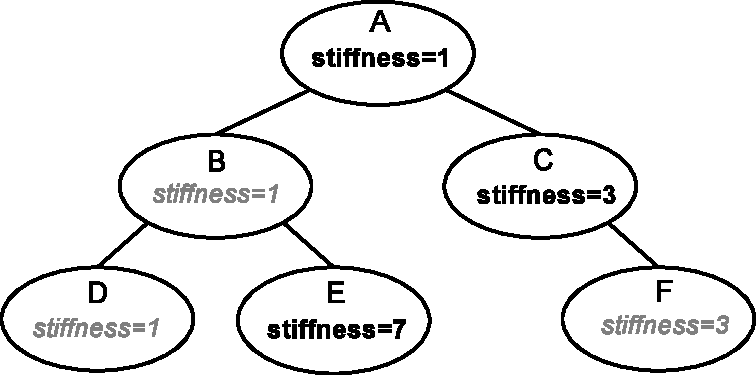
\includegraphics[width=3.75in]{images/inheritedProperties}
\end{center}
\caption{Inheritance of a property named {\it stiffness} among
a component hierarchy. Explicit settings are in bold; inherited settings
are in gray italic.}
\label{inheritedProperties:fig}
\end{figure}

Composite properties are possible, in which a property value is a
composite object that in turn has sub-properties. A good example of
this is the {\tt RenderProps} class, which is
associated with the property {\tt renderProps} for renderable objects
and which itself can have a number of sub-properties such as {\tt
visible}, {\tt faceStyle}, {\tt faceColor}, {\tt lineStyle}, {\tt
lineColor}, etc.

Properties can be declared to be {\tt inheritable}, so that their
values can be inherited from the same properties hosted by ancestor
components further up the component hierarchy. Inheritable properties
require a more elaborate declaration and are associated with a {\it
mode} which may be either {\tt Explicit} or {\tt Inherited}.  If a
property's mode is inherited, then its value is obtained from
the closest ancestor exposing the same property whose mode is
explicit. In Figure (\ref{inheritedProperties:fig}), the property {\it
stiffness} is explicitly set in components A, C, and E, and inherited
in B and D (which inherit from A) and F (which inherits from C).

\section{Creating an application model}
\label{CreatingAnApplication:sec}

ArtiSynth applications are created by writing and compiling
an {\it application model} that is a subclass of {\tt RootModel}.
This application-specific root model is then loaded and run by the
ArtiSynth program.

The code for the application model should:

\begin{itemize}

\item Declare a no-args constructor

\item Override the {\tt RootModel}
\javamethod*[artisynth.core.workspace.RootModel]{build()}
method to construct the application.

\end{itemize}

ArtiSynth can load a model either using the build method
or by reading it from a file:

\begin{description}

\item[Build method] \mbox{}

ArtiSynth creates an instance of the
model using the no-args constructor, assigns it a name
(which is either user-specified or the simple name of the class), and
then calls the {\tt build()} method to perform the actual
construction.

\item[Reading from a file] \mbox{}

ArtiSynth creates an instance of the
model using the no-args constructor, and then the model is named
and constructed by reading the file.

\end{description}

The no-args constructor should perform whatever initialization is
required in both cases, while the {\tt build()} method takes the place of the
file specification. Unless a model is originally created using a file
specification (which is very tedious), the first time
creation of a model will almost always entail using the {\tt build()}
method.

The general template for application model code looks like this:

\begin{lstlisting}[]
package artisynth.models.experimental; // package where the model resides
import artisynth.core.workspace.RootModel;
... other imports ...

public class MyModel extends RootModel {

   // no-args constructor
   public MyModel() {
      ... basic initialization ...
   }

   // build method to do model construction
   public void build (String[] args) {
      ... code to build the model ....
   }
}
\end{lstlisting}
Here, the model itself is called {\tt MyModel}, and is defined in the
(hypothetical) 
package {\tt artisynth.models.experimental} (placing models in the super
package {\tt artisynth.models} is common practice but not
necessary).

\begin{sideblock}
Note: The {\tt build()} method was only introduced in ArtiSynth
3.1. Prior to that, application models were constructed using a
constructor taking a {\tt String} argument supplying the name of the
model. This method of model construction still works but is
deprecated.
\end{sideblock}

\subsection{Implementing the build() method}

As mentioned above, the {\tt build()} method is responsible for actual
model construction.  Many applications are built using a single
top-level {\tt MechModel}.  Build methods for these may look
like the following:
\begin{lstlisting}[]
   public void build (String[] args) {
      MechModel mech = new MechModel("mech");
      addModel (mech);

      ... create and add components to the mech model ...
      ... create and add any needed agents to the root model ...

   }
\end{lstlisting}
First, a \javaclass[artisynth.core.mechmodels]{MechModel} is created
(with the name {\tt "mech"} in this example, although any name, or no
name, may be given) and added to the list of models in the root
model. Subsequent code then creates and adds the components required
by the {\tt MechModel}, as described in Sections
\ref{MechModelsI:sec}, \ref{MechModelsII:sec} and \ref{FEMModels:sec}.
The {\tt build()} method also creates and adds to the root model any
agents required by the application (controllers, probes, etc.), as
described in Section \ref{SimulationControl:sec}.

When constructing a model, there is no fixed order in which components
need to be added. For instance, in the above example, {\tt
addModel(mech)} could be called near the end of the {\tt build()}
method rather than at the beginning. The only restriction is that when
a component is added to the hierarchy, all other components that it
refers to should already have been added to the hierarchy. For
instance, an axial spring (Section \ref{ParticlesAndSprings:sec})
refers to two points. When it is added to the hierarchy, those two
points should already be present in the hierarchy.

The {\tt build()} method supplies a {\tt String} array as an argument.
(This is analogous to the {\tt args} argument passed to static {\tt
main()} methods.) These is reserved for future use to supply
application-supplied arguments.

\subsection{Making models visible to ArtiSynth}

In order to load an application model into ArtiSynth, the classes
associated with its implementation must be made visible to ArtiSynth.
This usually involves adding the top-level class directory associated
with the application code to the classpath used by ArtiSynth.

\begin{sideblock}
The demonstration models referred to in this guide belong to the
package {\tt artisynth.demos.tutorial} and are already visible to
ArtiSynth.
\end{sideblock}

In most current ArtiSynth projects, classes are stored in
a directory tree separate from the source code, with the top-level
class directory named {\tt classes}, located one level below
the project root directory. A typical top-level class directory
might be stored in a location like this:
\begin{verbatim}
  /home/joeuser/artisynthProjects/classes
\end{verbatim}
In the example shown in Section \ref{CreatingAnApplication:sec}, the
model was created in the package {\tt artisynth.models.experimental}.
Since Java classes are arranged in a directory structure that mirrors
package names, with respect to the sample project directory shown
above, the model class would be located in
\begin{verbatim}
  /home/joeuser/artisynthProjects/classes/artisynth/models/experimental
\end{verbatim}

At present there are three ways to make top-level class directories
known to ArtiSynth:

\begin{description}

\item[Add projects to your Eclipse launch configuration]\mbox{}

If you are using the Eclipse IDE, then you can add the project in
which are developing your model code to the launch configuration that
you use to run ArtiSynth. Other IDEs will presumably provide similar
functionality.

\item[Add the directories to the EXTCLASSPATH file]\mbox{}

You can explicitly list class directories in the file EXTCLASSPATH,
located in the ArtiSynth root directory (it may be necessary to create
this file).

\item[Add the directories to your CLASSPATH environment variable]\mbox{}

If you are running ArtiSynth from the command line, using the {\tt
artisynth} command (or {\tt artisynth.bat} on Windows), then you can
define a CLASSPATH environment variable in your environment and add
the needed directories to this.

\end{description}

All of these methods are described in more detail in the ``Installing
External Models and Packages'' section of the ArtiSynth Installation
Guide (available for \href{../installation/linuxInstallation.html}{Linux}, 
\href{../installation/windowsInstallation.html}{Windows}, and
\href{../installation/macosInstallation.html}{MacOS}).

\subsection{Loading and running a model}
\label{LoadingAndRunning:sec}

If a model's classes are visible to ArtiSynth, then it may be loaded
into ArtiSynth in several ways:

\begin{description}

\item[Loading by class path]\mbox{}

A model may be loaded by directly by choosing {\sf File > Load from
class ...} and directly specifying its class name. It is also possible
to use the {\tt -model <classname>} command line argument to have a
model loaded directly into ArtiSynth when it starts up.

\item[Loading from the Models menu]\mbox{}

A faster way to load a model is by selecting it in one of the {\sf
Models} submenus. This may require editing the model menu
configuration files.

\item[Loading from a file]\mbox{}

If a model has previously been saved to a file, it may be loaded from
that file by choosing {\sf File > Load model ...}.

\end{description}

These methods are described in detail in the 
section ``Loading and Simulating Models'' of the
\href{../uiguide/uiguide.html}{
ArtiSynth User Interface Guide}.

\begin{sideblock}
The demonstration models referred to in this guide should already
be present in the models menu and may be loaded
from the submenu {\sf Models > All demos > tutorial}.
\end{sideblock}

Once a model is loaded, it can be simulated, or {\it run}.
Simulation
of the model can then be started, paused, single-stepped, or reset
using the play controls (Figure \ref{PlayControlsFig})
located at the upper right of the ArtiSynth window frame.

\begin{figure}[ht]
\begin{center}
\iflatexml
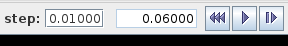
\includegraphics[]{../installation/images/playControls}
\else
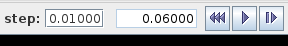
\includegraphics[width=2.5in]{../installation/images/playControls}
\fi
\end{center}
\caption{The ArtiSynth play controls. From left to right: step size
control, current simulation time, and the reset, play/pause, and
single-step buttons.}%
\label{PlayControlsFig}
\end{figure}

Comprehensive information on exploring and interacting with models is
given in the
\href{../uiguide/uiguide.html}
{ArtiSynth User Interface Guide}.



\section{Supporting classes}

ArtiSynth uses a large number of supporting classes, mostly defined in
the super package {\tt maspack}, for handling mathematical and
geometric quantities. Those that are refered to in this manual are
summarized in this section.

\subsection{Vectors and matrices}

Among the most basic classes are those used to implement vectors and
matrices, defined in {\tt mapack.matrix}. All vector classes implement
the interface \javaclass[maspack.matrix]{Vector} and all matrix
classes implement \javaclass[maspack.matrix]{Matrix}, which provide a
number of standard methods for setting and accessing values and
reading and writing from I/O streams. 

General sized vectors and matrices are implemented by
\javaclass[maspack.matrix]{VectorNd} and
\javaclass[maspack.matrix]{MatrixNd}. These provide all the usual
methods for linear algebra operations such as addition, scaling, and
multiplication:
%
\begin{lstlisting}[]
  VectorNd v1 = new VectorNd (5);        // create a 5 element vector
  VectorNd v2 = new VectorNd (5); 
  VectorNd vr = new VectorNd (5); 
  MatrixNd M = new MatrixNd (5, 5);      // create a 5 x 5 matrix

  M.setIdentity();                       // M = I
  M.scale (4);                           // M = 4*M

  v1.set (new double[] {1, 2, 3, 4, 5}); // set values
  v2.set (new double[] {0, 1, 0, 2, 0});
  v1.add (v2);                           // v1 += v2
  M.mul (vr, v1);                        // vr = M*v1

  System.out.println ("result=" + vr.toString ("%8.3f"));
\end{lstlisting}
%
As illustrated in the above example, vectors and matrices both provide
a {\tt toString()} method that allows their elements to be formated
using a C-printf style format string. This is useful for providing
concise and uniformly formatted output, particularly for diagnostics.
The output from the above example is
%
\begin{verbatim}
  result=   4.000   12.000   12.000   24.000   20.000
\end{verbatim}
%
Detailed specifications for the format string are provided in the
documentation for \javamethod[maspack.util]{NumberFormat.set(String)}.
If either no format string, or the string {\tt "\%g"}, is specified,
{\tt toString()} formats all numbers using the full-precision output
provided by {\tt Double.toString(value)}.

For computational efficiency, a number of fixed-size vectors and
matrices are also provided. The most commonly used are those defined
for three dimensions, including \javaclass[maspack.matrix]{Vector3d}
and \javaclass[maspack.matrix]{Matrix3d}:
%
\begin{lstlisting}[]
  Vector3d v1 = new Vector3d (1, 2, 3);
  Vector3d v2 = new Vector3d (3, 4, 5);
  Vector3d vr = new Vector3d ();
  Matrix3d M = new Matrix3d();

  M.set (1, 2, 3,  4, 5, 6,  7, 8, 9);

  M.mul (vr, v1);        // vr = M * v1
  vr.scaledAdd (2, v2);  // vr += 2*v2;
  vr.normalize();        // normalize vr
  System.out.println ("result=" + vr.toString ("%8.3f"));
\end{lstlisting}
%

\subsection{Rotations and transformations}
\label{RigidTransform3d:sec}

{\tt maspack.matrix} contains a number classes that implement rotation
matrices, rigid transforms, and affine transforms. 

Rotations (Section \ref{Rotations:sec}) are commonly described using a
\javaclass[maspack.matrix]{RotationMatrix3d}, which implements a
rotation matrix and contains numerous methods for setting rotation
values and transforming other quantities. Some of the more commonly
used methods are:
%
\begin{lstlisting}[]
   RotationMatrix3d();         // create and set to the identity
   RotationMatrix3d(u, angle); // create and set using an axis-angle

   setAxisAngle (u, ang);      // set using an axis-angle
   setRpy (roll, pitch, yaw);  // set using roll-pitch-yaw angles
   setEuler (phi, theta, psi); // set using Euler angles
   invert ();                  // invert this rotation
   mul (R)                     // post multiply this rotation by R
   mul (R1, R2);               // set this rotation to R1*R2
   mul (vr, v1);               // vr = R*v1, where R is this rotation
\end{lstlisting}
%
Rotations can also be described by
\javaclass[maspack.matrix]{AxisAngle}, which characterizes a rotation
as a single rotation about a specific axis.

Rigid transforms (Section \ref{RigidTransforms:sec}) are used by
ArtiSynth to describe a rigid body's pose, as well as its relative
position and orientation with respect to other bodies and coordinate
frames.  They are implemented by
\javaclass[maspack.matrix]{RigidTransform3d}, which exposes its
rotational and translational components directly through the fields
{\tt R} (a {\tt RotationMatrix3d}) and {\tt p} (a {\tt
Vector3d}). Rotational and translational values can be set and
accessed directly through these fields.  In addition, {\tt
RigidTransform3d} provides numerous methods, some of the more commonly
used of which include:
%
\begin{lstlisting}[]
   RigidTransform3d();         // create and set to the identity
   RigidTransfrom3d(x, y, z);  // create and set translation to x, y, z

   // create and set translation to x, y, z and rotation to roll-pitch-yaw
   RigidTransfrom3d(x, y, z, roll, pitch, yaw);

   invert ();                  // invert this transform
   mul (T)                     // post multiply this transform by T
   mul (T1, T2);               // set this transform to T1*T2
   mulLeftInverse (T1, T2);    // set this transform to inv(T1)*T2
\end{lstlisting}
%

Affine transforms (Section \ref{AffineTransforms:sec}) are used by
ArtiSynth to effect scaling and shearing transformations on
components. They are implemented by
\javaclass[maspack.matrix]{AffineTransform3d}.

Rigid transformations are actually a specialized form of affine
transformation in which the basic transform matrix equals a rotation.
{\tt RigidTransform3d} and {\tt AffineTransform3d} hence both derive
from the same base class
\javaclass[maspack.matrix]{AffineTransform3dBase}.

\subsection{Points and Vectors}

The rotations and transforms described above can be used to transform
both vectors and points in space.

Vectors are most commonly implemented using
\javaclass[maspack.matrix]{Vector3d}, while points can be implemented
using the subclass \javaclass[maspack.matrix]{Point3d}.  The only
difference between {\tt Vector3d} and {\tt Point3d} is that the former
ignores the translational component of rigid and affine transforms;
i.e., as described in Sections \ref{RigidTransforms:sec} and
\ref{AffineTransforms:sec}, a vector {\tt v} has
an implied homogeneous representation of
%
\begin{equation}
\v^* \equiv \matl \v \\ 0 \matr,
\end{equation}
%
while the representation for a point {\tt p} is
%
\begin{equation}
\p^* \equiv \matl \p \\ 1 \matr.
\end{equation}
%

Both classes provide a number of methods for applying rotational and
affine transforms. Those used for rotations are
%
\begin{lstlisting}
  void transform (R);             // this = R * this
  void transform (R, v1);         // this = R * v1
  void inverseTransform (R);      // this = inverse(R) * this
  void inverseTransform (R, v1);  // this = inverse(R) * v1
\end{lstlisting}
%
where {\tt R} is a rotation matrix and {\tt v1} is a vector (or a point
in the case of {\tt Point3d}).

The methods for applying rigid or affine transforms include:
\begin{lstlisting}
  void transform (X);             // transforms this by X         
  void transform (X, v1);         // sets this to v1 transformed by X
  void inverseTransform (X);      // transforms this by the inverse of X
  void inverseTransform (X, v1);  // sets this to v1 transformed by inverse of X
\end{lstlisting}
where {\tt X} is a rigid or affine transform.
As described above, in the case of {\tt Vector3d}, these methods
ignore the translational part of the transform and apply only the
matrix component ({\tt R} for a {\tt RigidTransform3d} and {\tt A} for
an {\tt AffineTransform3d}).
In particular, that means that for a {\tt RigidTransform3d} given by {\tt X}
and a {\tt Vector3d} given by {\tt v},
the method calls
%
\begin{lstlisting}
  v.transform (X.R)
  v.transform (X)
\end{lstlisting}
%
produce the same result.

\subsection{Spatial vectors and inertias}
\label{SpatialVectors:sec}

The velocities, forces and inertias associated with 3D coordinate
frames and rigid bodies are represented using the 6 DOF spatial
quantities described in Sections \ref{SpatialVelocitiesAndForces:sec}
and \ref{SpatialInertia:sec}. These are implemented by classes in the
package {\tt maspack.spatialmotion}.

Spatial velocities (or twists) are implemented by
\javaclass[maspack.spatialmotion]{Twist}, which exposes its
translational and angular velocity components through the publicly
accessible fields {\tt v} and {\tt w}, while spatial forces (or
wrenches) are implemented by
\javaclass[maspack.spatialmotion]{Wrench}, which exposes its
translational force and moment components through the publicly
accessible fields {\tt f} and {\tt m}.

Both {\tt Twist} and {\tt Wrench} contain methods for algebraic
operations such as addition and scaling. They also contain {\tt
transform()} methods for applying rotational and rigid transforms.
The rotation methods simply transform each component by the supplied
rotation matrix. The rigid transform methods, on the other hand,
assume that the supplied argument represents a transform between two
frames fixed within a rigid body, and transform the twist or wrench
accordingly, using either (\ref{XvelAB:eqn}) or (\ref{XforceAB:eqn}).

The spatial inertia for a rigid body is implemented by
\javaclass[maspack.spatialmotion]{SpatialInertia}, which contains a
number of methods for setting its value given various mass, center of
mass, and inertia values, and querying the values of its components.
It also contains methods for scaling and adding, transforming between
coordinate systems, inversion, and multiplying by spatial vectors.

\subsection{Meshes}
\label{Meshes:sec}

ArtiSynth makes extensive use of 3D meshes, which are defined in {\tt
maspack.geometry}.  They are used for a variety of purposes, including
visualization, collision detection, and computing physical properties
(such as inertia or stiffness variation within a finite element
model).

A mesh is essentially a collection of vertices
(i.e., points) that are topologically connected in some way.  All
meshes extend the abstract base class
\javaclass[maspack.geometry]{MeshBase}, which supports the vertex
definitions, while subclasses provide the topology.

Through {\tt MeshBase}, all meshes provide methods for
adding and accessing vertices. Some of these include:
%
\begin{lstlisting}[]
  int getNumVertices();              // return the number of vertices
  Vertex3d getVertex (int idx);      // return the idx-th vertex
  void addVertex (Vertex3d vtx);     // add vertex vtx to the mesh
  Vertex3d addVertex (Point3d p);    // create and return a vertex at position p
  void removeVertex (Vertex3d vtx);  // remove vertex vtx for the mesh
  ArrayList<Vertex3d> getVertices(); // return the list of vertices
\end{lstlisting}
%
Vertices are implemented by \javaclass[maspack.geometry]{Vertex3d},
which defines the position of the vertex (returned by the method
\javamethod*[maspack.geometry.Vertex3d]{getPosition()}), and also
contains support for topological connections. In addition, each vertex
maintains an index, obtainable via
\javamethod*[maspack.geometry.Vertex3d]{getIndex()}, that equals the
index of its location within the mesh's vertex list. This makes it
easy to set up parallel array structures for augmenting mesh vertex
properties.

Mesh subclasses currently include:

\begin{description}

\item[\protect{\javaclass[maspack.geometry]{PolygonalMesh}}]\mbox{}

Implements a 2D surface
mesh containing faces implemented using half-edges.

\item[\protect{\javaclass[maspack.geometry]{PolylineMesh}}]\mbox{}

Implements a mesh
consisting of connected line-segments (polylines).

\item[\protect{\javaclass[maspack.geometry]{PointMesh}}]\mbox{}

Implements a point cloud with
no topological connectivity.

\end{description}

\javaclass[maspack.geometry]{PolygonalMesh} is used quite extensively
and provides a number of methods for implementing faces, including:
%
\begin{lstlisting}[]
  int getNumFaces();              // return the number of faces
  Face getFace (int idx);         // return the idx-th face
  Face addFace (int[] vidxs);     // create and add a face from specified vertex indices
  void removeFace (Face f);       // remove the face f
  ArrayList<Face> getFaces();     // return the list of faces
\end{lstlisting}
%
The class \javaclass[maspack.geometry]{Face} implements a face as a
counter-clockwise arrangement of vertices linked together by
half-edges (class \javaclass[maspack.geometry]{HalfEdge}).
{\tt Face} also supplies a face's (outward facing) normal
via 
\javamethod[maspack.geometry.Face]{getNormal()}.

Some mesh uses within ArtiSynth, such as collision detection, require a
{\it triangular} mesh; i.e., one where all faces have three vertices.
The method \javamethod[maspack.geometry.PolygonalMesh]{isTriangular()}
can be used to check for this. Meshes that are not triangular can be
made triangular using 
\javamethod[maspack.geometry.PolygonalMesh]{triangulate()}.

\subsubsection{Mesh creation}

It is possible to create a mesh by direct construction. For example,
the following code fragment creates a simple closed tetrahedral
surface:
%
\begin{lstlisting}[]
   // a simple four-faced tetrahedral mesh 
   PolygonalMesh mesh = new PolygonalMesh();
   mesh.addVertex (0, 0, 0);
   mesh.addVertex (1, 0, 0);
   mesh.addVertex (0, 1, 0);
   mesh.addVertex (0, 0, 1);
   mesh.addFace (new int[] { 0, 2, 1 });
   mesh.addFace (new int[] { 0, 3, 2 });
   mesh.addFace (new int[] { 0, 1, 3 });
   mesh.addFace (new int[] { 1, 2, 3 });      
\end{lstlisting}
%

However, meshes are more commonly created using either one of the
factory methods supplied by \javaclass[maspack.geometry]{MeshFactory},
or by reading a definition from a file (Section \ref{MeshFileIO:sec}).

Some of the more commonly used factory methods for creating polyhedral
meshes include:
%
\begin{lstlisting}[]
  MeshFactory.createSphere (radius, nslices, nlevels);
  MeshFactory.createBox (widthx, widthy, widthz);
  MeshFactory.createCylinder (radius, height, nslices);
  MeshFactory.createPrism (double[] xycoords, height);
  MeshFactory.createTorus (rmajor, rminor, nmajor, nminor);
\end{lstlisting}
%
Each factory method creates a mesh in some standard coordinate
frame. After creation, the mesh can be transformed using the
\javamethodAlt{maspack.geometry.MeshBase.transform(AffineTransform3dBase)}%
{transform(X)} method, where {\tt X} is either a rigid transform (
\javaclass[maspack.matrix]{RigidTransform3d}) or a more general affine
transform (\javaclass[maspack.matrix]{AffineTransform3d}).
For example, to create a rotated box centered on $(5, 6, 7)$,
one could do:
%
\begin{lstlisting}[]
  // create a box centered at the origin with widths 10, 20, 30:
  PolygonalMesh box = MeshFactor.createBox (10, 20, 20);

  // move the origin to 5, 6, 7 and rotate using roll-pitch-yaw
  // angles 0, 0, 45 degrees:
  box.transform (
     new RigidTransform3d (5, 6, 7,  0, 0, Math.toRadians(45)));
\end{lstlisting}
%
One can also scale a mesh using
\javamethodAlt{maspack.geometry.MeshBase.scale(double)}{scale(s)},
where {\tt s} is a single scale factor, or
\javamethodAlt{maspack.geometry.MeshBase.scale(double,double,double)}%
{scale(sx,sy,sz)}, where {\tt sx}, {\tt sy}, and {\tt sz} are separate
scale factors for the x, y and z axes. This provides a useful way to
create an ellipsoid:
%
\begin{lstlisting}[]
   // start with a unit sphere with 12 slices and 6 levels ...
  PolygonalMesh ellipsoid = MeshFactor.createSphere (1.0, 12, 6);

  // and then turn it into an ellipsoid by scaling about the axes:
  ellipsoid.scale (1.0, 2.0, 3.0);
\end{lstlisting}
%
\javaclass[maspack.geometry]{MeshFactory} can also be used to create
new meshes by performing boolean operations on existing ones:
%
\begin{lstlisting}[]
  MeshFactory.getIntersection (mesh1, mesh2);
  MeshFactory.getUnion (mesh1, mesh2);
  MeshFactory.getSubtraction (mesh1, mesh2);
\end{lstlisting}
%

\subsubsection{Reading and writing mesh files}
\label{MeshFileIO:sec}

The package {\tt maspack.geometry.io} supplies a number of classes for
writing and reading meshes to and from files of different formats.

Some of the supported formats and their associated readers and writers
include:

\begin{tabular}{|lll|}
\hline
Extension & Format & Reader/writer classes \\
\hline
.obj & Alias Wavefront & \tt WavefrontReader, WavefrontWriter \\
.ply & Polygon file format & \tt PlyReader, PlyWriter \\
.stl & STereoLithography & \tt StlReader, StlWriter \\
.gts & GNU triangulated surface & \tt GtsReader, GtsWriter \\
.off & Object file format & \tt OffReader, OffWriter \\
\hline
\end{tabular}

The general usage pattern for these classes is to construct the
desired reader or writer with a path to the desired file, and then
call {\tt readMesh()} or {\tt writeMesh()} as appropriate:
%
\begin{lstlisting}[]
   // read a mesh from a .obj file:
   WavefrontReader reader = new WavefrontReader ("meshes/torus.obj");
   PolygonalMesh mesh = null;
   try {
      mesh = reader.readMesh();
   }
   catch (IOException e) {
      System.err.println ("Can't read mesh:");
      e.printStackTrace();
   }
\end{lstlisting}
%
Both {\tt readMesh()} and {\tt writeMesh()} may throw I/O exceptions,
which must be either caught, as in the example above, or
thrown out of the calling routine.

For convenience, one can also use the classes
\javaclass[maspack.geometry.io]{GenericMeshReader} or
\javaclass[maspack.geometry.io]{GenericMeshWriter}, which internally
create an appropriate reader or writer based on the file
extension. This enables the writing of code
that does not depend on the file format:
%
\begin{lstlisting}[]
   String fileName;
   ...
   PolygonalMesh mesh = null;
   try {
      mesh = (PolygonalMesh)GenericMeshReader.readMesh(fileName);
   }
   catch (IOException e) {
      System.err.println ("Can't read mesh:");
      e.printStackTrace();
   }
\end{lstlisting}
%
Here, {\tt fileName} can refer to a mesh of any format supported by
{\tt GenericMeshReader}. Note that the mesh returned by {\tt
readMesh()} is explicitly cast to {\tt PolygonalMesh}.  This is
because {\tt readMesh()} returns the superclass {\tt MeshBase}, since
the default mesh created for some file formats may be different from
{\tt PolygonalMesh}.


%!TEX root = modelguide.tex

\section{Mechanical Models I}
\label{MechModelsI:sec}

This section details how to build basic multibody-type mechanical
models consisting of particles, springs, rigid bodies, joints, and
other constraints.

\subsection{Springs and particles}
\label{ParticlesAndSprings:sec}

The most basic type of mechanical model consists simply of particles
connected together by axial springs.  Particles are implemented by the
class \javaclass[artisynth.core.mechmodels]{Particle}, which is a
dynamic component containing a three-dimensional position state, a
corresponding velocity state, and a mass. It is an instance of the
more general base class \javaclass[artisynth.core.mechmodels]{Point},
which is used to also implement spatial points such as {\tt markers}
which do not have a mass.

\subsubsection{Axial springs and materials}
\label{AxialSprings:sec}

An axial spring is a simple spring that connects two points and is
implemented by the class
\javaclass[artisynth.core.mechmodels]{AxialSpring}. This is a {\it
force effector} component that exerts equal and opposite forces on the
two points, along the line separating them, with a magnitude $f$ that
is a function $f(l, \dot l)$ of the distance $l$ between the points,
and the distance derivative $\dot l$.

Each axial spring is associated with an {\it axial material},
implemented by a subclass of
\javaclass[artisynth.core.materials]{AxialMaterial}, that specifies
the function $f(l, \dot l)$. The most basic type of axial material is
a \javaclass[artisynth.core.materials]{LinearAxialMaterial}, which
determines $f$ according to the linear relationship
%
\begin{equation}
f(l, \dot l) = k (l-l_0) + d \dot l
\end{equation}
%
where $l_0$ is the rest length and $k$ and $d$ are the stiffness and
damping terms. Both $k$ and $d$ are properties of the material, while
$l_0$ is a property of the spring.

Axial springs are assigned a linear axial material by default.  More
complex, non-linear axial materials may be defined in the package {\tt
artisynth.core.materials}. Setting or querying a spring's material
may be done with the methods {\tt setMaterial()} and {\tt
getMaterial()}.

\subsubsection{Example: A simple particle-spring model}
\label{ParticleSpringExample:sec}

\begin{figure}[t]
\begin{center}
\iflatexml
 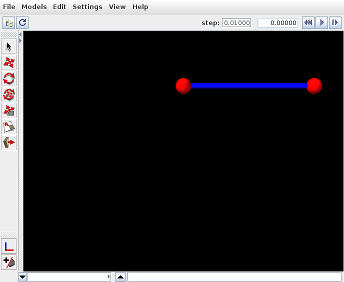
\includegraphics[]{images/ParticleSpring}
\else
 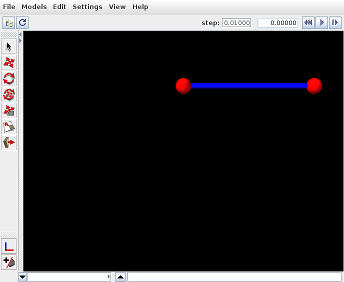
\includegraphics[width=3.75in]{images/ParticleSpring}
\fi
\end{center}
\caption{ParticleSpring model loaded into ArtiSynth.}
\label{ParticleSpring:fig}
\end{figure}

An complete application model that implements a simple particle-spring
model is given below. 
\lstset{numbers=left}
\lstinputlisting{../../src/artisynth/demos/tutorial/ParticleSpring.java}
\lstset{numbers=none}

Line 1 of the source defines the package in which the model class will
reside, in this case {\tt artisynth.demos.tutorial}. Lines 3-8 import
definitions for other classes that will be used.

The model application class is named {\tt ParticleSpring} and declared
to extend {\tt RootModel} (line 13), and the {\tt build()} method
definition begins at line 15. (A no-args constructor is also needed,
but because no other constructors are defined, the compiler creates
one automatically.)

To begin, the {\tt build()} method creates a {\tt MechModel} named
{\tt "mech"}, and then adds it to the {\tt models} list of the root model
using the {\tt addModel()} method (lines 18-19). Next, two particles,
{\tt p1} and {\tt p2}, are created, with masses equal to 2 and initial
positions at 0, 0, 0, and 1, 0, 0, respectively (lines 22-23). Then an
axial spring is created, with end points set to {\tt p1} and {\tt p2},
and assigned a linear material with a stiffness and damping of 20 and
10 (lines 24-27). Finally, after the particles and the spring are
created, they are added to the {\tt particles} and {\tt axialSprings}
lists of the {\tt MechModel} using the methods {\tt
addParticle()} and {\tt addAxialSpring()} (lines 30-32).

At this point in the code, both particles are defined to be
dynamically controlled, so that running the simulation would cause
both to fall under the {\tt MechModel}'s default gravity acceleration
of $(0, 0, -9.8)$. However, for this example, we want the first
particle to remain fixed in place, so we set it to be {\it
non-dynamic} (line 34), meaning that the physical simulation will not
update its position in response to forces (Section
\ref{DynamicVsParametric:sec}).

The remaining calls control aspects of how the model is graphically
rendered.  {\tt setBounds()} (line 37) increases the model's
``bounding box'' so that by default it will occupy a larger part of
the viewer frustum. The covenience method {\tt
RenderProps.setSphericalPoints()} is used to set points {\tt p1} and
{\tt p2} to render as solid red spheres with a radius of 0.06, while
{\tt RenderProps.setCylindricalLines()} is used to set {\tt spring} to
render as a solid blue cylinder with a radius of 0.02. More details
about setting render properties are given in Section
\ref{RenderProperties:sec}.

To run this example in ArtiSynth, select {\sf All demos > tutorial >
ParticleSpring} from the {\sf Models} menu. The model should load and
initially appear as in Figure \ref{ParticleSpring:fig}.  Running
the model (Section \ref{LoadingAndRunning:sec}) will
cause the second particle to fall and swing about under gravity.

\subsubsection{Dynamic, parametric, and attached components}
\label{DynamicVsParametric:sec}

By default, a dynamic component is advanced through time in response
to the forces applied to it. However, it is also possible to set a
dynamic component's {\tt dynamic} property to {\tt false}, so that it
does not respond to force inputs.  As shown in the example above, this
can be done using the method
{\tt setDynamic()}:
%
\begin{verbatim}
  comp.setDynamic (false);
\end{verbatim}
%
The method
\javamethod*[artisynth.core.mechmodels.DynamicComponent]{isDynamic()}
can be used to query the {\tt dynamic} property.

Dynamic components can also be {\it attached} to other dynamic
components (as mentioned in Section \ref{PhysicsSimulation:sec}) so
that their positions and velocities are controlled by the {\it master}
components that they are attached to.  To attach a dynamic component,
one creates an {\tt AttachmentComponent} specifying the attachment
connection and adds it to the {\tt MechModel}, as described in Section
\ref{Attachments:sec}.  The method
\javamethod*[artisynth.core.mechmodels.DynamicComponent]{isAttached()}
can be used to determine if a component is attached, and if it is,
\javamethod*[artisynth.core.mechmodels.DynamicComponent]{getAttachment()}
can be used to find the corresponding {\tt AttachmentComponent}.

Overall, a dynamic component can be in one of three states:

\begin{description}

\item[active]\mbox{}

Component is dynamic and unattached. The method
\javamethod*[artisynth.core.mechmodels.DynamicComponent]{isActive()}
returns {\tt true}. The component will move in response to forces.

\item[parametric]\mbox{}

Component is not dynamic, and is unattached. 
The method
\javamethod*[artisynth.core.mechmodels.DynamicComponent]{isParametric()}
returns {\tt true}.
The component will either remain
fixed, or will move around in response to external inputs specifying
the component's position and/or velocity. One way to supply such
inputs is to use controllers or input probes, as described in
Section \ref{SimulationControl:sec}.

\item[attached]\mbox{}

Component is attached. The method
\javamethod*[artisynth.core.mechmodels.DynamicComponent]{isAttached()}
returns {\tt true}. The component will move so as to follow the other
master component(s) to which it is attached.

\end{description}

\subsubsection{Custom axial materials}

Application authors may create their
own axial materials by subclassing 
\javaclass[artisynth.core.materials]{AxialMaterial}
and overriding the functions
%
\begin{lstlisting}[]
  double computeF (l, ldot, l0, excitation);
  double computeDFdl (l, ldot, l0, excitation);
  double computeDFdldot (l, ldot, l0, excitation);
  boolean isDFdldotZero ();
\end{lstlisting}
%
where {\tt excitation} is an additional {\it excitation} signal $a$, which
is used to implement active springs and which in particular is used to
implement axial muscles (Section \ref{PointToPointMuscles:sec}), for
which $a$ is usually in the range $[0, 1]$.

The first three methods should return the values of 
%
\begin{equation}
f (l, \dot l, a), \quad
\frac{\partial f(l, \dot l, a)}{\partial l}, \quad \text{and} \quad
\frac{\partial f(l, \dot l, a)}{\partial \dot l},
\end{equation}
%
respectively, while the last method should return {\tt true} if
$\partial f(l, \dot l, a) / \partial \dot l \equiv 0$; i.e., if it is
always equals to 0.

\subsubsection{Damping parameters}

Mechanical models usually contain damping forces in addition to
spring-type restorative forces. Damping generates forces that reduce
dynamic component velocities, and is usually the major source of
energy dissipation in the model. Damping forces can be generated by
the spring components themselves, as described above.

A general damping can be set for all particles by setting the
{\tt MechModel}'s {\tt pointDamping} property. This causes
a force
%
\begin{equation}
\f_i = -d_p \v_i \label{eqn:pointdamping}
\end{equation}
%
to be applied to all particles, where $d_p$ is the value of the {\tt
pointDamping} and $\v_i$ is the particle's velocity.

{\tt pointDamping} can be set and queried using the {\tt MechModel}
methods
%
\begin{lstlisting}[]
  setPointDamping (double d);
  double getPointDamping();
\end{lstlisting}
%

\begin{sideblock}
In general, whenever a component has a property {\tt propX}, that
property can be set and queried in code using methods of the form
\begin{verbatim}
  setPropX (T d);
  T getPropX();
\end{verbatim}
where {\tt T} is the type associated with the property.
\end{sideblock}

{\tt pointDamping} can also be set for particles individually.  This
property is {\it inherited} (Section
\ref{CompositeInheritableProperties:sec}), so that if not set
explicitly, it inherits the nearest explicitly set value in an
ancestor component.

\subsection{Rigid bodies}

Rigid bodies are implemented in ArtiSynth by the class
\javaclass[artisynth.core.mechmodels]{RigidBody}, which is a dynamic
component containing a six-dimensional position and orientation state,
a corresponding velocity state, an inertia, and an optional surface
mesh.

A rigid body is associated with its own 3D spatial coordinate frame,
and is a subclass of the more general
\javaclass[artisynth.core.mechmodels]{Frame} component.
The combined position and orientation of this frame with respect to
world coordinates defines the body's {\it pose}, and the associated 6
degrees of freedom describe its ``position'' state.

\subsubsection{Frame markers}
\label{FrameMarkers:sec}

\begin{figure}[t]
\begin{center}
 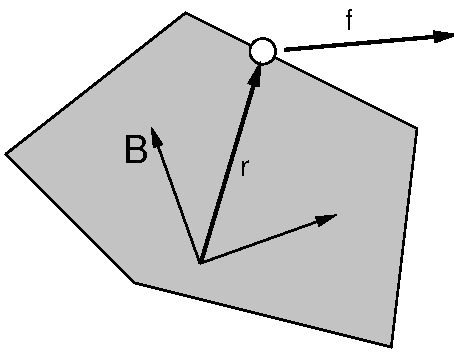
\includegraphics[width=2.5in]{images/frameMarker}
\end{center}
\caption{A force $\f$ applied to a frame marker attached to a rigid
body. The marker is located at the point $\r$ with respect to the body
coordinate frame B.}
\label{frameMarker:fig}
\end{figure}

ArtiSynth makes extensive use of {\it markers}, which are (massless)
points attached to dynamic components in the model. Markers are used
for graphical display, implementing attachments, and transmitting
forces back onto the underlying dynamic components.

A {\it frame marker} is a marker that can be attached to a
\javaclass[artisynth.core.mechmodels]{Frame}, and most commonly to a
\javaclass[artisynth.core.mechmodels]{RigidBody} (Figure
\ref{frameMarker:fig}). They are frequently used to provide the
anchor points for attaching springs and, more generally, applying
forces to the body.

Frame markers are implemented by the class
\javaclass[artisynth.core.mechmodels]{FrameMarker}, which
is a subclass of
\javaclass[artisynth.core.mechmodels]{Point}.
The methods
%
\begin{lstlisting}[]
  Point3d getLocation();
  void setLocation (Point3d r);
\end{lstlisting}
%
get and set the marker's location $\r$ with respect to the frame's
coordinate system. When a 3D force $\f$ is applied to the marker, it
generates a spatial force $\hat\f$ (Section
\ref{SpatialVelocitiesAndForces:sec}) on the frame given by
%
\begin{equation}
\hat\f = \matl \f \\ \r \times \f \matr.
\end{equation}
%

\begin{figure}[ht]
\begin{center}
\iflatexml
 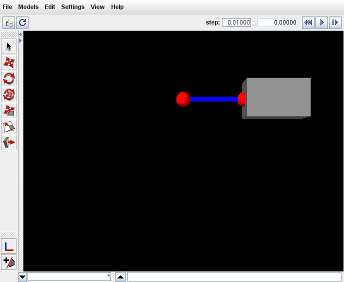
\includegraphics[]{images/RigidBodySpring}
\else
 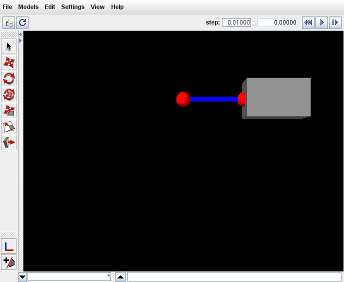
\includegraphics[width=3.75in]{images/RigidBodySpring}
\fi
\end{center}
\caption{RigidBodySpring model loaded into ArtiSynth.}
\label{RigidBodySpring:fig}
\end{figure}

\subsubsection{Example: A simple rigid body-spring model}
\label{RigidBodySpringExample:sec}

A simple rigid body-spring model is defined in
%
\begin{verbatim}
  artisynth.demos.tutorial.RigidBodySpring
\end{verbatim}
%
This differs from ParticleSpring only in the {\tt build()} method,
which is listed below:
\lstset{numbers=left}
\begin{lstlisting}[]
   public void build (String[] args) {

      // create MechModel and add to RootModel
      MechModel mech = new MechModel ("mech");
      addModel (mech);

      // create the components
      Particle p1 = new Particle ("p1", /*mass=*/2, /*x,y,z=*/0, 0, 0);
      // create box and set it's pose (position/orientation):
      RigidBody box =
         RigidBody.createBox ("box", /*wx,wy,wz=*/0.5, 0.3, 0.3, /*density=*/20);
      box.setPose (new RigidTransform3d (/*x,y,z=*/0.75, 0, 0));
      // create marker point and connect it to the box:
      FrameMarker mkr = new FrameMarker (/*x,y,z=*/-0.25, 0, 0);
      mkr.setFrame (box);

      AxialSpring spring = new AxialSpring ("spr", /*restLength=*/0);
      spring.setPoints (p1, mkr);
      spring.setMaterial (
         new LinearAxialMaterial (/*stiffness=*/20, /*damping=*/10));

      // add components to the mech model
      mech.addParticle (p1);
      mech.addRigidBody (box);
      mech.addFrameMarker (mkr);
      mech.addAxialSpring (spring);

      p1.setDynamic (false);               // first particle set to be fixed

      // increase model bounding box for the viewer
      mech.setBounds (/*min=*/-1, 0, -1, /*max=*/1, 0, 0);  
      // set render properties for the components
      RenderProps.setSphericalPoints (p1, 0.06, Color.RED);
      RenderProps.setSphericalPoints (mkr, 0.06, Color.RED);
      RenderProps.setCylindricalLines (mkr, 0.02, Color.BLUE);
   }
\end{lstlisting}
\lstset{numbers=none} 
The differences from {\tt ParticleSpring} begin
at line 9. Instead of creating a second particle, a rigid body is
created using the factory method
\javamethod*[artisynth.core.mechmodels]{RigidBody.createBox()}, which
takes x, y, z widths and a (uniform) density and creates a box-shaped
rigid body complete with surface mesh and appropriate mass and
inertia. As the box is initially centered at the origin, moving it
elsewhere requires setting the body's pose, which is done using {\tt
setPose()}. The {\tt RigidTransform3d} passed to {\tt setPose()} is
created using a three-argument constructor that generates a
translation-only transform.  Next, starting at line 14, a {\tt
FrameMarker} is created for a location $(-0.25, 0, 0)^T$ relative to the
rigid body, and attached to the body using its {\tt setFrame()}
method.

The remainder of {\tt build()} is the same as for {\tt ParticleSpring},
except that the spring is attached to the frame marker instead of a
second particle.

To run this example in ArtiSynth, select {\sf All demos > tutorial >
RigidBodySpring} from the {\sf Models} menu. The model should load and
initially appear as in Figure \ref{RigidBodySpring:fig}.  Running the
model (Section \ref{LoadingAndRunning:sec}) will cause the rigid body
to fall and swing about under gravity.

\subsubsection{Creating rigid bodies}

As illustrated above, rigid bodies can be created using factory
methods supplied by \javaclass[artisynth.core.mechmodels]{RigidBody}.
Some of these include:
%
\begin{lstlisting}[]
  createBox (name, widthx, widthy, widthz, density);
  createCylinder (name, radius, height, density, nsides);
  createSphere (name, radius, density, nslices);
  createEllipsoid (name, radx, rady, radz, density, nslices);
\end{lstlisting}
%
The bodies do not need to be named; if no name is desired, then {\tt
name} and can be specified as {\tt null}.

In addition, there are also
factory methods for creating a rigid body directly from a mesh:
%
\begin{lstlisting}[]
  createFromMesh (name, mesh, density, scale);
  createFromMesh (name, meshFileName, density, scale);
\end{lstlisting}
%
These take either a polygonal mesh (Section \ref{Meshes:sec}), or a
file name from which a mesh is read, and use it as the body's surface
mesh and then compute the mass and inertia properties from the specified
(uniform) density.

Alternatively, one can create a rigid body directly from a
constructor, and then set the mesh and inertia properties explicitly:
%
\begin{lstlisting}[]
  PolygonalMesh femurMesh;
  SpatialInertia inertia;

  ... initialize mesh and inertia appropriately ...

  RigidBody body = new RigidBody ("femur");
  body.setMesh (femurMesh);
  body.setInertia (inertia);
\end{lstlisting}
%

\subsubsection{Pose and velocity}

A body's pose can be set and
queried using the methods
%
\begin{lstlisting}[]
  setPose (RigidTransform3d T);   // sets the pose to T
  getPose (RigidTransform3d T);   // gets the current pose in T
  RigidTransform3d getPose();     // returns the current pose (read-only)
\end{lstlisting}
%
These use a \javaclass[maspack.matrix]{RigidTransform3d} (Section
\ref{RigidTransform3d:sec}) to describe the pose. Body poses are
described in world coordinates and specify the transform from body to
world coordinates. In particular, the pose for a body A specifies
the rigid transform $\T_{AW}$.

Rigid bodies also expose the translational and rotational components of
their pose via the properties {\tt position} and {\tt orientation},
which can be queried and set independently using the methods
%
\begin{lstlisting}[]
  setPosition (Point3d p);       // sets the position to p
  getPosition (Point3d p);       // gets the current position in p
  Point3d getPosition();         // returns the current position (read-only)

  setOrientation (AxisAngle a);  // sets the orientation to a
  getOrientation (AxisAngle a);  // gets the current orientation in a
  AxisAngle getOrientation();    // returns the current orientation (read-only)
\end{lstlisting}
%

The velocity of a rigid body is described using a
\javaclass[maspack.spatialmotion]{Twist} (Section
\ref{SpatialVectors:sec}), which contains both the translational and
rotational velocities. The following methods
set and query the spatial velocity as described with respect to world
coordinates:
%
\begin{lstlisting}[]
  setVelocity (Twist v);         // sets the spatial velocity to v
  getVelocity (Twist v);         // gets the current spatial velocity in v
  Twist getVelocity();           // returns current spatial velocity (read-only)
\end{lstlisting}
%

During simulation, unless a rigid body has been set to be {\it
parametric} (Section \ref{DynamicVsParametric:sec}), its pose and
velocity are updated in response to forces, so setting the pose or
velocity generally makes sense only for setting initial conditions.
On the other hand, if a rigid body is parametric, then it is possible
to control its pose during the simulation, but in that case it is
better to set its {\it target pose} and/or {\it target velocity}, as
described in Section \ref{ControllerImplementation:sec}.

\subsubsection{Inertia and meshes}

The ``mass'' of a rigid body is described by its spatial inertia
(Section \ref{SpatialInertia:sec}), implemented by a
\javaclass[maspack.spatialmotion]{SpatialInertia} object, which
specifies its mass, center of mass, and rotational inertia with
respect to the center of mass.

Most rigid bodies are also associated with a polygonal surface mesh,
which can be set and queried using the methods
%
\begin{lstlisting}[]
  setMesh (PolygonalMesh mesh);
  setMesh (PolygonalMesh mesh, String meshFileName);
  PolygonalMesh getMesh();
\end{lstlisting}
%
The second method takes an optional {\tt fileName} argument that can
be set to the name of a file from which the mesh was read. Then if the
model itself is saved to a file, the model file will specify the mesh
using the file name instead of explicit vertex and face information,
which can reduce the model file size considerably.

The inertia of a rigid body can be explicitly set using a variety
of methods including
%
\begin{lstlisting}[]
  setInertia (M)                    // set using SpatialInertia M
  setInertia (mass, Jxx, Jyy, Jzz); // mass and diagonal rotational inertia
  setInertia (mass, J);             // mass and full rotational inertia
  setInertia (mass, J, com);        // mass, rotational inertia, center-of-mass
\end{lstlisting}
%
and can be queried using 
%
\begin{lstlisting}[]
  getInertia (M);                   // get SpatialInertia in M
  getInertia ();                    // return read-only SpatialInertia
\end{lstlisting}
%

In practice, it is often more convenient to simply specify a mass or a
density, and then use the volume defined by the surface mesh to
compute the remaining inertial values. How a rigid body's inertia is
computed is determined by its {\tt inertiaMethod} property, which can
be one

\begin{description}

\item[Density]\mbox{}

Inertia is computed from density;

\item[Mass]\mbox{}

Inertia is computed from mass;

\item[Explicit]\mbox{}

Inertia is set explicitly.

\end{description}

This property can be set and queried using
%
\begin{lstlisting}[]
  setInertiaMethod (InertiaMethod method);
  InertiaMethod getInertiaMethod();
\end{lstlisting}
%
and its default value is {\tt Density}. Explicitly setting the
inertia using one of {\tt setInertia()} methods described above will
set {\tt inertiaMethod} to {\tt Explicit}. The method
%
\begin{lstlisting}[]
  setInertiaFromDensity (density); 
\end{lstlisting}
%
will (re)compute the inertia using the mesh and a density value
and set {\tt inertiaMethod} to {\tt Density}, and
the method
%
\begin{lstlisting}[]
  setInertiaFromMass (mass); 
\end{lstlisting}
%
will (re)compute the inertia using the mesh and mass value
and set {\tt inertiaMethod} to {\tt Mass}.

Finally, the (assumed uniform) density of the body can be queried
using
%
\begin{lstlisting}[]
   getDensity();
\end{lstlisting}
%

\subsubsection{Damping parameters}
\label{RigidBodyDamping:sec}

As with particles, it is possible to set damping parameters for rigid
bodies. 

{\tt MechModel} provides two properties, {\tt frameDamping} and {\tt
rotaryDamping}, which generate a spatial force centered on each rigid
body's coordinate frame
%
\begin{equation}
\hat\f_i = \matl -d_f \v_i \\ -d_r \Bom_i \matr,
\end{equation}
%
where $d_f$ and $d_r$ are the {\tt frameDamping} and {\tt
rotaryDamping} values, and $\v_i$ and $\Bom_i$ are the translational
and angular velocity of the body's coordinate frame.
The damping parameters can be set and queried using the {\tt MechModel}
methods
%
\begin{lstlisting}[]
  setFrameDamping (double df);
  setRotaryDamping (double dr);
  double getFrameDamping();
  double getRotaryDamping();
\end{lstlisting}
%
\begin{sideblock}
For models involving rigid bodies, it is often necessary to set {\tt
rotaryDamping} to a non-zero value because {\tt frameDamping} will
provide no damping at all when a rigid body is simply rotating about
its coordinate frame origin.
\end{sideblock}

Frame and rotary damping can also be set for individual bodies using
their own (inherited) {\tt frameDamping} and {\tt rotaryDamping}
properties.

\subsection{Joints and connectors}
\label{JointsAndConnectors:sec}

In a typical mechanical model, many of the rigid bodies are
interconnected, either using spring-type components that exert binding
forces on the bodies, or through joint-type connectors that enforce
the connection using hard constraints.

\subsubsection{Joints and coordinate frames}

Consider two bodies A and B. The pose of body B with respect to body A
can be described by the 6 DOF rigid transform $\T_{BA}$.  If bodies A
and B are unconnected, $\T_{BA}$ may assume any possible value
and has a full six degrees of freedom. A {\it joint} between A and B
restricts the set of poses that are possible between the two bodies
and reduces the degrees of freedom available to $\T_{BA}$.  For
simplicity, joints have their own coordinate frames for describing
their constraining actions, and then these frames are related to the
frames A and B of the associated bodies by auxiliary transformations.

\begin{figure}[ht]
\begin{center}
 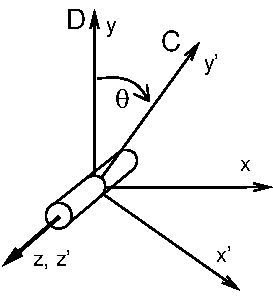
\includegraphics[width=2.5in]{images/jointExample}
\end{center}
\caption{Coordinate frames D and C for a revolute joint.}
\label{jointExample:fig}
\end{figure}

Each joint is associated with two coordinate frames C and D which move
with respect to each other as the joint moves. The allowed joint
motions therefore correspond to the allowed values of the {\it joint transform}
$\T_{CD}$.  D is the {\it base} frame and C is the {\it motion}
frame. For a revolute joint (Figure \ref{jointExample:fig}), C can
move with respect to D by rotating about the z axis. Other motions are
prohibited. $\T_{CD}$ should therefore alway have the form
%
\begin{equation}
\T_{CD} = \matl
\cos(\theta) & -sin(\theta) & 0 \\
\sin(\theta) &  cos(\theta) & 0 \\
0 & 0 & 1\\
\matr
\end{equation}
%
where $\theta$ is the angle of joint rotation and is known as the {\it
joint parameter}. Other joints have different parameterizations, with
the number of parameters equaling the number of degrees of freedom
available to the joint. When $\T_{CD} = \I$ (where $\I$ is the
identity transform), the parameters are all (usually) equal to zero,
and the joint is said to be in the {\it zero state}.

\begin{figure}[ht]
\begin{center}
 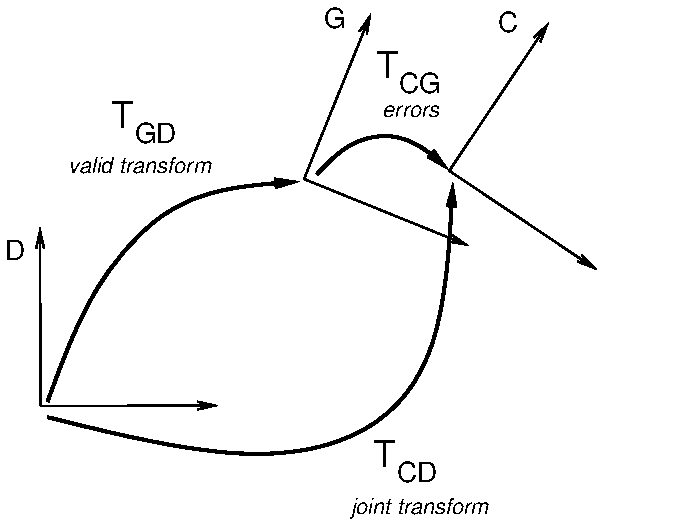
\includegraphics[width=2.5in]{images/jointFrames}
\end{center}
\caption{2D schematic showing the joint frames D and C, along with
the intermediate frame G that accounts for numeric error
and complaint motion.}
\label{jointFrames:fig}
\end{figure}

In practice, due to numerical errors and/or compliance in the joint,
%(Section \ref{JointCompliance:sec}), 
the joint transform $\T_{CD}$ may
sometimes deviate from the allowed set of values dictated by the joint
type. In ArtiSynth, this is accounted for by introducing an additional
{\it constraint} frame G between D and C (Figure \ref{jointFrames:fig}).
G is computed to be the nearest frame to C that lies exactly 
in the joint constraint space. $\T_{GD}$ is therefore a
valid transform for the joint, $\T_{GC}$ accommodates the error,
and the whole joint transform is given by the composition
%
\begin{equation}
\T_{CD} = \T_{GD} \; \T_{CG}.
\end{equation}
%
If there is no compliance or joint error, then frames G and C are the
same, $\T_{CG} = \I$, and $\T_{CD} = \T_{GD}$.

In general, each joint is attached to two rigid bodies A and B, with
frame C being fixed to body A and frame D being fixed to body B. The
restrictions of the joint transform $\T_{CD}$ therefore restrict the
relative poses of A and B.

\begin{figure}[ht]
\begin{center}
 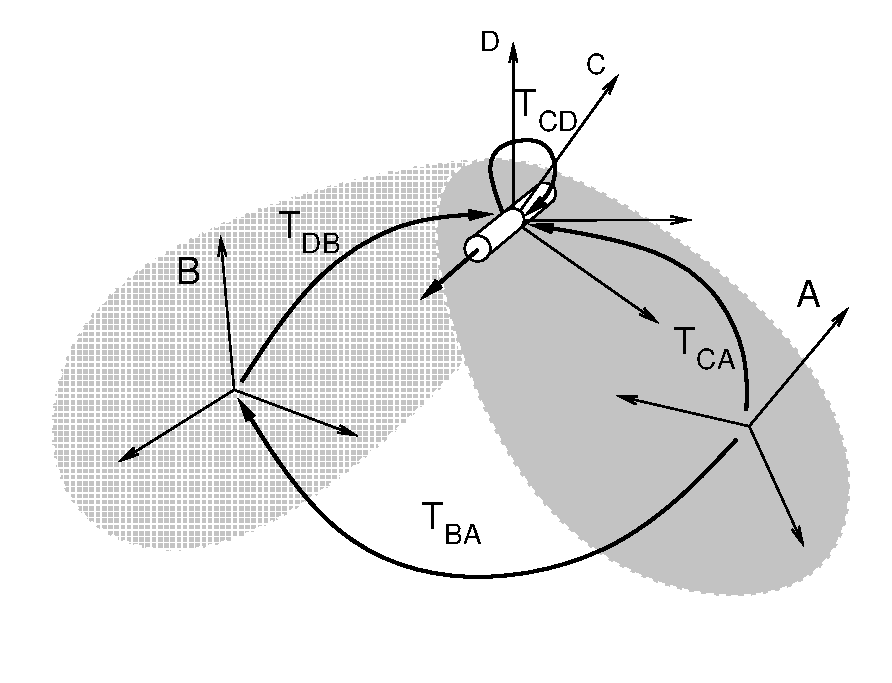
\includegraphics[width=3.74in]{images/jointBodyFrames}
\end{center}
\caption{Transforms connecting joint coordinate frames C and D with
rigid bodies A and B.}
\label{jointBodyFrames:fig}
\end{figure}

Except in special cases, the joint coordinate frames C and D are not
coincident with the body frames A and B.  Instead, they are located
relative to A and B by the transforms $\T_{CA}$ and $\T_{DB}$,
respectively (Figure \ref{jointBodyFrames:fig}). 
Since $\T_{CA}$ and $\T_{DB}$ are both fixed, the pose
of B relative to A can be determined from
the joint transform $\T_{CD}$:
%
\begin{equation}
\T_{BA} = \T_{CA} \, \T_{CD}^{-1} \, \T_{DB}^{-1}.
\label{jointPose:eqn}
\end{equation}
%
(See Section \ref{RigidTransforms:sec} for a discussion of determining
transforms between related coordinate frames).

\subsubsection{Creating Joints}
\label{CreatingJoints:sec}

Joint components in ArtiSynth are implemented by subclasses of
\javaclass[artisynth.core.mechmodels]{RigidBodyConnector}.  Some of
the commonly used ones are described in Section
\ref{CommonJoints:sec}.

An application creates a joint by constructing it and adding it to a
{\tt MechModel}. Most joints generally have a constructor of the form
%
\begin{lstlisting}[]
  JointType (bodyA, bodyB, TDW);
\end{lstlisting}
%
which specifies the rigid bodies A and B which the joint connects,
along with the transform $\T_{DW}$ giving the pose of the joint base
frame D in world coordinates. Then constructor then assumes that the
joint is in the zero state, so that C and D are the same and
$\T_{CD} = \I$ and $\T_{CW} = \T_{DW}$, and then computes
$\T_{CA}$ and $\T_{DB}$ from
%
\begin{align}
\T_{CA} & = \T_{AW}^{-1} \; \T_{CW} \\
\T_{DB} & = \T_{BW}^{-1} \; \T_{DW}
\end{align}
%
where $\T_{AW}$ and $\T_{BW}$ are the poses of A and B.
The same body and transform settings can be made on an existing
joint using the method
\javamethodAlt{%
artisynth.core.mechmodels.RigidBodyConnector.setBodies(,,)}
{setBodies(bodyA, bodyB, TDW)}.

Alternatively, if we prefer to explicitly specify $\T_{CA}$ or $\T_{DB}$, then we
can determine $\T_{DW}$ from $\T_{AW}$ or $\T_{BW}$ using
%
\begin{align}
\T_{DW} & = \T_{AW} \; \T_{CA} \\
\T_{DW} & = \T_{BW} \; \T_{DB}.
\end{align}
%
For example, if we know $\T_{CA}$, this can be accomplished using
the following code fragment:
%
\begin{lstlisting}[]
   RigidBody bodyA, bodyB;
   RigidTransform3d TCA;

   ... initialize bodyA, bodyB, and TCA ...
   
   RigidTransform3d TDW = new RigidTransform3d();
   TDW.mul (bodyA.getPose(), TCA);  // bodyA.getPose() returns TAW
   RevoluteJoint joint = new RevoluteJoint (bodyA, bodyB, TDW);
\end{lstlisting}
%

Another method,
\javamethodAlt{artisynth.core.mechmodels.RigidBodyConnector.setBodies(,,,)}
{setBodies(bodyA, TCA, bodyB, TDB)}, allows us to set both values of
$\T_{CA}$ or $\T_{BA}$ explicitly. This is useful if the joint
transform $\T_{CD}$ is known to be some value {\it other} than the
identity, in which case $\T_{CA}$ or $\T_{BA}$ can be computed
from (\ref{jointPose:eqn}), where $\T_{BA}$ is given by
%
\begin{equation}
\T_{BA} = \T_{AW}^{-1} \; \T_{BW}.
\end{equation}
%
For instance, if we know $\T_{CA}$ and the joint transform $\T_{CD}$,
then we can compute $\T_{DB}$
from
%
\begin{equation}
\T_{DB} = \T_{BA}^{-1} \, \T_{CA} \, \T_{CD}^{-1} = 
\T_{BW}^{-1}  \, \T_{AW} \, \T_{CA} \, \T_{CD}^{-1}
\end{equation}
%
and set up the joint as follows:
%
\begin{lstlisting}[]
   RigidBody bodyA, bodyB;
   RigidTransform3d TCA, TCD;

   ... initialize bodyA, bodyB, TCA, TCD ...
   
   RigidTransform3d TBD = new RigidTransform3d();
   TDB.mulInverseLeft (bodyB.getPose(), bodyA.getPose());
   TDB.mul (TCA);
   TDB.mulInverse (TCD);
   RevoluteJoint joint = new RevoluteJoint ();
   joint.setBodies (bodyA, TCA, bodyB, TDB);
\end{lstlisting}
%

Some joint implementations provide the ability to explicitly set the
joint parameter(s) after it has been created and added to the {\tt
MechModel}, making it easy to ``move'' the joint to a specific
configuration. For example, {\tt RevoluteJoint} provides the method
\javamethod*[artisynth.core.mechmodels.RevoluteJoint]{setTheta()}.
This causes the transform $\T_{CD}$ to be explicitly set to the value
implied by the joint parameters, and the pose of either body A or B is
changed to accommodate this. Whether body A or B is moved depends on
which one is the least connected to ``ground'', and other bodies that have
joint connections to the moved body are moved as well.

If desired, joints can be connected to only a single rigid body. In
this case, the second body B is simply assumed to be ``ground'', and the
coordinate frame B is instead taken
to be the world coordinate frame W. The corresponding calls
to the joint constructor or {\tt setBodies()} take the
form
%
\begin{lstlisting}[]
  JointType joint = new JointType (bodyA, null, TDW);
\end{lstlisting}
%
or
%
\begin{lstlisting}[]
  JointType joint = new JointType();
  joint.setBodies (bodyA, null, TDW);
\end{lstlisting}
%

\subsubsection{Example:  A simple revolute joint}
\label{RigidBodyJoint:sec}

\begin{figure}[ht]
\begin{center}
\iflatexml
 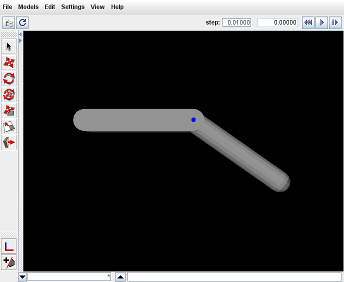
\includegraphics[]{images/RigidBodyJoint}
\else
 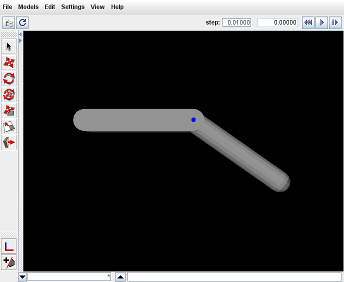
\includegraphics[width=3.75in]{images/RigidBodyJoint}
\fi
\end{center}
\caption{RigidBodyJoint model loaded into ArtiSynth.}
\label{RigidBodyJoint:fig}
\end{figure}

A simple model showing two rigid bodies connected by
a joint is defined in
%
\begin{verbatim}
  artisynth.demos.tutorial.RigidBodyJoint
\end{verbatim}
%

The build method for this model is given below:
\lstset{numbers=left}
\begin{lstlisting}[]
   public void build (String[] args) {

      // create MechModel and add to RootModel
      mech = new MechModel ("mech");
      mech.setGravity (0, 0, -98);
      mech.setFrameDamping (1.0);
      mech.setRotaryDamping (4.0);
      addModel (mech);

      PolygonalMesh mesh;  // bodies will be defined using a mesh

      // create first body and set its pose
      mesh = MeshFactory.createRoundedBox (lenx1, leny1, lenz1, /*nslices=*/8);
      RigidTransform3d TMB = 
         new RigidTransform3d (0, 0, 0, /*axisAng=*/1, 1, 1, 2*Math.PI/3);
      mesh.transform (TMB);
      bodyB = RigidBody.createFromMesh ("bodyB", mesh, /*density=*/0.2, 1.0);
      bodyB.setPose (new RigidTransform3d (0, 0, 1.5*lenx1, 1, 0, 0, Math.PI/2));
      bodyB.setDynamic (false);

      // create second body and set its pose
      mesh = MeshFactory.createRoundedCylinder (
         leny2/2, lenx2, /*nslices=*/16, /*nsegs=*/1, /*flatBottom=*/false);
      mesh.transform (TMB);
      bodyA = RigidBody.createFromMesh ("bodyA", mesh, 0.2, 1.0);
      bodyA.setPose (new RigidTransform3d (
                        (lenx1+lenx2)/2, 0, 1.5*lenx1, 1, 0, 0, Math.PI/2));

      // create the joint      
      RigidTransform3d TDW = 
         new RigidTransform3d (lenx1/2, 0, 1.5*lenx1, 1, 0, 0, Math.PI/2);
      RevoluteJoint joint = new RevoluteJoint (bodyA, bodyB, TDW);

      // add components to the mech model
      mech.addRigidBody (bodyB);
      mech.addRigidBody (bodyA);
      mech.addRigidBodyConnector (joint);

      joint.setTheta (35);  // set joint position

      // set render properties for components
      RenderProps.setLineRadius (joint, 0.2);
      joint.setAxisLength (4);
   }
\end{lstlisting}
\lstset{numbers=none}

A {\tt MechModel} is created as usual at line 4. However, in this
example, we also set some parameters for it:
\javamethod*[artisynth.core.mechmodels.MechModel]{setGravity()} is
used to set the gravity acceleration vector to $(0, 0, -98)^T$ instead
of the default value of $(0, 0, -9.8)^T$, and the {\tt frameDamping}
and {\tt rotaryDamping} properties (Section
\ref{RigidBodyDamping:sec}) are set to provide appropriate damping.

Each of the two rigid bodies are created from a mesh and a density.
The meshes themselves are created using the factory methods
\javamethod*[maspack.geometry]{MeshFactory.createRoundedBox()} and
\javamethod*[maspack.geometry]{MeshFactory.createRoundedCylinder()}
(lines 13 and 22), and then
\javamethod*[artisynth.core.mechmodels]{RigidBody.createFromMesh()} is
used to turn these into rigid bodies with a density of 0.2 (lines 17
and 25). The pose of the two bodies is set using {\tt
RigidTransform3d} objects created with x, y, z translation and
axis-angle orientation values (lines 18 and 26).

The revolute joint is implemented using
\javaclass[artisynth.core.mechmodels]{RevoluteJoint}, which is
constructed at line 32 with the joint coordinate frame D being located
in world coordinates by {\tt TDW} 
as described in Section \ref{CreatingJoints:sec}.

Once the joint is created and added to the {\tt MechModel}, the method
\javamethod*[artisynth.core.mechmodels.RevoluteJoint]{setTheta()} is
used to explicitly set the joint parameter to 35 degrees. The joint
transform $\T_{CD}$ is then set appropriately and {\tt bodyA} is moved
to accommodate this ({\tt bodyA} being chosen since it is the freest
to move).

Finally, render properties are set starting at line 42. A revolute
joint is rendered as a line segment, using the line render properties
(Section \ref{RenderProperties:sec}), with {\tt lineStyle} and {\tt
lineColor} set to {\tt Cylinder} and {\tt BLUE}, respectively, by
default. The cylinder radius and length are specified by the line
render property {\tt lineRadius} and the revolute joint property {\tt
axisLength}, which are set explicitly in the code.

To run this example in ArtiSynth, select {\sf All demos > tutorial >
RigidBodyJoint} from the {\sf Models} menu. The model should load and
initially appear as in Figure \ref{RigidBodyJoint:fig}.  Running the
model (Section \ref{LoadingAndRunning:sec}) will cause {\tt bodyA} to
fall and swing under gravity.

\subsubsection{Commonly used joints}
\label{CommonJoints:sec}

\begin{figure}
\begin{center}
\begin{tabular}{cc}
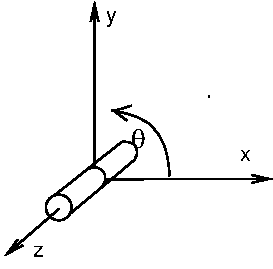
\includegraphics[width=1.75in]{images/revoluteJoint}&
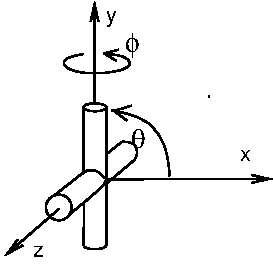
\includegraphics[width=1.75in]{images/rollPitchJoint}\\
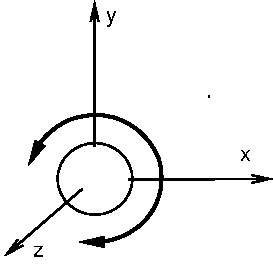
\includegraphics[width=1.75in]{images/sphericalJoint}&
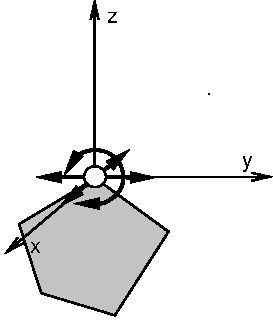
\includegraphics[width=1.75in]{images/planarConnector}\\
\end{tabular}
\end{center}
\caption{Commonly used joints. Clockwise from
top left: revolute, roll-pitch, spherical, planer connector.}
\label{CommonJoints:fig}
\end{figure}

Some of the joints commonly used by ArtiSynth are shown in Figure
\ref{CommonJoints:fig}. Each illustration shows the allowed joint
motion relative to the base coordinate frame D. Clockwise
from the top-left, these joints are:

\begin{description}

\item[Revolute joint]\mbox{}

A one DOF joint which allows rotation by an angle $\theta$ about
the z axis.

\item[Roll-pitch joint]\mbox{}

A two DOF joint, similar to the revolute joint, which allows the
rotation about z to be followed by an additional rotation $\phi$ about
the (new) y axis.

\item[Spherical joint]\mbox{}

A three DOF joint in which the origin remains fixed but any orientation
may be assumed.

\item[Planar connector]\mbox{}

A five DOF joint which connects a point on a single rigid body to a
plane in space. The point may slide freely in the x-y plane, and the
body may assume any orientation about the point.

\end{description}

% LATER \subsubsection{Joint Compliance}
% LATER \label{JointCompliance:sec}

\subsection{Frame springs}
\label{FrameSprings:sec}

Another way to connect two rigid bodies together is to use a {\it
frame spring}, which is a six dimensional spring that generates
restoring forces and moments between coordinate frames.

\subsubsection{Frame spring coordinate frames}

\begin{figure}[ht]
\begin{center}
 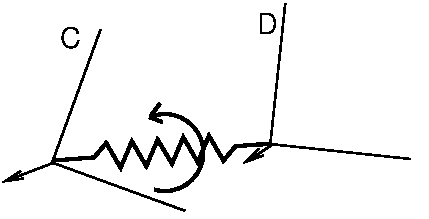
\includegraphics[width=3in]{images/frameSpring}
\end{center}
\caption{A frame spring connecting two coordinate frames D and C.}
\label{frameSpring:fig}
\end{figure}

The basic idea of a frame spring is shown in Figure
\ref{frameSpring:fig}. It generates restoring forces and moments on
two frames C and D which are a function of $\T_{DC}$ and $\hat\v_{DC}$
(the spatial velocity of frame D with respect to frame C).

Decomposing forces into stiffness and damping terms, the force
$\f_C$ and moment $\Btau_C$ acting on C can be expressed as 
%
\begin{align}
\f_C & = \f_{k} (\T_{DC}) + \f_{d} (\hat\v_{DC}) \notag \\
\Btau_C & = \Btau_{k} (\T_{DC}) + \Btau_{d} (\hat\v_{DC}).
\label{ftauC:eqn}
\end{align}
%
where the translational and rotational forces $\f_{k}$, $\f_{d}$,
$\Btau_{k}$, and $\Btau_{d}$ are general functions of $\T_{DC}$ and
$\hat\v_{DC}$.

The forces acting on D are equal and opposite, so that
%
\begin{align}
\f_D & = - \f_C, \notag \\
\Btau_D & = - \Btau_C.
\label{ftau2:eqn}
\end{align}
%

\begin{figure}[ht]
\begin{center}
 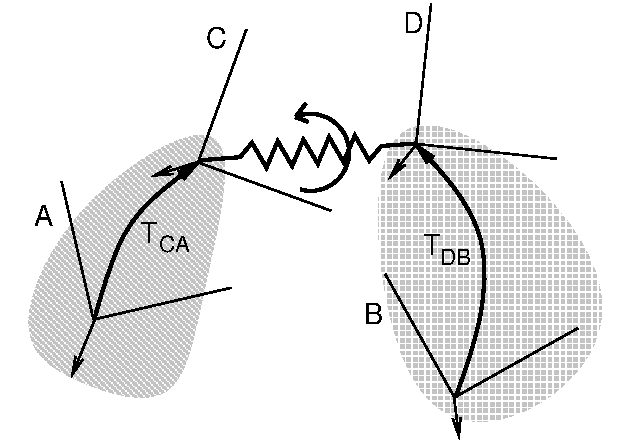
\includegraphics[width=3in]{images/frameSpringBodies}
\end{center}
\caption{A frame spring connecting two rigid bodies A and B.}
\label{frameSpringBodies:fig}
\end{figure}

If frames C and D are attached to a pair of rigid bodies A and B, then
a frame spring can be used to connect them in a manner analogous to a
joint. As with joints, C and D generally do not coincide with the body
frames, and are instead offset from them by fixed transforms $\T_{CA}$
and $\T_{DB}$ (Figure \ref{frameSpringBodies:fig}).

\subsubsection{Frame materials}

The restoring forces (\ref{ftauC:eqn}) generated in a frame spring
depend on the {\it frame material} associated with the spring. Frame
materials are defined in the package {\tt artisynth.core.materials},
and are subclassed from
\javaclass[artisynth.core.materials]{FrameMaterial}.
The most basic type of material is a 
\javaclass[artisynth.core.materials]{LinearFrameMaterial},
in which the restoring forces are determined from
%
\begin{align*}
\f_C & = 
\K_{t} \, \x_{DC} + \D_{t} \, \v_{DC} \\
\Btau_C & = 
\K_{r} \, \hat\Bthe_{DC} + \D_{r} \, \Bom_{DC}
\label{flinear:eqn}
\end{align*}
%
where $\hat\Bthe_{DC}$ gives the small angle approximation of the
rotational components of $\X_{DC}$ with respect to the $x$, $y$, and
$z$ axes, and
%
\begin{gather*}
\K_{t} \equiv 
\matl k_{tx} & 0 & 0 \\ 0 & k_{ty} & 0 \\ 0 & 0 & k_{tz} \matr, \;
\D_{t} \equiv 
\matl d_{tx} & 0 & 0 \\ 0 & d_{ty} & 0 \\ 0 & 0 & d_{tz} \matr, \;\\
\K_{r} \equiv
\matl k_{r x} & 0 & 0 \\ 0 & k_{r y} & 0 \\ 0 & 0 & k_{r z} \matr, \;
\D_{r} \equiv
\matl d_{r x} & 0 & 0 \\ 0 & d_{r y} & 0 \\ 0 & 0 & d_{r z} \matr.
\end{gather*}
%
are the stiffness and damping matrices. The diagonal values defining
each matrix are stored in the 3-dimensional vectors $\k_t$, $\k_r$,
$\d_t$, and $\d_r$ which are exposed as the {\tt stiffness}, {\tt
rotaryStiffness}, {\tt damping}, and {\tt rotaryDamping} properties of
the material. Each of these specifies stiffness or damping values
along or about a particular axis. Specifying different values for
different axes will result in anisotropic behavior.

Other frame materials offering nonlinear behaviour may be defined in
{\tt artisynth.core.materials}.

\subsubsection{Creating frame springs}
\label{CreatingFrameSprings:sec}

Frame springs are implemented by the class
\javaclass[artisynth.core.mechmodels]{FrameSpring}.  Creating a frame
spring generally involves instantiating this class, and then setting
the material, the bodies A and B, and the transforms $\T_{CA}$ and
$\T_{DB}$.

A typical construction sequence might look like this:
%
\begin{lstlisting}[]
  FrameSpring spring = new FrameSpring ("springA");
  spring.setMaterial (new LinearFrameMaterial (kt, kr, dt, dr));
  spring.setFrames (bodyA, bodyB, TDW);
\end{lstlisting}
%
The material is set using
\javamethod*[artisynth.core.mechmodels.FrameSpring]{setMaterial()}.
The example above uses a {\tt LinearFrameMaterial}, created with a
constructor that sets $\k_t$, $\k_r$, $\d_t$, and $\d_r$ to uniform
isotropic values specified by {\tt kt}, {\tt kr}, {\tt dt}, and {\tt
dr}. 

The bodies and transforms can be set in the same manner as for joints
(Section \ref{CreatingJoints:sec}), with the
methods\\ \javamethodAlt{artisynth.core.mechmodels.FrameSpring.setFrames(Frame,Frame,RigidTransform3d)}{setFrames(bodyA,bodyB,TDW)}
and
\javamethodAlt{artisynth.core.mechmodels.FrameSpring.setFrames(Frame,RigidTransform3d,Frame,RigidTransform3d)}{setFrames(bodyA,TCA,bodyB,TDB)}
assuming the role of the {\tt setBodies()} methods used for joints.
The former takes D specified in world coordinates and computes
$\T_{CA}$ and $\T_{DB}$ assuming that there is no initial spring
displacement (i.e., that $\T_{DC} = \I$), while the latter allows
$\T_{CA}$ and $\T_{DB}$ to be specified explicitly with $\T_{DC}$
assuming whatever value is implied.

Frame springs and joints are often placed together, using the same
transforms $\T_{CA}$ and $\T_{DB}$, with the spring providing
restoring forces to help keep the joint within prescribed bounds.

As with joints, a frame spring can be connected to only a single body,
by specifying {\tt frameB} as {\tt null}. Frame B is then taken to be
the world coordinate frame W.

\subsubsection{Example: Two bodies connected by a frame spring}

\begin{figure}[ht]
\begin{center}
\iflatexml
 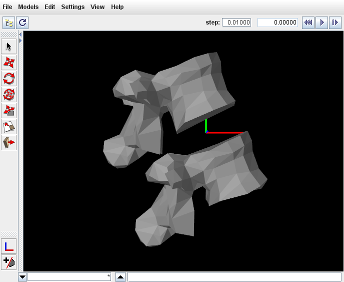
\includegraphics[]{images/LumbarFrameSpring}
\else
 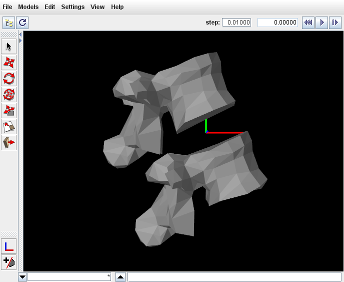
\includegraphics[width=3.75in]{images/LumbarFrameSpring}
\fi
\end{center}
\caption{LumbarFrameSpring model loaded into ArtiSynth.}
\label{LumbarFrameSpring:fig}
\end{figure}

A simple model showing two simplified lumbar vertebrae, modeled as
rigid bodies and connected by a frame spring, is defined in
%
\begin{verbatim}
  artisynth.demos.tutorial.LumbarFrameSpring
\end{verbatim}
%
The definition for the entire model class is shown here:
\lstset{numbers=left}
\lstinputlisting{../../src/artisynth/demos/tutorial/LumbarFrameSpring.java}
\lstset{numbers=none}

For convenience, the code to create and add each vertebrae is wrapped
into the method {\tt addBone()} defined at lines 27-32. This method
takes two arguments: the {\tt MechModel} to which the bone should be
added, and the name of the bone. Surface meshes for the bones are
located in {\tt .obj} files located in the directory {\tt
../mech/geometry} relative to the source directory for the model
itself.
\javamethod*[artisynth.core.util]{ArtisynthPath.getSrcRelativePath()}
is used to find a proper path to this directory given the model class
type ({\tt LumbarFrameSpring.class}), and this is stored in the static
string {\tt geometryDir}. Within {\tt addBone()}, the directory path
and the bone name are used to create a path to the bone mesh itself,
which is in turn used to create a {\tt PolygonalMesh} (line 28). The
mesh is then used in conjunction with a {\tt density} to create a
rigid body which is added to the {\tt MechModel} (lines 29-30) and
returned.

The {\tt build()} method begins by creating and adding a {\tt
MechModel}, specifying a low value for gravity, and setting the rigid
body damping properties {\tt frameDamping} and {\tt
rotaryDamping} (lines 37-41). (The damping parameters are needed
here because the frame spring itself is created with no damping.)
Rigid bodies representing the vertebrae {\tt lumbar1} and {\tt
lumbar2} are then created by calling {\tt addBone()} (lines 44-45),
{\tt lumbar1} is translated by setting the origin of its pose to
$(-0.016, 0.039, 0)^T$, and {\tt lumbar2} is set to be fixed by making
it non-dynamic (line 47).

\begin{figure}[ht]
\begin{center}
\iflatexml
 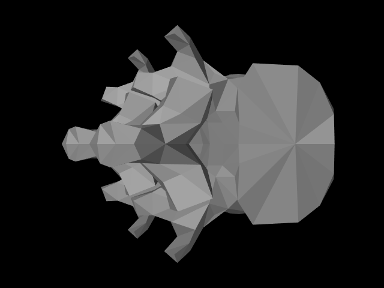
\includegraphics[]{images/LumbarFrameSpringNoflip}
\else
 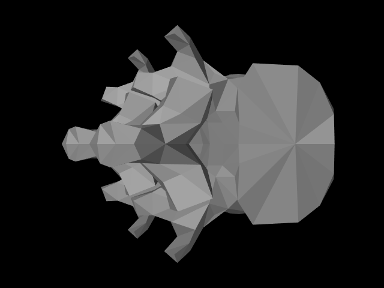
\includegraphics[width=3.75in]{images/LumbarFrameSpringNoflip}
\fi
\end{center}
\caption{LumbarFrameSpring model as it would appear if not rotated
about the x axis.}
\label{LumbarFrameSpringNoflip:fig}
\end{figure}

At this point in the construction, if the model were to be loaded, it
would appear as in Figure \ref{LumbarFrameSpringNoflip:fig}. To change
the viewpoint to that seen in Figure \ref{LumbarFrameSpring:fig}, we
rotate the entire model about the x axis (line 50).  This is done
using
\javamethodAlt{artisynth.core.mechmodels.MechModel.transformGeometry()}
{transformGeometry(X)}, which transforms the geometry of an entire
model using a rigid or affine transform. This method is
described in more detail in Section \ref{TransformingGeometry:sec}.

The frame spring is created and added at lines 54-59, using the
methods described in Section \ref{CreatingFrameSprings:sec}, with
frame D set to the (initial) pose of {\tt lumbar1}.

Render properties are set starting at line 62. By default, a frame
spring renders as a pair of red, green, blue coordinate axes showing
frames C and D, along with a line connecting them. The line width and
the color of the connecting line are controlled by the line render
properties {\tt lineWidth} and {\tt lineColor}, while the length of
the coordinate axes is controlled by the special frame spring property
{\tt axisLength}.

To run this example in ArtiSynth, select {\sf All demos > tutorial >
LumbarFrameSpring} from the {\sf Models} menu. The model should load
and initially appear as in Figure \ref{LumbarFrameSpring:fig}.
Running the model (Section \ref{LoadingAndRunning:sec}) will cause
{\tt lumbar1} to fall slightly under gravity until the frame spring
arrests the motion. To get a sense of the spring's behavior, one can
interactively apply forces to {\tt lumbar1} using the pull manipulator
(see the section ``Pull Manipulator'' in the
\href{../uiguide/uiguide.html}{
ArtiSynth User Interface Guide}).

\subsection{Attachments}
\label{Attachments:sec}

ArtiSynth provides the ability to rigidly attach dynamic components to
other dynamic components, allowing different parts of a model to be
connected together.  Attachments are made by adding to a {\tt
MechModel} special {\it attachment} components that manage the
attachment physics as described briefly in Section
\ref{PhysicsSimulation:sec}.

\subsubsection{Point attachments}
\label{sec:mech:pointattachments}

Point attachments allow particles and other point-based components to
be attached to other, more complex components, such as frames, rigid
bodies, or finite element models (Section \ref{sec:fem:nodeattachments}). Point
attachments are implemented by creating attachment components that are
instances of \javaclass[artisynth.core.mechmodels]{PointAttachment}.
Modeling applications do not generally handle the attachment
components directly, but instead create them implicitly using the
following {\tt MechModel} method:
%
\begin{lstlisting}[]
  attachPoint (Point p1, PointAttachable comp);
\end{lstlisting}
%
This attaches a point {\tt p1} to any component which implements the
interface \javaclass[artisynth.core.mechmodels]{PointAttachable},
indicating that it is capable creating an attachment to a
point. Components that implement {\tt PointAttachable} currently
include rigid bodies, particles, and finite element models. The
attachment is created based on the the current position of the point
and component in question.  For attaching a point to a rigid body,
another method may be used:
%
\begin{lstlisting}[]
  attachPoint (Point p1, RigidBody body, Point3d loc);
\end{lstlisting}
%
This attaches {\tt p1} to {\tt body} at the point {\tt loc} specified
in body coordinates.  Finite element attachments are discussed in
Section \ref{sec:fem:nodeattachments}.

Once at point is attached, it
will be in the {\it attached} state, as described in Section
\ref{DynamicVsParametric:sec}.  Attachments can be removed by
calling
%
\begin{lstlisting}[]
  detachPoint (Point p1);   
\end{lstlisting}
%

\subsubsection{Example: model with particle attachments}

\begin{figure}[ht]
\begin{center}
\iflatexml
 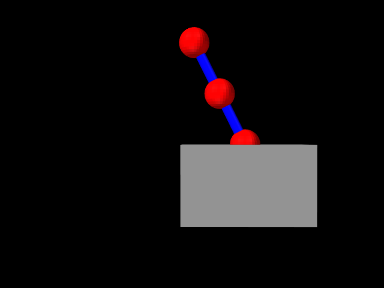
\includegraphics[]{images/ParticleAttachment}
\else
 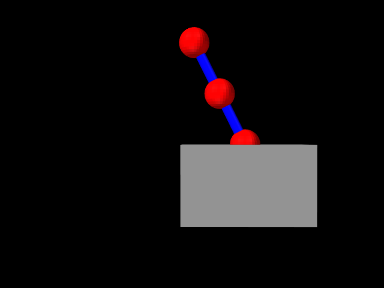
\includegraphics[width=3.75in]{images/ParticleAttachment}
\fi
\end{center}
\caption{ParticleAttachment model loaded into ArtiSynth.}
\label{ParticleAttachment:fig}
\end{figure}

A model illustrating particle-particle and particle-rigid body attachments
is defined in
%
\begin{verbatim}
  artisynth.demos.tutorial.ParticleAttachment
\end{verbatim}
%
and most of the code is shown here:
%
\lstset{numbers=left}
\begin{lstlisting}[]
   public Particle addParticle (MechModel mech, double x, double y, double z) {
      // create a particle at x, y, z and add it to mech
      Particle p = new Particle (/*name=*/null, /*mass=*/.1, x, y, z);
      mech.addParticle (p);
      return p;
   }

   public AxialSpring addSpring (MechModel mech, Particle p1, Particle p2){
      // create a spring connecting p1 and p2 and add it to mech
      AxialSpring spr = new AxialSpring (/*name=*/null, /*restLength=*/0);
      spr.setMaterial (new LinearAxialMaterial (/*k=*/20, /*d=*/10));
      spr.setPoints (p1, p2);
      mech.addAxialSpring (spr);
      return spr;
   }

   public void build (String[] args) {

      // create MechModel and add to RootModel
      MechModel mech = new MechModel ("mech");
      addModel (mech);

      // create the components
      Particle p1 = addParticle (mech, 0, 0, 0.55);
      Particle p2 = addParticle (mech, 0.1, 0, 0.35);
      Particle p3 = addParticle (mech, 0.1, 0, 0.35);
      Particle p4 = addParticle (mech, 0, 0, 0.15);
      addSpring (mech, p1, p2);
      addSpring (mech, p3, p4);
      // create box and set its pose (position/orientation):
      RigidBody box =
         RigidBody.createBox ("box", /*wx,wy,wz=*/0.5, 0.3, 0.3, /*density=*/20);
      box.setPose (new RigidTransform3d (/*x,y,z=*/0.2, 0, 0));
      mech.addRigidBody (box);

      p1.setDynamic (false);               // first particle set to be fixed

      // set up the attachments
      mech.attachPoint (p2, p3);
      mech.attachPoint (p4, box, new Point3d (0, 0, 0.15));

      // increase model bounding box for the viewer
      mech.setBounds (/*min=*/-0.5, 0, -0.5, /*max=*/0.5, 0, 0);  
      // set render properties for the components
      RenderProps.setSphericalPoints (mech, 0.06, Color.RED);
      RenderProps.setCylindricalLines (mech, 0.02, Color.BLUE);
   }
\end{lstlisting}
\lstset{numbers=none}
%
The code is very similar to {\tt ParticleSpring} and {\tt
RigidBodySpring} described in Sections \ref{ParticleSpringExample:sec}
and \ref{RigidBodySpringExample:sec}, except that two convenience
methods, {\tt addParticle()} and {\tt addSpring()}, are defined at
lines 1-15 to create particles and spring and add them to a {\tt
MechModel}. These are used in the {\tt build()} method to create four
particles and two springs (lines 24-29), along with a rigid body box
(lines 31-34). As with the other examples, particle {\tt p1} is set to
be non-dynamic (line 36) in order to fix it in place and provide a
ground.

The attachments are added at lines 39-40, with {\tt p2} attached to
{\tt p3} and {\tt p4} connected to the box at the location $(0, 0,
0.15)$ in box coordinates. 

Finally, render properties are set starting at line 43. In this
example, point and line render properties are set for the entire {\tt
MechModel} instead of individual components.  Since render properties
are inherited, this will implicitly set the specified render
properties in all sub-components for which these properties are not
explicitly set (either locally or in an intermediate ancestor).

To run this example in ArtiSynth, select {\sf All demos > tutorial >
ParticleAttachment} from the {\sf Models} menu. The model should load
and initially appear as in Figure \ref{ParticleAttachment:fig}.
Running the model (Section \ref{LoadingAndRunning:sec}) will cause the
box to fall and swing under gravity.

\subsubsection{Frame attachments}
\label{sec:mech:frameattachments}

Frame attachments allow rigid bodies and other frame-based components to
be attached to other components, including frames, rigid
bodies, or finite element models (Section \ref{sec:fem:frameattachments}).
Frame attachments are implemented by creating attachment components that are
instances of \javaclass[artisynth.core.mechmodels]{FrameAttachment}.

As with point attachments, modeling applications do not generally
handle frame attachment components directly, but instead create and
add them
implicitly using the following {\tt MechModel} methods:
%
\begin{lstlisting}[]
  attachFrame (Frame frame, FrameAttachable comp);

  attachFrame (Frame frame, FrameAttachable comp, RigidTransform3d TFW);
\end{lstlisting}
%
These attach {\tt frame} to any component which implements the
interface \javaclass[artisynth.core.mechmodels]{FrameAttachable},
indicating that it is capable of creating an attachment to a
frame. Components that implement {\tt FrameAttachable} currently
include frames, rigid bodies, and finite element models.  For the
first method, the attachment is created based on the the current
position of the frame and component in question. For the second
method, the attachment is created so that the initial pose of the frame
(in world coordinates) is described by {\tt TFW}.

Once a frame is attached, it
will be in the {\it attached} state, as described in Section
\ref{DynamicVsParametric:sec}.  Frame attachments can be removed by
calling
%
\begin{lstlisting}[]
  detachFrame (Frame frame);   
\end{lstlisting}
%

\begin{sideblock}
While it is possible to create composite rigid bodies using {\tt
FrameAttachments}, this is much less computationally efficient (and
less accurate) than creating a single rigid body through mesh merging
or similar techniques.
\end{sideblock}

\subsubsection{Example: model with frame attachments}

\begin{figure}[ht]
\begin{center}
\iflatexml
 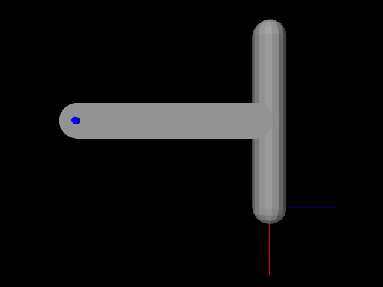
\includegraphics[]{images/FrameBodyAttachment}
\else
 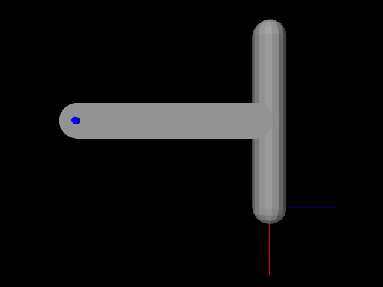
\includegraphics[width=3.75in]{images/FrameBodyAttachment}
\fi
\end{center}
\caption{FrameBodyAttachment model loaded into ArtiSynth.}
\label{FrameBodyAttachment:fig}
\end{figure}

A model illustrating rigidBody-rigidBody and frame-rigidBody attachments
is defined in
%
\begin{verbatim}
  artisynth.demos.tutorial.FrameBodyAttachment
\end{verbatim}
%
Most of the code is identical to that for {\tt RigidBodyJoint}
as described in Section \ref{RigidBodyJoint:sec}, except that
the joint is further to the left and connects {\tt bodyB} to ground,
rather than to {\tt bodyA}, and the initial pose of {\tt bodyA}
is changed so that it is aligned vertically. {\tt bodyA} is
then connected to {\tt bodyB}, and an auxiliary frame is created
and attached to {\tt bodyA}, using code at the end
of the {\tt build()} method as shown here:
%
\lstset{numbers=left}
\begin{lstlisting}[]
   public void build (String[] args) {

      ... create model mostly similar to RigidBodyJoint ...

      // now connect bodyA to bodyB using a FrameAttachment
      mech.attachFrame (bodyA, bodyB);

      // create an auxiliary frame and add it to the mech model
      Frame frame = new Frame();
      mech.addFrame (frame);
      
      // set the frames axis length > 0 so we can see it
      frame.setAxisLength (4.0); 
      // set the attached frame's pose to that of bodyA ...
      RigidTransform3d TFW = new RigidTransform3d (bodyA.getPose());
      // ... plus a translation of lenx2/2 along the x axis:
      TFW.mulXyz (lenx2/2, 0, 0);
      // finally, attach the frame to bodyA
      mech.attachFrame (frame, bodyA, TFW);
   }
\end{lstlisting}
\lstset{numbers=none}
%
To run this example in ArtiSynth, select {\sf All demos > tutorial >
FrameBodyAttachment} from the {\sf Models} menu. The model should load
and initially appear as in Figure \ref{ParticleAttachment:fig}.  The
frame attached to {\tt bodyA} is visible in the lower right corner.
Running the model (Section \ref{LoadingAndRunning:sec}) will cause
both bodies to fall and swing about the joint under gravity.



%!TEX root = modelguide.tex

\section{Mechanical Models II}
\label{MechModelsII:sec}

This section provides additional material on building basic
multibody-type mechanical models.

\subsection{Simulation control properties}

Both \javaclass[artisynth.core.workspace]{RootModel} and
\javaclass[artisynth.core.mechmodels]{MechModel} contain properties
that control the simulation behavior. One of the most important of
these is {\tt maxStepSize}. By default, simulation proceeds using the
{\tt maxStepSize} value defined for the root model. A {\tt MechModel}
(or any other type of {\tt Model}) contained in the root model's {\tt
models} list may also request a smaller step size by specifying a
smaller value for its own {\tt maxStepSize} property.  For all models,
the {\tt maxStepSize} may be set and queried using
%
\begin{lstlisting}[]
  void setMaxStepSize (double maxh);
  double getMaxStepSize();
\end{lstlisting}
%

Another important simulation property is {\tt integrator} in {\tt
MechModel}, which determines the type of integrator used for the
physics simulation. The value type of this property is the enumerated
type {\tt MechSystemSolver.Integrator}, for which the following values
are currently defined:

\begin{description}

\item[ForwardEuler]\mbox{}

First order forward Euler integrator. Unstable for stiff systems.

\item[SymplecticEuler]\mbox{}

First order symplectic Euler integrator, more energy conserving
that forward Euler. Unstable for stiff systems.

\item[RungeKutta4]\mbox{}

Fourth order Runge-Kutta integrator, quite accurate but also unstable
for stiff systems.

\item[ConstrainedBackwardEuler]\mbox{}

First order backward order integrator. Generally stable for stiff systems.

\item[Trapezoidal]\mbox{}

Second order trapezoidal integrator. Generally stable for stiff
systems, but slightly less so than {\tt ConstrainedBackwardEuler}.

\end{description}

The term ``Unstable for stiff systems'' means that the integrator is
likely to go unstable in the presence of ``stiff'' systems, which
typically include systems containing finite element models, unless the
simulation step size is set to an extremely small value.  The default
value for {\tt integrator} is {\tt ConstrainedBackwardEuler}.

\begin{sideblock}
Stiff systems tend to arise in models containing interconnected
deformable elements, for which the step size should not exceed the
propagation time across the smallest element, an effect known as the
Courant-Friedrichs-Lewy (CFL) condition. Larger stiffness and damping
values decrease the propagation time and hence the allowable step
size.
\end{sideblock}

Another {\tt MechModel} simulation property is {\tt stabilization},
which controls the stabilization method used to correct drift from
position constraints and correct interpenetrations due to collisions.
The value type of this property value is the enumerated type {\tt
MechSystemSolver.PosStabilization}, which presently has two values:

\begin{description}

\item[GlobalMass]\mbox{}

Uses only a diagonal mass matrix for the MLCP that is solved to
determine the position corrections. This is the default method.

\item[GlobalStiffness]\mbox{}

Uses a stiffness-corrected mass matrix for the MLCP that is solved to
determine the position corrections. Slower than {\tt GlobalMass}, but
more likely to produce stable results, particularly for
problems involving FEM collisions.

\end{description}

\subsection{Units}
\label{sec:mechii:units}

ArtiSynth is primarily ``unitless'', in the sense that it does not
define default units for the fundamental physical quantities of time,
length, and mass. Although time is
generally understood to be in seconds, and often declared as such in
method arguments and return values, there is no hard requirement that
it be interpreted as seconds. There are no assumptions at all
regarding length and mass. Some components may have default parameter
values that reflect a particular choice of units, such as {\tt
MechModel}'s default gravity value of $(0, 0, -9.8)^T$, which is
associated with the MKS system, but these values can always be
overridden by the application.

Nevertheless, it is important, and up to the application developer to
ensure, that units be {\it consistent}. For example, if one decides to
switch length units from meters to centimeters (a common choice),
then all units involving length will have to be scaled appropriately.
For example, density, whose fundamental units are $m/d^3$, where $m$ is mass and
$d$ is distance, needs to be scaled by $1/100^3$, or $0.000001$, when
converting from meters to centimeters.

Table \ref{Units:tab} lists a number of common physical quantities
used in ArtiSynth, along with their associated fundamental units.

\begin{table}
\begin{center}
\begin{tabular}{|lll|}
\hline
unit & fundamental units & \\
\hline
time                    & $t$ & \\
distance                & $d$ & \\
mass                    & $m$ & \\
velocity                & $d/t$ & \\
acceleration            & $d/t^2$ & \\
force                   & $m d/t^2$ & \\
work/energy             & $m d^2/t^2$& \\
torque                  & $m d^2/t^2$ & same as energy (somewhat counterintuitive)\\
angular velocity        & $1/t$ & \\
angular acceleration    & $1/t^2$ & \\
rotational inertia      & $m d^2$ & \\
pressure                & $m/(d t^2)$ & \\
Young's modulus         & $m/(d t^2)$ & \\
Poisson's ratio         & 1 & no units; it is a ratio \\
density                 & $m/d^3$ & \\
linear stiffness        & $m/t^2$ & \\
linear damping          & $m/t$ & \\
rotary stiffness        & $m d^2/t^2$ & same as torque \\
rotary damping          & $m d^2/t$ & \\
mass damping            & $1/t$ & used in FemModel \\
stiffness damping       & $t$ & used in FemModel \\
\hline
\end{tabular}
\end{center}
\caption{Physical quantities and their representation in terms of the
fundamental units of mass ($m$), distance ($d$), and time ($t$).}
\label{Units:tab}
\end{table}

\subsubsection{Scaling units}

For convenience, many ArtiSynth components, including {\tt MechModel},
implement the interface
\javaclass[artisynth.core.util]{ScalableUnits}, which
provides the following methods for scaling mass and distance units:
%
\begin{lstlisting}[]
  scaleDistance (s);    // scale distance units by s
  scaleMass (s);        // scale mass units by s
\end{lstlisting}
%
A call to one of these methods should cause all physical quantities
within the component (and its descendants) to be
scaled as required by the fundamental unit relationships
as shown in Table \ref{Units:tab}.

Converting a {\tt MechModel} from meters to centimeters can therefore be
easily done by calling 
%
\begin{lstlisting}[]
   mech.scaleDistance (100);
\end{lstlisting}
%
As an example, adding the following code to the end of the {\tt build()}
method in {\tt RigidBodySpring} (Section \ref{RigidBodySpringExample:sec})
%
\begin{lstlisting}[]
   System.out.println ("length=" + spring.getLength());
   System.out.println ("density=" + box.getDensity());
   System.out.println ("gravity=" + mech.getGravity());
   mech.scaleDistance (100);
   System.out.println ("");
   System.out.println ("scaled length=" + spring.getLength());
   System.out.println ("scaled density=" + box.getDensity());
   System.out.println ("scaled gravity=" + mech.getGravity());
\end{lstlisting}
%
will scale the distance units by 100 and print the values of various
quantities before and after scaling. The resulting output is:
%
\begin{lstlisting}[]
   length=0.5
   density=20.0
   gravity=0.0 0.0 -9.8

   scaled length=50.0
   scaled density=2.0E-5
   scaled gravity=0.0 0.0 -980.0
\end{lstlisting}
%

\begin{sideblock}
It is important not to confuse scaling units with scaling the actual
geometry or mass. Scaling units should change all physical
quantities so that the simulated behavior of the model remains
unchanged.  If the distance-scaled version of {\tt RigidBodySpring}
shown above is run, it should behave exactly the same as the
non-scaled version.
\end{sideblock}

%\subsection{Multi-point springs}
%OPTIONAL
%\subsubsection{Operation}
%\subsubsection{Example: A single multi-point spring}

%\begin{figure}[ht]
%\begin{center}
%\iflatexml
% 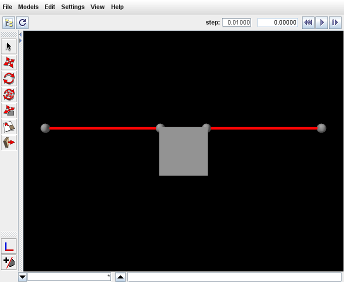
\includegraphics[]{images/MultiPointSpring}
%\else
% 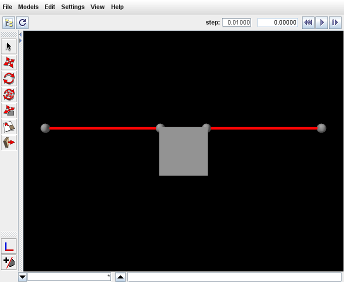
\includegraphics[width=3.75in]{images/MultiPointSpring}
%\fi
%\end{center}
%\caption{MultiPointSpring model loaded into ArtiSynth.}
%\label{MultiPointSpring:fig}
%\end{figure}
%
%A simple model showing a multi-point spring is defined in
%%
%\begin{verbatim}
%  artisynth.demos.tutorial.MultiPointSpring
%\end{verbatim}
%

% MultiPointSpring

\subsection{Render properties}
\label{RenderProperties:sec}

All ArtiSynth components that are renderable maintain a property {\tt
renderProps}, which stores a
\javaclass[maspack.render]{RenderProps} object that contains a number
of subproperties used to control an object's rendered appearance.

In code, the {\tt renderProps} property for an object can be set or
queried using the methods
%
\begin{lstlisting}[]
  setRenderProps (RenderProps props); // set render properties
  RenderProps getRenderProps();       // get render properties (read-only)
\end{lstlisting}
%
Render properties can also be set in the GUI by selecting one or more
components and the choosing {\sf Set render props ...}  in the
right-click context menu. More details on setting render properties
through the GUI can be found in the section ``Render properties'' in the
\href{../uiguide/uiguide.html}{
ArtiSynth User Interface Guide}.

For many components, the default value of {\tt renderProps} is {\tt
null}; i.e., no {\tt RenderProps} object is assigned by default and
render properties are instead inherited from ancestor components
further up the hierarchy. The reason for this is because {\tt
RenderProps} objects are fairly large (many kilobytes), and so
assigning a unique one to every component could consume too much
memory. Even when a {\tt RenderProps} object is assigned, most of its
properties are inherited by default, and so only those properties
which are explicitly set will differ from those specified in ancestor
components.

\subsubsection{Render property taxonomy}

In general, the properties in {\tt RenderProps} are used to control
the color, size, style, and resolution of the three primary rendering
primitives: faces, lines, and points. Table \ref{RenderProps:tab}
contains a complete list. Values for the {\tt shading}, {\tt
faceStyle}, {\tt lineStyle} and {\tt pointStyle} properties are
defined using the enumerated types {\tt RenderProps.Shading}, {\tt
RenderProps.Faces}, {\tt RenderProps.LineStyle}, and {\tt
RenderProps.PointStyle}.  Colors are specified using {\tt
java.awt.Color}.

\begin{table}
\begin{center}
\begin{tabular}{|lll|}
\hline property & purpose & usual default value \\ \hline
%Generic properties:
visible & whether or not the component is visible & {\tt true} \\
alpha & transparency for polygonal faces (range 0 to 1) & 1 (opaque) \\
shading & polygon shading: ({\tt FLAT}, {\tt GOURARD}, {\tt PHONG}) & {\tt FLAT}\\
shininess & shininess parameter for polygons (range 0 to 32) & 32 \\
%Face related properties &
\hline
faceStyle &
which polygonal faces are drawn ({\tt FRONT}, {\tt BACK},
{\tt FRONT\_AND\_BACK}, {\tt NONE}) & {\tt FRONT} \\
faceColor &
color used for drawing faces & {\tt GREY} \\
backColor &
color used for drawing backs of faces. If {\tt null}, {\tt faceColor} is used. &
{\tt null} \\
drawEdges & if true, polygon edges are drawn explicitly & {\tt false} \\
% Edge related properties &
\hline
edgeColor & color for edges & {\tt GREY} \\
edgeWidth & edge width in pixels & 1 \\
% Line related properties &
\hline
lineStyle: &
how lines are drawn ({\tt CYLINDER}, {\tt LINE}, or {\tt ELLIPSOID}) & 
{\tt LINE} \\
lineColor & color for lines & {\tt GREY} \\
lineWidth & width in pixels when {\tt LINE} style is selected & 1 \\
lineRadius & radius when {\tt CYLINDER} or {\tt ELLIPSOID} style is selected &
1 \\
lineSlices &
number of slices used to render {\tt CYLINDER} or {\tt ELLIPSOID} style lines &
32 \\
% Point related properties &
\hline
pointStyle & how points are drawn ({\tt SPHERE} or {\tt POINT}) & {\tt POINT} \\
pointColor & color for points & {\tt GREY} \\
pointSize & point size in pixels when {\tt POINT} style is selected & 1 \\
pointRadius & sphere radius when {\tt SPHERE} style is selected & 1 \\
pointSlices & number of slices used to render {\tt SPHERE} style spheres & 32 \\
\hline
\end{tabular}
\end{center}
\caption{Render properties and their default values.}
\label{RenderProps:tab}
\end{table}

To increase and improve their visibility, both the line and point
primitives are associated with styles ({\tt CYLINDER}, {\tt
ELLIPSOID}, and {\tt SPHERE}) that allow them to be rendered using 3D
surface geometry.

Exactly how a component interprets its render properties is up to the
component (and more specifically, up to the rendering method for that
component).  Not all render properties are relevant to all components,
particularly if the rendering does not use all of the rendering
primitives. For example,
\javaclass[artisynth.core.mechmodels]{Particle} components use only
the point primitives and
\javaclass[artisynth.core.mechmodels]{AxialSpring} components use only
the line primitives. For this reason, some components use subclasses
of {\tt RenderProps}, such as
\javaclass[maspack.render]{PointRenderProps} and
\javaclass[maspack.render]{LineRenderProps}, that expose only a subset
of the available render properties. All renderable components provide
the method
\javamethod[maspack.render.HasRenderProps]{createRenderProps()} that
will create and return a {\tt RenderProps} object suitable for that
component.

\subsubsection{Setting render properties}
\label{SettingRenderProperties:sec}

When setting render properties, it is important to note that
the value returned by
\javamethod[maspack.render.HasRenderProps]{getRenderProps()} 
should be treated as {\it read-only} and should {\it not}
be used to set property values.
For example, applications should {\it not} do the
following:
\begin{lstlisting}[]
   particle.getRenderProps().setPointColor (Color.BLUE);
\end{lstlisting}
%
This can cause problems for two reasons. First, {\tt getRenderProps()}
will return {\tt null} if the object does not currently have a {\tt
RenderProps} object. Second, because {\tt RenderProps} objects are
large, ArtiSynth may try to share them between components, and so by
setting them for one component, the application my inadvertently set
them for other components as well.

Instead, {\tt RenderProps} provides a static method for each property
that can be used to set that property's value for a specific
component.  For example, the correct way to set {\tt pointColor} is
%
\begin{lstlisting}[]
   RenderProps.setPointColor (particle, Color.BLUE);
\end{lstlisting}
%

One can also set render properties by calling
\javamethod*[maspack.render.HasRenderProps]{setRenderProps()} with a
predefined {\tt RenderProps} object as an argument. This is useful for
setting a large number of properties at once:
%
\begin{lstlisting}[]
   RenderProps props = new RenderProps();
   props.setPointColor (Color.BLUE);
   props.setPointRadius (2);
   props.setPointStyle (RenderProps.PointStyle.SPHERE);

   ...

   particle.setRenderProps (props);
\end{lstlisting}

\begin{sideblock}
Note that even though components may use a subclass of {\tt
RenderProps} internally, one can always use the base {\tt RenderProps}
class to set values; properties which are not relevant to the
component will simply be ignored.
\end{sideblock}

Finally, as mentioned above, render properties are inherited.  Values
set high in the component hierarchy will be inherited by descendant
components, unless those descendants (or intermediate components)
explicitly set overriding values.  For example, a {\tt MechModel}
maintains its own {\tt RenderProps} (and which is never null). Setting
its {\tt pointColor} property to {\tt RED} will cause {\it all}
point-related components within that {\tt MechModel} to be rendered as
red {\it except} for components that set their {\tt pointColor} to a
different property.

There are typically three levels in a {\tt MechModel} component
hierarchy at which render properties can be set:

\begin{itemize}

\item The {\tt MechModel} itself;

\item Lists containing components;

\item Individual components.

\end{itemize}

For example, consider the following code:
%
\begin{lstlisting}[]
   MechModel mech = new MechModel ("mech");

   Particle p1 = new Particle (/*name=*/null, 2, 0, 0, 0);
   Particle p2 = new Particle (/*name=*/null, 2, 1, 0, 0);
   Particle p3 = new Particle (/*name=*/null, 2, 1, 1, 0);

   mech.addParticle (p1);
   mech.addParticle (p2);
   mech.addParticle (p3);

   RenderProps.setPointColor (mech, Color.BLUE);
   RenderProps.setPointColor (mech.particles(), Color.GREEN);
   RenderProps.setPointColor (p3, Color.RED);   
\end{lstlisting}
%
Setting the {\tt MechModel} render property {\tt pointColor} to {\tt
BLUE} will cause all point-related items to be rendered blue by
default. Setting the {\tt pointColor} render property for the particle
list (returned by {\tt mech.particles()}) will override this and cause
all particles in the list to be rendered green by default. Lastly,
setting {\tt pointColor} for {\tt p3} will cause it to be rendered as
red.

\subsection{Point-to-point muscles}
\label{PointToPointMuscles:sec}

Point-to-point muscles are a simple type of component in biomechanical
models that provide muscle-activated forces acting along a line
between two points. ArtiSynth provides this through
\javaclass[artisynth.core.mechmodels]{Muscle}, which is a subclass of
\javaclass[artisynth.core.mechmodels]{AxialSpring} that generates an
active muscle force in response to its {\tt
excitation} property. The excitation property can be set and queried
using the methods
%
\begin{lstlisting}[]
   setExcitation (double a);
   double getExcitation();
\end{lstlisting}
%

\subsubsection{Muscle materials}
\label{sec:mechii:musclematerials}

As with {\tt AxialSpring}s, {\tt Muscle} components use an
\javaclass[artisynth.core.materials]{AxialMaterial} to compute the
applied force $f (l, \dot l, a)$ in response to the muscle's length
$l$, length velocity $\dot l$, and excitation signal $a$.  Usually the
force is the sum of a {\it passive} component plus an {\it active}
component that arises in response to the excitation signal.

The default {\tt AxialMaterial} for a {\tt Muscle} is
\javaclass[artisynth.core.materials]{SimpleAxialMuscle},
which is essentially an activated version of 
\javaclass[artisynth.core.materials]{LinearAxialMaterial}
and 
which computes a simple force according to
%
\begin{equation}
f(l, \dot l) = k (l-l_0) + d \dot l + m_f a
\end{equation}
%
where $k$ and $d$ are stiffness and damping terms, $a$ is the
excitation value, and $m_f$ is the maximum excitation force.
$k$, $d$ and $m_f$ are exposed through the properties {\tt
stiffness}, {\tt damping}, and {\tt maxForce}.

More complex muscle materials are typically used for biomechanical
modeling applications, generally with non-linear passive terms and
active terms that depend on the muscle length $l$.  Some of those
available in ArtiSynth include
\javaclass[artisynth.core.materials]{ConstantAxialMuscle},
\javaclass[artisynth.core.materials]{BlemkerAxialMuscle},
\javaclass[artisynth.core.materials]{PaiAxialMuscle}, and
\javaclass[artisynth.core.materials]{PeckAxialMuscle}.

% LATER: describe muscles in more detail

\subsubsection{Example: Muscle attached to a rigid body}
\label{SimpleMuscleExample:sec}

\begin{figure}[ht]
\begin{center}
\iflatexml
 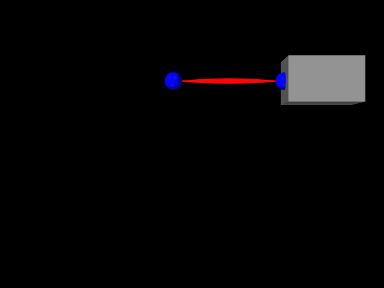
\includegraphics[]{images/SimpleMuscle}
\else
 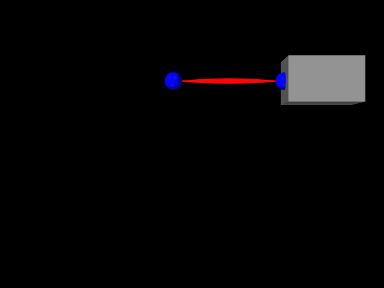
\includegraphics[width=3.75in]{images/SimpleMuscle}
\fi
\end{center}
\caption{SimpleMuscle model loaded into ArtiSynth.}
\label{SimpleMuscle:fig}
\end{figure}

A simple model showing a single muscle connected to a rigid
body is defined in
%
\begin{verbatim}
  artisynth.demos.tutorial.SimpleMuscle
\end{verbatim}
%

This model is identical to {\tt RigidBodySpring} described in Section
\ref{RigidBodySpringExample:sec}, except that the code to create
the spring is replaced with code to create a muscle
with a {\tt SimpleAxialMuscle} material:
%
\begin{lstlisting}[]
      // create the muscle:      
      muscle = new Muscle ("mus", /*restLength=*/0);
      muscle.setPoints (p1, mkr);
      muscle.setMaterial (
         new SimpleAxialMuscle (/*stiffness=*/20, /*damping=*/10, /*maxf=*/10));
\end{lstlisting}
%
Also, so that the muscle renders differently, the rendering style
for lines is set to {\tt ELLIPSOID} using the convenience method
%
\begin{lstlisting}[]
      RenderProps.setEllipsoidalLines (muscle, 0.02, Color.RED);
\end{lstlisting}
%

To run this example in ArtiSynth, select {\sf All demos > tutorial >
SimpleMuscle} from the {\sf Models} menu. The model should load and
initially appear as in Figure \ref{SimpleMuscle:fig}.  Running the
model (Section \ref{LoadingAndRunning:sec}) will cause the box to fall
and sway under gravity. To see the effect of the {\tt excitation}
property, select the muscle in the viewer and then choose {\sf Edit
properties ...} from the right-click context menu.  This will open an
editing panel that allows the muscle's properties to be adjusted
interactively. Adjusting the {\tt excitation} property using the
adjacent slider will cause the muscle force to vary.

% LATER \subsubsection{Multi-point muscles}

% LATER \subsection{Mesh components}
%OPTIONAL 
% LATER \subsubsection{Fixed meshes}
% LATER \subsubsection{Simple mesh example}

% SimpleMesh

% LATER \subsubsection{Skinned meshes}
% LATER \subsubsection{Simple skinned mesh example}

% SimpleSkinnedMesh

\subsection{Collision Handling}
\label{sec:mechii:collisions}

Collision handling in ArtiSynth is implemented by a collision
handling mechanism build into {\tt MechModel}. Collisions are
disabled by default, but can be enabled between rigid and deformable
bodies (finite element models in particular), and more generally
between any body that implements the interface 
\javaclass[artisynth.core.mechmodels]{Collidable}.

It is important to understand that collison handling is both
computationally expensive and, due to it's discontinuous nature, less
accurate than other aspects of the simulation.  ArtiSynth therefore
provides a number of ways to selectively control collision handling
between different pairs of bodies.

%\subsubsection{Collidable bodies}

\subsubsection{Enabling collisions in code}

Collisions can be enabled as either a default behavior between all
bodies, a default behavior between certain {\it types} of
bodies, or a specific behavior between individual pairs of bodies.

The default collision behavior between all collidables can be
controlled using two equivalent methods:
%
\begin{lstlisting}[]
  setDefaultCollisionBehavior (enabled, mu);
  setDefaultCollisionBehavior (behavior);
\end{lstlisting}
%
where {\tt enabled} is {\tt true} or {\tt false} depending on whether
collisions are enabled, {\tt mu} is the coefficient of Coulomb (or
dry) friction, and {\tt behavior} is a
\javaclass[artisynth.core.mechmodels]{CollisionBehavior} object that
specifies both {\it enabled} and {\it mu}. The {\tt mu} value is
ignored if {\tt enabled} is {\tt false}.  In addition, collisions can
be controlled for specific {\it types} of collidables using
%
\begin{lstlisting}[]
  setDefaultCollisionBehavior (typeA, typeB, enabled, mu);
  setDefaultCollisionBehavior (typeA, typeB, behavior);
\end{lstlisting}
%
where {\tt typeA} and {\tt typeB} should be either {\tt
Collidable.RigidBody} or {\tt Collidable.Deformable}.  In addition,\\
{\tt Collidable.Deformable} can be paired with {\tt Collidable.Self} to
enable/disable self-collisions between deformable objects.
Self-collision is described in greater detail in Section
\ref{SelfCollision:sec}.

A call to one of the {\tt setDefaultCollisionBehavior()} methods will
override the effects of previous calls. So for instance, the code
sequence
%
\begin{lstlisting}[]
  setDefaultCollisionBehvaior (true, 0);
  setDefaultCollisionBehvaior (
    Collidable.Deformable, Collidable.RigidBody, false, 0);
  setDefaultCollisionBehavior (true, 0.2);
\end{lstlisting}
%
will initially enable collisions between all bodies with a friction
coefficient of 0, then {\it disable} collisions between deformable and
rigid bodies, and finally re-enable collisions between all bodies with
a friction coefficient of 0.2.

The default collision behavior between any pair of body types can
be queried using
%
\begin{lstlisting}[]
  CollisionBehavior getDefaultCollisionBehavior (typeA, typeB);
\end{lstlisting}
%

In addition to default behaviors, collisions between individual
collidables can be controlled and queried using
%
\begin{lstlisting}[]
  setCollisionBehavior (collidableA, collidableB, enabled, mu);
  setCollisionBehavior (collidableA, collidableB, behavior);
  getCollisionBehavior (collidableA, collidableB);
\end{lstlisting}
%
where {\tt collidableA} and {\tt collidableB} are individual
collidable components such as rigid bodies or FEM models.  Collision
behaviors specified by {\tt setCollisionBehavior()} {\it override} the
default collision behaviors, and are {\it not} invalidated by
subsequent calls to the {\tt setDefaultCollisionBehavior()} methods.
An overide collision behavior for a specific pair of collidables
can be removed by
%
\begin{lstlisting}[]
  clearCollisionBehavior (collidableA, collidableB);
\end{lstlisting}
%
and {\it all} override behaviors in a {\tt MechModel} can
be removed by 
%
\begin{lstlisting}[]
  clearCollisionBehaviors ();
\end{lstlisting}
%

\begin{sideblock}
Note: It is usually necessary to ensure that collisions are {\it disabled}
between adjacent bodies connected by joints, since otherwise these
would be forced into a state of permanent collision.
\end{sideblock}

\subsubsection{Example: Collision with a plane}
\label{JointedCollide:sec}

\begin{figure}[ht]
\begin{center}
\iflatexml
 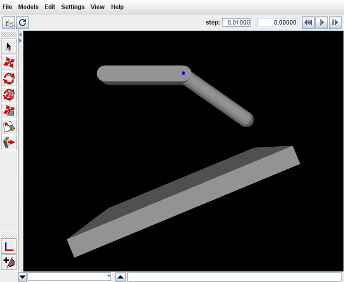
\includegraphics[]{images/JointedCollide}
\else
 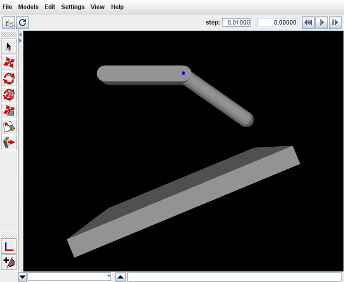
\includegraphics[width=3.75in]{images/JointedCollide}
\fi
\end{center}
\caption{JointedCollide model loaded into ArtiSynth.}
\label{JointedCollide:fig}
\end{figure}

A simple model illustrating collision between two jointed rigid bodies
and a plane is defined in
%
\begin{verbatim}
  artisynth.demos.tutorial.JointedCollide
\end{verbatim}
%

This model is simply a subclass of {\tt RigidBodyJoint} that
overrides the {\tt build()} method 
to add an inclined plane and enable collisions between it and
the two connected bodies:
%
\lstset{numbers=left}
\begin{lstlisting}[]
   public void build (String[] args) {

      super.build (args);

      bodyB.setDynamic (true);  // allow bodyB to fall freely

      // create and add the inclined plane
      RigidBody base = RigidBody.createBox ("base", 25, 25, 2, 0.2);
      base.setPose (new RigidTransform3d (5, 0, 0, 0, 1, 0, -Math.PI/8));
      base.setDynamic (false);
      mech.addRigidBody (base);

      // turn on collisions
      mech.setDefaultCollisionBehavior (true, 0.20);
      mech.setCollisionBehavior (bodyA, bodyB, false);
   }
\end{lstlisting}
\lstset{numbers=none}

The superclass {\tt build()} method called at line 3 creates
everything contained in {\tt RigidBodyJoint}. The remaining code then
alters that model: {\tt bodyB} is set to be dynamic (line 5) so that
it will fall freely, and an inclined plane is created from a thin box
that is translated and rotated and then set to be be non-dynamic
(lines 8-11).  Finally, collisions are enabled by setting the default
collision behavior (line 14), and then specifically disabling
collisions between {\tt bodyA} and {\tt bodyB} (line 15). As indicated
above, the latter step is necessary because the joint would otherwise
keep the two bodies in a permanent state of collision.

To run this example in ArtiSynth, select {\sf All demos > tutorial >
JointedCollide} from the {\sf Models} menu. The model should load and
initially appear as in Figure \ref{JointedCollide:fig}.  Running
the model (Section \ref{LoadingAndRunning:sec}) will
cause the jointed assembly to collide with and slide off the inclined
plane.


\subsubsection{Self-collision and collidable hierarchies}
\label{SelfCollision:sec}

At present, {\tt ArtiSynth} does not support the detection or handling
of self-collision within single meshes. However, self-collision can
still be effected by allowing a collidable to have multiple
{\it sub-collidables} and then enabling collisions between some or all of
these.

Any descendant component of a
\javaclass[artisynth.core.mechmodels]{Collidable} component A which is
itself {\tt Collidable} is considered to be a sub-collidable of A.
Certain types of components maintain sub-collidables by default.  For
example, some components (such as finite element models; Section
\ref{FEMModels:sec}) maintain a list of meshes in a child component
list named {\tt meshes}; these can be used to implement self-collision
as described below.

\begin{sideblock}
Note: A collidable does not need to be an immediate child component
of a collidable A in order to be a sub-collidable of A;
it need only be a descendent of A. 
\end{sideblock}

\begin{figure}[ht]
\begin{center}
 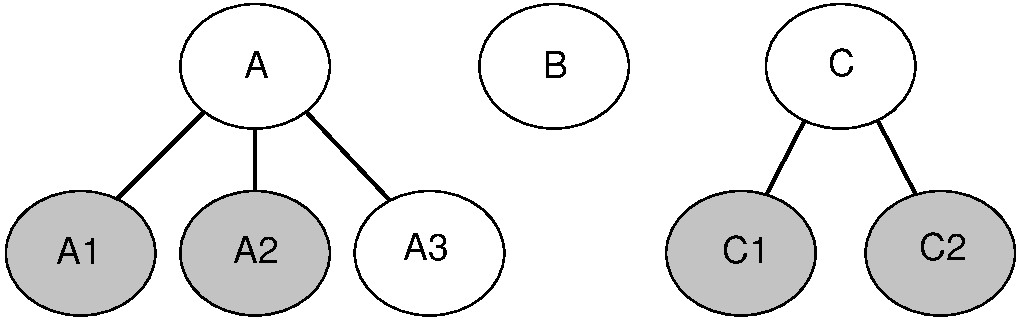
\includegraphics[width=5in]{images/CollidableGroups}
\end{center}
\caption{A collection of collidable components, where A possesses
sub-collidables A1, A2, and A3, B is solitary, and C possesses
sub-collidables C1 and C2. Internal collisions are enabled among those
sub-collidables which are shaded grey.}
\label{CollidableGroups:fig}
\end{figure}

In general, an ArtiSynth model will contain a collection of
collidables, some of which posses sub-collidables and others which are
solitary (Figure \ref{CollidableGroups:fig}).  Within a collection of
collidables:

\begin{itemize}

\item Actual collisions happen only between leaf collidables; ancestor
collidables are used only for grouping purposes.

\item By default, the sub-collidables of a component A will only
collide among themselves if self-collision is specified for A (via
either a default or override collision behavior). If self-collision is
specified for A, then collisions may occur only among those
sub-collidables for which {\it internal} collisions are enabled.
Internal collisions are enabled for a collidable if its {\tt
collidable} property (Section \ref{collidability:sec}) is set to
either {\tt ALL} or {\tt INTERNAL}.

\item Self-collision is also only possible among the sub-collidables
of A if A is itself deformable; i.e., its
\javamethod[artisynth.core.mechmodels.Collidable]{isDeformable()}
method returns {\tt true}.

\item Sub-collidables may collide with collidables outside their
hierarchy if their {\tt collidable} property is set to either {\tt
ALL} or {\tt EXTERNAL}.

\item Collision among specific pairs of sub-collidables may also be
explicitly enabled or disabled with an override behavior set using one
of the {\tt setCollisionBehavior()} methods.

\item Specifying a collision behavior among two collidables A and B
which are {\it not} within the same hierarchy will cause that behavior
to be specified among all sub-collidables of A and B whose {\tt
collidable} property enables the collision.

\end{itemize}

This is best illustrated with some examples. Refer to Figure
\ref{CollidableGroups:fig}, assume that components A, B and C are
deformable, and that self-collision is allowed among those
sub-collidables which are shaded grey (A1 and A2 for A, B1 and B2 for
B). Then:
%
\begin{lstlisting}[]
   // Set default collision among deformable components with friction = 0.2:
   setDefaultCollisionBehavior (
      Collidable.DEFORMABLE, Collidable.DEFORMABLE, true, 0.2);
   // Collisions are now enabled between A1, A2, and A3 and each of B, C1, and
   // C2, and between B and C1 and C2, but not among A1, A2, and A3 or C1 and C2.

   // Enable self-collision between A1 and A2 and B1 and B2 with friction = 0:
   setDefaultCollisionBehavior (Collidable.DEFORMABLE, Collidable.SELF, true, 0);
    
   // Specifically disable collision between B and A3:
   setCollisionBehavior (B, A3, false);

   // Specifically enable collision between A3 and C with friction = 0.3:
   setCollisionBehavior (A3, C, true, 0.3);
   // This behavior will be applied between A3 and each of C1 and C2.

   // Disable self-collision within A:
   setCollisionBehavior (A, A, false);
   // This will disable all self-collisions among A1, A2 and A3.
\end{lstlisting}
%

\subsubsection{Collidability}
\label{collidability:sec}

Each collidable component maintains a {\tt collidable} property
(which can be queried using
\javamethod[artisynth.core.mechmodels.Collidable]{getCollidable()})
which specifically enables or disables the ability of that collidable
to collide with other collidables.

The {\tt collidable} property value is of the enumerated type
\javaclass[artisynth.core.mechmodels]{Collidable\#Collidability}, which
has four possible settings:

\begin{description}

\item[OFF]\mbox{}

All collisions disabled: the collidable will not collide with
anything.

\item[INTERNAL]\mbox{}

Internal (self) collisions enabled: the collidable may only collide
with other Collidables with which it shares a common ancestor.

\item[EXTERNAL]\mbox{}

External collisions enabled: the collidable may only collide with
other Collidables with which it does {\it not} share a common
ancestor.

\item[ALL]\mbox{}

All collisions (both self and external) enabled: the collidable may
collide with any other Collidable.

\end{description}

Note that collidability only {\it enables} collisions.  In order for
collisions to actually occur between two collidables, a default or
override collision behavior must also be specified for them in the
MechModel.

\subsubsection{Implementation and limitations}

The ArtiSynth collision mechanism works by finding intersections
between the surface meshes of each collidable object.  These surface
meshes must (at present) be triangular, closed, and manifold.
A bounding-box 
hierarchy is used to determine if any two surfaces meshes
intersect. If they do, then a tracing algorithm
is used to compute all the intersection contours
between the two meshes as shown in Figure~\ref{Collision:fig}.

\begin{figure}[ht]
\begin{center}
        \begin{tabular}{ccc}
        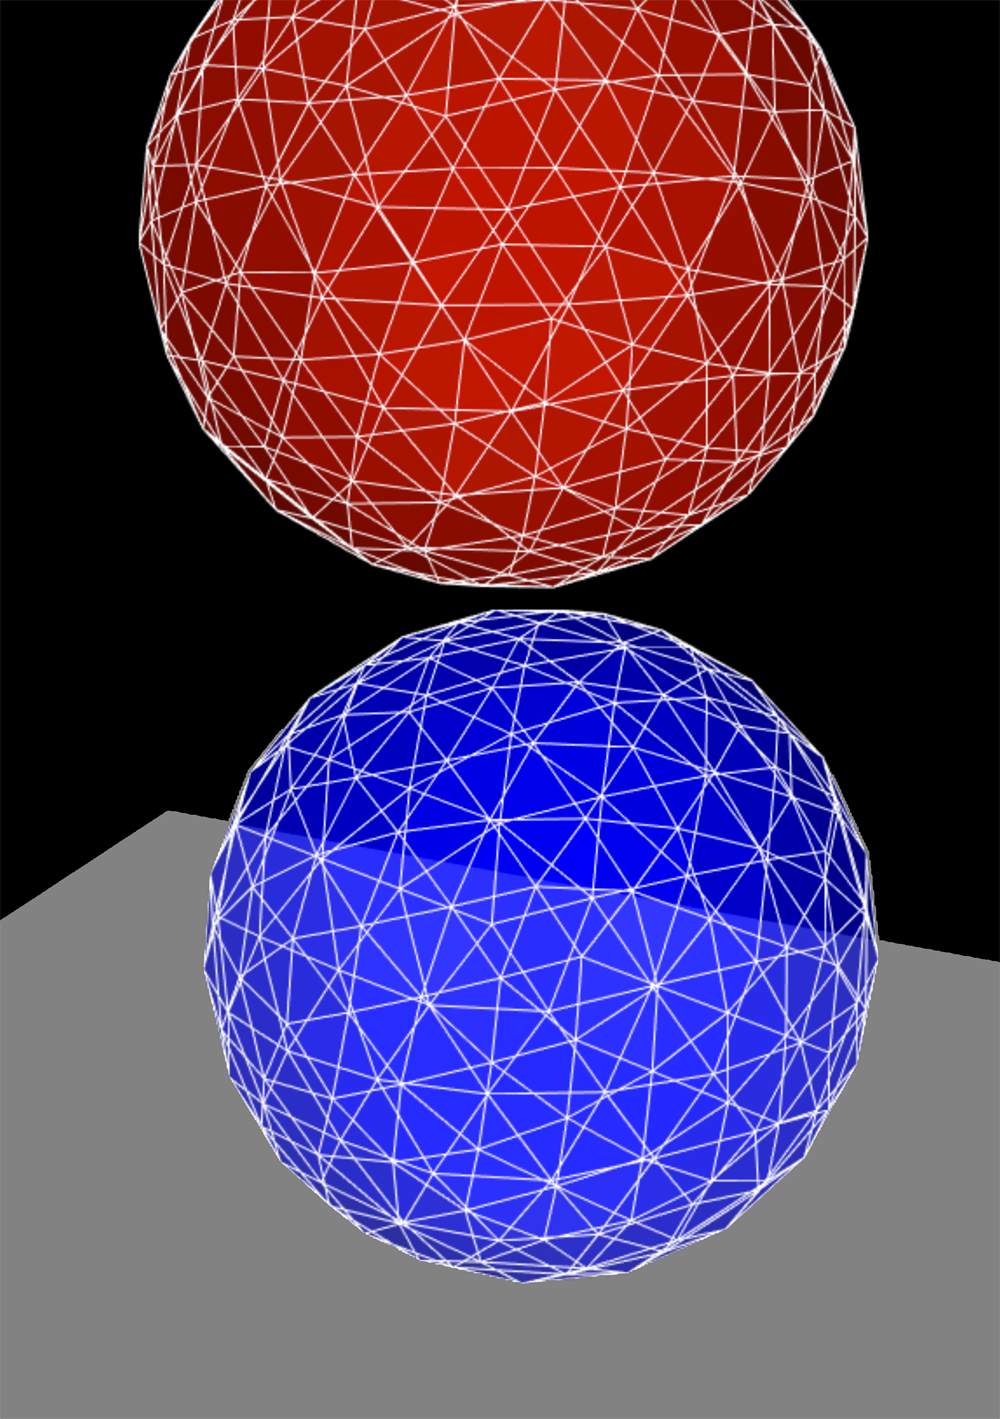
\includegraphics[width=0.31\textwidth]{images/femCollide1} &
        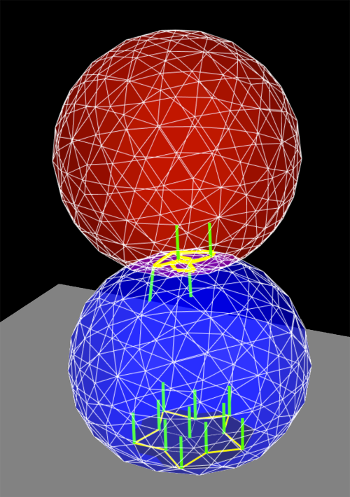
\includegraphics[width=0.31\textwidth]{images/femCollide2} &
        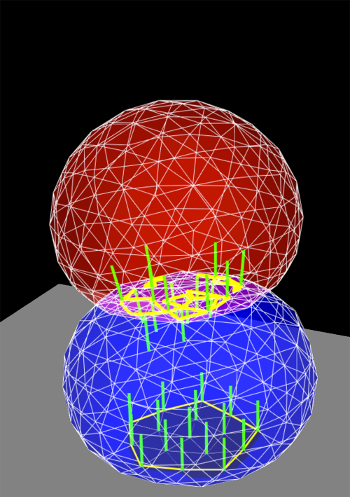
\includegraphics[width=0.31\textwidth]{images/femCollide3}\\
%       \end{tabular}
%       \begin{tabular}{p{1.2cm}p{3.5cm}p{3.5cm}p{3.5cm}} 
         \large  $\mathrm{t}=0$s & \large $\mathrm{t}=0.25$s & \large $\mathrm{t}=0.5$s         
        \end{tabular}
\end{center}
\caption{Time sequence of contact handling between two deformable models 
falling under gravity, 
showing the intersection contours
(yellow) and the contact normals (green lines).}
\label{Collision:fig}
\end{figure}

% XXX -useAjlCollision and contours?

Determining the intersection contour allows us to create a set of
constraints for correcting the interpenetration and preventing
interpenetrating velocities.  For rigid bodies, this is done by
fitting a plane to each contour, projecting the contour onto this
plane, and then sampling the vertices of the projection's 2D convex
hull to create individual contact points, with the contact normal set
from the normal of the plane. For deformable FEM models, the
intersection contour is used to locate all the interpenetrating nodes,
and then collision constraints are established between each node and
the nearest triangular face of the opposing surface.

Because ArtiSynth currently uses static collision detection, it is
possible for objects that are fast enough or thin enough to completely
pass through each other in one simulation step. This means that for
thin objects, it is important to keep the step size small enough to
prevent such undetected interpenetration.

ArtiSynth also uses a ``box'' friction approximation
\cite{Lacoursiere07} to compute dry friction, instead of the
polyhedralized friction cones common in the multibody dynamics
literature \cite{AnitescuPotra2002,PotraEtAlTrapezoidal2006}.  This
allows for a less expensive and more robust computation at the expense
of some accuracy.

Another issue is that ArtiSynth's attempt to separate colliding bodies
at the end of each time step may cause a jittering behavior around the
colliding area, as the surface collides, separates, and re-collides.
This can usually be stabilized by maintaining a certain
interpenetration distance during contact. This distance is controlled
by the {\tt MechModel} property {\tt penetrationTol}.  ArtiSynth
attempts to compute a suitable default value for this property, but
for some applications it may be necessary to control the value
explicitly using the {\tt MechModel} methods
%
\begin{lstlisting}[]
   setInterpenetrationTol (double dist);
   double getInterpenetrationTol();
\end{lstlisting}
%

Other aspects of collision handling can be adjusted by directly
setting properties of the {\tt MechModel}'s collision manager, which
can be accessed graphically via the navigation panel, or in code using
\javamethod*[artisynth.core.mechmodels.MechModel]{getCollisionManager()}.

One of these properties is {\tt collisionPointTol}, which for
collisions between rigid bodies specifies a minimum distance between
contact points and therefore can be used to reduce the number of
contact constraints and improve computation time.

\subsubsection{Contact rendering}

The {\tt MechModel}'s collision manager component contains render
properties that can be used to render the contact points, normals, and
mesh intersection contours associated with contact.

By default, contact and contour rendering is disabled. To enable it,
one can use the following code fragment:
%
\begin{verbatim}
  RenderProps.setVisible (mechModel.getCollisionManager(), true);
\end{verbatim}
%
The following render properties are used:

\begin{description}

\item[lineStyle] \mbox{}
Style of the line used for rendering the contact normals

\item[lineWidth] \mbox{}
Width (in pixels) of the contact normal if the {\tt Line} line style is used

\item[lineRadius] \mbox{}
Radius of the contact normal if a solid line style is used

\item[lineSlices] \mbox{}
Number of slices in the contact normal for a solid line style

\item[lineColor] \mbox{}
Color of the contact normal

\item[edgeWidth] \mbox{}
Width (in pixels) of the line used to render the contour

\item[edgeColor] \mbox{}
Color of the contour

\end{description}

These properties can be set in the same way as the visibility, using
the {\tt RenderProps} methods presented in Section
\ref{SettingRenderProperties:sec}:

\begin{lstlisting}[]
  Renderable colManager = mechModel.getCollisionManager();
  RenderProps.setEdgeWidth (col, 2);
  RenderProps.setEdgeColor (col, Color.Red);
\end{lstlisting}

To access these properties on a read-only basis, one can do
  
\begin{lstlisting}[]
  RenderProps props = mechModel.getCollisionManager().getRenderProps();
\end{lstlisting}

Finally, to set the length of the rendered contact normals, set the
{\tt contactNormalLen} property in collision manager. Since contact
normals have no preferred direction, it may be necessary to use a
negative length value in order to visualize them properly.

A simple model showing a contact rendering is defined in
%
\begin{verbatim}
  artisynth.demos.tutorial.BallPlateCollide
\end{verbatim}
%
and the complete source code is shown below:
%
\lstset{numbers=left}
\lstinputlisting{../../src/artisynth/demos/tutorial/BallPlateCollide.java}
\lstset{numbers=none}

To run this example in ArtiSynth, select {\sf All demos > tutorial >
BallPlateCollide} from the {\sf Models} menu. When run, the ball
will collide with the plate and the contact normals and collision 
contours with be draw and shown in Figure \ref{BallPlateCollide:fig}.

\begin{figure}[ht]
\begin{center}
\iflatexml
 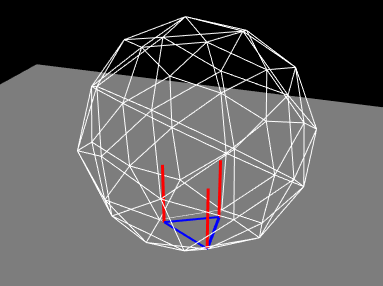
\includegraphics[]{images/BallPlateCollide}
\else
 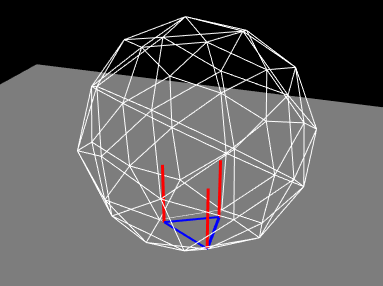
\includegraphics[width=3.75in]{images/BallPlateCollide}
\fi
\end{center}
\caption{BallPlateCollide showing contact normals (red) and collision contour
(blue) of the ball colliding with the plate.}
\label{BallPlateCollide:fig}
\end{figure}

\subsection{Transforming geometry}
\label{TransformingGeometry:sec}

Certain ArtiSynth components, including {\tt MechModel}, implement the
interface \javaclass[artisynth.core.modelbase]{TransformableGeometry},
which allows the geometric transformation of the component's
attributes (such as meshes, points, frame locations, etc.), along with
its descendant components. The interface provides the method
%
\begin{lstlisting}[]
   public void transformGeometry (AffineTransform3dBase X);
\end{lstlisting}
%
where {\tt X} is an \javaclass[maspack.matrix]{AffineTransform3dBase}
that may be either a \javaclass[maspack.matrix]{RigidTransform3d} or a
more general \javaclass[maspack.matrix]{AffineTransform3d} (Section
\ref{RigidTransform3d:sec}).

\javamethodAlt{artisynth.core.modelbase.TransformableGeometry.transformGeometry()}%
{transformGeometry(X)}
can be used to translate, rotate, shear or scale components. It
can be applied to an entire model or individual components. Unlike
\javamethod*[artisynth.core.util.ScalableUnits]{scaleDistance()}, it
actually changes the physical geometry and so may change the
simulation behaviour. For example, applying {\tt transformGeometry()}
to a \javaclass[artisynth.core.mechmodels]{RigidBody} will cause the
shape of its mesh to change, which will change its mass if its {\sf
inertiaDensity} property is set to {\sf Density}.
Figure \ref{RigidAndAffineTransforms:fig} shows a simplified
illustration of both rigid and affine transformations being applied to
a model.

\begin{figure}[ht]
\begin{center}
   \begin{tabular}{ccc}
   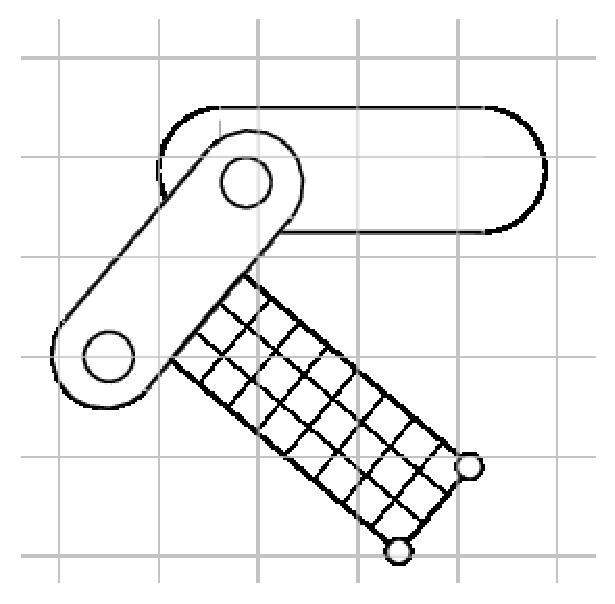
\includegraphics[width=0.27\textwidth]{images/tgenModel} &
   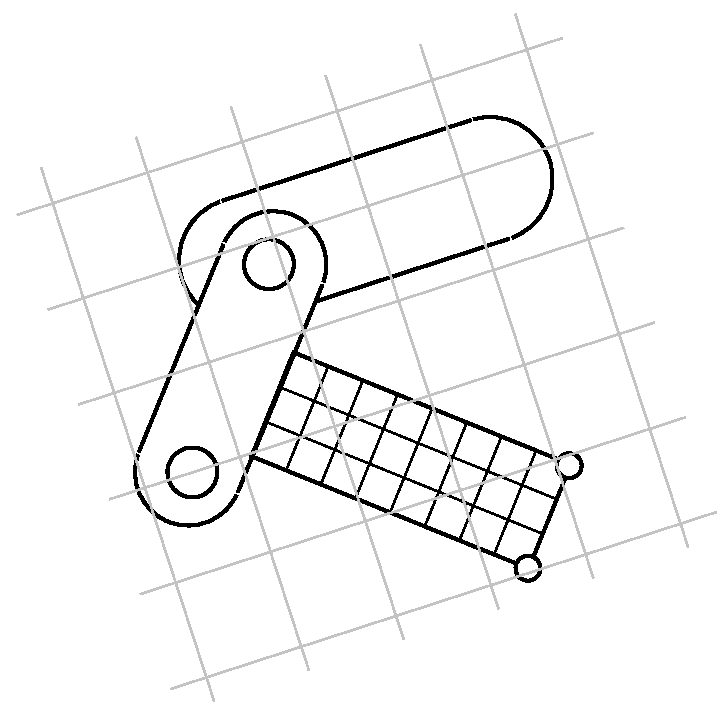
\includegraphics[width=0.34\textwidth]{images/tgenModelRigid} &
   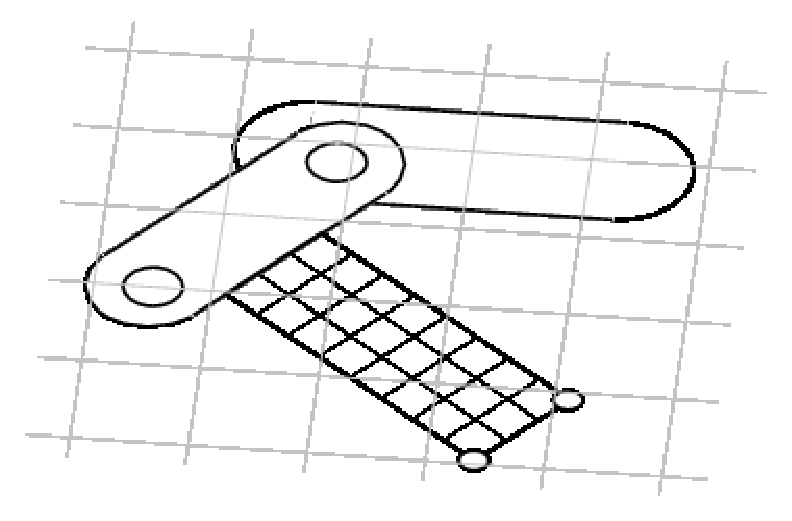
\includegraphics[width=0.34\textwidth]{images/tgenModelAffine}
   \end{tabular}
\end{center}
\caption{Simple illustration of a model (left) undergoing a rigid
transformation (middle) and an affine transformation (right).}
\label{RigidAndAffineTransforms:fig}
\end{figure}

The example below shows how to apply a transformation to a model in
code. In it, a {\tt MechModel} is first scaled by the factors 1.5, 2,
and 3 along the x, y, and z axes, and then flipped upside down using a
{\tt RigidTransform3d} that rotates it by 180 degrees about the x
axis:
%
\begin{lstlisting}[]
   MechModel mech;

   ... build mech model ...

   AffineTransform3d X = new AffineTransform3d();
   X.applyScaling (1.5, 2, 3);
   mech.transformGeometry (X);
   
   RigidTransform3d T = 
      new RigidTransform3d (/*x,y,z=*/0, 0, 0, /*r,p,y=*/0, 0, Math.PI);
   mech.transformGeomerty (T);
\end{lstlisting}
%

\subsubsection{Nonlinear transformations}

The \javaclass[artisynth.core.modelbase]{TransformableGeometry}
interface also supports general, non-linear geometric transforms.
This can be done using a
\javaclass[maspack.geometry]{GeometryTransformer}, which is an
abstract class for performing general transformations.  To apply such
a transformation to a component, one can create and initialize an appropriate
subclass of {\tt
GeometryTransformer} to perform the desired transformation, and
then apply it using the static {\tt transform} method of the utility class 
\javaclass[artisynth.core.modelbase]{TransformGeometryContext}:
%
\begin{lstlisting}[]
  ModelComponent comp;     // component to be transformed
  GeometryTransformer gtr; // transformer to do the transforming

  ... instantiate and initialize the transformer ...

  TransformGeometryContext.transform (comp, gtr, /*flags=*/0);
\end{lstlisting}
%

At present, the following subclasses of {\tt GeometryTransformer} are
available:

\begin{description}

\item[\protect{\javaclass[maspack.geometry]{RigidTransformer}}]\mbox{}

Implements rigid 3D transformations.

\item[\protect{\javaclass[maspack.geometry]{AffineTransformer}}]\mbox{}

Implements affine 3D transformations.

\item[\protect{\javaclass[artisynth.core.femmodels]{FemGeometryTransformer}}]\mbox{}

Implements a general transformation, using the deformation field
induced by a finite element model. 

\end{description}

\javaclass[artisynth.core.modelbase]{TransformGeometryContext} also
supplies the following convenience methods to apply transformations to
components or collections of components:
%
\begin{lstlisting}[]
    void transform (Iterable<TransformableGeometry>, GeometryTransformer, int);
    void transform (TransformableGeometry[], GeometryTransformer, int);

    void transform (TransformableGeometry, AffineTransform3dBase, int);
    void transform (Iterable<TransformableGeometry>, AffineTransform3dBase, int);
    void transform (TransformableGeometry[], AffineTransform3dBase, int);
\end{lstlisting}
%
The last three of these methods create an instance of either
\javaclass[maspack.geometry]{RigidTransformer} or
\javaclass[maspack.geometry]{AffineTransformer} for the supplied
\javaclass[maspack.matrix]{AffineTransform3dBase}. In fact, most
{\tt TransformableGeometry} components implement their
\javamethodAlt{artisynth.core.modelbase.TransformableGeometry.transformGeometry()}%
{transformGeometry(X)} method as follows:
%
\begin{lstlisting}[]
   public void transformGeometry (AffineTransform3dBase X) {
      TransformGeometryContext.transform (this, X, 0);
   }
\end{lstlisting}
%

The \javaclass[artisynth.core.femmodels]{FemGeometryTransformer}
class is derived from the
class \javaclass[maspack.geometry]{DeformationTransformer}, which uses
the single method
\javaclass[maspack.geometry.DeformationTransformer]{getDeformation()} to
obtain deformation field information at a specified reference postion:
%
\begin{lstlisting}[]
    void getDeformation (Vector3d p, Matrix3d F, Vector3d r)
\end{lstlisting}
%
If the deformation field is described by $\x' = f(\x)$, then
for a given reference position $\r$ (in undeformed coordinates),
this method should return the deformed position $\p = f(\r)$
and the deformation gradient
%
\begin{equation}
\F \equiv \frac{\partial f}{\partial \x}
\end{equation}
%
evaluated at $\r$. 

\javaclass[artisynth.core.femmodels]{FemGeometryTransformer} obtains
$f(\x)$ and $\F$ from a
\javaclass[artisynth.core.femmodels]{FemModel3d} (see Section
\ref{FEMModels:sec}) whose elemental rest positions enclose the
components to be transformed, using the fact that a finite element
model creates an implied piecewise-smooth deformation field as it
deviates from its rest position. For each reference point $\r$ needed
by the transformation process, {\tt FemGeometryTransformer} finds the
FEM element whose rest volume encloses $\r$, and then uses the
corresponding shape function coordinates to compute $f(\x)$ and $\F$
from the element's deformation. If the FEM model does {\it not}
enclose $\r$, the nearest element is used to determine the shape
function coordinates (however, this calculation becomes less accurate and
meaningful the farther $\r$ is from the FEM model). Transformations based
on FEM models are further illustrated in Section
\ref{FemModelDeformer:sec}, and by Figure
\ref{JointedCollideDeformation:fig}. Full details on ArtiSynth finite
element models are given in Section \ref{FEMModels:sec}.

Besides FEM models, there are numerous other ways to create
deformation fields, such as radial basis functions, thin plate
splines, etc. Some of these may be more appropriate for a particular
application and can provide deformations that are globally smooth (as
opposed to piecewise smooth).  It should be relatively easy for an
application to create its own subclass of {\tt DeformationTransformer}
to implement the deformation of choice by overriding the single
\javaclass[maspack.geometry.DeformationTransformer]{getDeformation()}
method.

\subsubsection{Example: the FemModelDeformer class}
\label{FemModelDeformer:sec}

An FEM-based geometric transformation of a {\tt MechModel} is
facilitated by the class
\javaclass[artisynth.core.workspace]{FemModelDeformer}, which one can
add to an existing {\tt RootModel} to transform the geometry of a {\tt
MechModel} already located within that {\tt RootModel}.  {\tt
FemModelDeformer} subclasses
\javaclass[artisynth.core.femmodels]{FemModel3d} to include a
\javaclass[artisynth.core.femmodels]{FemGeometryTransformer}, and
provides some utility methods to support the transformation process.

A {\tt FemModelDeformer} can be added to a {\tt RootModel} by adding
the following code fragment to the end of the {\tt build()} method:
%
\begin{lstlisting}[]
   public void build (String[] args) {

      ... build the model ...

      FemModelDeformer deformer =
         new FemModelDeformer ("deformer", this, /*maxn=*/10);
      addModel (deformer);
      // add a control panel (this is optional)
      addControlPanel (deformer.createControlPanel());  
   }
\end{lstlisting}
%
When the deformer is created, its constructor searches the specified
{\tt RootModel} to locate the first top-level {\tt MechModel}. It then
creates a hexahedral FEM grid around this model, with {\tt maxn} specifying
the number of cells along the maximum dimension. Material and
mass properties of the model are computed automatically from the
underlying {\tt MechModel} dimensions (but can be altered if necessary after
construction). When added to the {\tt RootModel},
the deformer becomes another top-level model that can be deformed
independently of the {\tt MechModel} to create the required
deformation field, as described below. It also supplies application-defined
menu items that appear under the {\sf Application} menu in the ArtiSynth
menu bar (see Section \ref{MenuItems:sec}). 
The deformer's {\tt createControlPanel()} can also be used
to create a {\tt ControlPanel} (Section \ref{ControlPanels:sec}) that
controls the visiblity of the FEM model and the dynamic behavior of
both it and the {\tt MechModel}.

An example is defined in 
%
\begin{verbatim}
  artisynth.demos.tutorial.DeformedJointedCollide
\end{verbatim}
%
where the {\tt JointedCollide} example of Section
\ref{JointedCollide:sec} is extended to include a 
{\tt FemModelDeformer} using the code described above.

\begin{figure}[ht]
\begin{center}
\iflatexml
 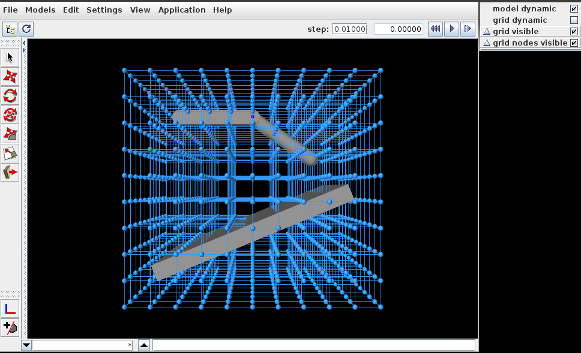
\includegraphics[]{images/DeformedJointedCollide}
\else
 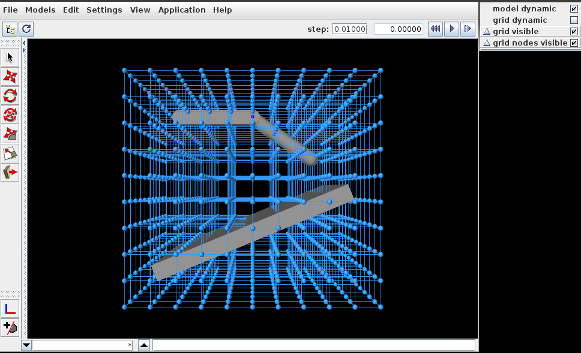
\includegraphics[width=5in]{images/DeformedJointedCollide}
\fi
\end{center}
\caption{The DeformedJointedCollide example initially loaded
into ArtiSynth.}
\label{DeformedJointedCollide:fig}
\end{figure}

To load this example in ArtiSynth, select {\sf All demos > tutorial >
DeformedJointedCollide} from the {\sf Models} menu. The model should load and
initially appear as in Figure \ref{DeformedJointedCollide:fig}, where
the control panel appears on the right.

The underlying {\tt MechModel} (or "model") can now be
transformed by first deforming the FEM model (or "grid") and
then using the resulting deformation field to effect the
transformation:

\begin{enumerate}

\item Make the model non-dynamic and the grid dynamic by unchecking
{\sf model dynamic} and checking {\sf grid dynamic} in the control
panel. This means that when simulation is run, the model will be inert
while the grid will respond physically.

\item Deform the grid using simulation. One easy way to do this is to
fix certain nodes, generally on or near the grid boundary, and then
move some of these using the translation or transrotator
tool while simulation is running. To fix a set of nodes, select
them in the viewer, choose {\sf Edit properties ...} from the
right-click context menu, and then uncheck their {\sf dynamic} property.
To easily select a large number of nodes without also selecting
model components or grid elements, one can specify {\tt FemNode}
in the selection filter widget. (See the sections
``Manipulation Tools'' and ``Selection filering'' in the
\href{../uiguide/uiguide.html}{ArtiSynth User Interface Guide}.)

\item After the grid has been deformed, choose {\sf deform} from the
{\sf Application} menu in the ArtiSynth toolbar to transform the model.
Afterwards, the transformation can be undone by choosing {\sf undo},
and the grid can be reset by choosing {\sf reset grid}.

\item To run the deformed model after the transformation, it should
again be made dynamic by checking {\sf model dynamic} in the control
panel.  The itself grid can be made non-dynamic, and it and/or its
nodes can be made invisible by unchecking {\sf grid visible} and/or
{\sf grid nodes visible} in the control panel.

\end{enumerate}

The result of a possible deformation is shown in Figure
\ref{JointedCollideDeformation:fig}.

\begin{figure}[ht]
\begin{center}
  \begin{tabular}{cc}
  \iflatexml
    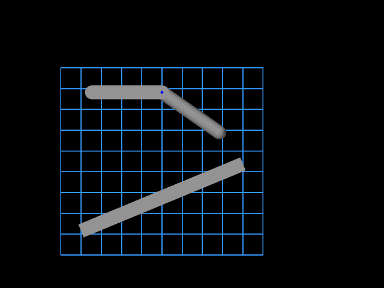
\includegraphics[]{images/DeformedJointedCollideBefore}&
    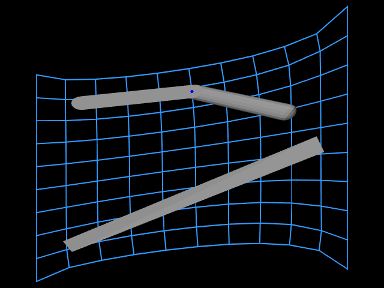
\includegraphics[]{images/DeformedJointedCollideAfter}
  \else
    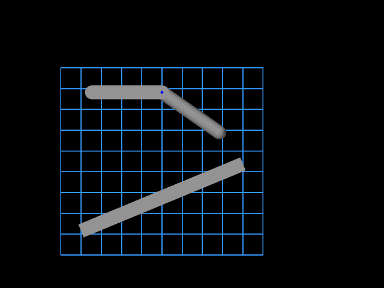
\includegraphics[width=0.45\textwidth]{images/DeformedJointedCollideBefore}&
    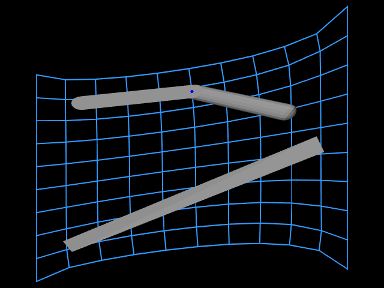
\includegraphics[width=0.45\textwidth]{images/DeformedJointedCollideAfter}
  \fi
  \end{tabular}
\end{center}
\caption{Deformation achieved in DeformedJointedCollide,
showing both the model and grid (using an orthographic view)
before and after the deformation.}
\label{JointedCollideDeformation:fig}
\end{figure}

\begin{sideblock}
Note: {\tt FemModelDeformer} is not intended to provide a general
purpose solution to non-linear geometric transformations. Rather, it
is mainly intended to illustrate the capabilities of
\javaclass[maspack.geometry]{GeometryTransformer} and the
\javaclass[artisynth.core.modelbase]{TransformableGeometry} interface.
\end{sideblock}

\subsubsection{Implementation and behavior}

As indicated above, the management of transforming the geometry for one
or more components is handled by the
\javaclass[artisynth.core.modelbase]{TransformGeometryContext} class.
The transform operations themselves are carried out by this class's
\javamethod[artisynth.core.modelbase.TransformGeometryContext]{apply()} 
method, which (a) assembles all the components that need
to be transformed, (b) performs the actual transform operations,
(c) invokes any required updating actions on other components,
and finally (d) notifies parent components of the change using
a \javaclass[artisynth.core.modelbase]{GeometryChangeEvent}.

To support this, ArtiSynth components which implement
\javaclass[artisynth.core.modelbase]{TransformableGeometry}
must also supply the methods
%
\begin{lstlisting}[]
   public void addTransformableDependencies (
      TransformGeometryContext context, int flags);

   public void transformGeometry (
      GeometryTransformer gtr, TransformGeometryContext context, int flags);
\end{lstlisting}
%
The first method,
\javamethodAlt{%
artisynth.core.modelbase.TransformableGeometry.addTransformableDependencies()}%
{addTransformableDependencies(context,flags)}, 
is called in step (a) to add to the context any additional components
which should be transformed along with this component. This includes
any descendants which should be transformed, since the
transformation of these should not generally be done within {\tt
transformGeometry(gtr,context,flags)}.

The second method, 
\javamethodAlt{%
artisynth.core.modelbase.TransformableGeometry.transformGeometry(,,)}%
{transformGeometry(gtr,context,flags)}, is
called in step (b) to perform the actual transformation on this
component.  It should use the supplied geometry transformer {\tt gtr}
to transform its attributes, as well as {\tt context} to query what
other components are also being transformed and to request
any needed updating actions to be called in step (c).  The {\tt flags} argument
specifies conditions associated with the transformation, which at the
moment may currently include:

\begin{description}

\item[TG\_SIMULATING]\mbox{}

The system is currently simulating, and therefore it may not be
desirable to transform all attributes;

\item[TG\_ARTICULATED]\mbox{}

Rigid body articulation constraints should
be enforced as the transform proceeds.

\end{description}

Full details for all this are given in the documentation for
\javaclass[artisynth.core.modelbase]{TransformGeometryContext}.

The transforming behavior of a component is up to its implementing
method, but the following rules are generally observed:

\begin{enumerate}

\item Transformable descendents are also transformed, by using {\tt
addTransformableDependencies()} to add them to the context as described
above;

\item When the nodes of an FEM model (Section \ref{FEMModels:sec}) are
transformed, the rest positions are also transformed if the system is
not simulating (i.e., if the {\tt TG\_SIMULATING} flag is not set).
This also causes the mass of the adjacent nodes to be recomputed from
the densities of the adjacent elements;

\item When dynamic components are transformed, any attachments and
constraints associated with them are updated appropriately, but only
if the system is not simulating. Non-transforming dynamic components
that are attached to transforming components as slaves are generally
updated so as to follow the transforming components to which they are
attached.

\end{enumerate}

\subsubsection{Use in model registration}

Transforming model geometry can obviously be used as part of the
process of creating subject-specific biomechanical and anatomical
models. However, registration will generally require more that
geometric transformation, since other properties, such as material
stiffnesses, densities, and maximum forces will generally need to be
adjusted as well. As a specific example, when applying a geometric
transform to a model containing {\tt AxialSprings}, the {\tt
restLength} properties of the springs will be unchanged, whereas the
intial lengths may be, resulting in a different applied forces and
physical behaviour.

\subsection{General component arrangements}

As discussed in Section \ref{MechModel:sec} and elsewhere, a {\tt
MechModel} provides a number of predefined child components for
storing particles, rigid bodies, springs, constraints, and other
components.  However, applications are not required to store their
components in these containers, and may instead create any sort of
component arrangement desired.

For example, suppose that one wishes to create a biomechanical model
of both the right and left human arms, consisting of bones,
point-to-point muscles, and joints. The standard containers supplied
by \javaclass[artisynth.core.mechmodels]{MechModel} would require that
all the components be placed within the following containers:
%
\begin{lstlisting}[]
   rigidBodies          // all bones
   axialSprings         // all point-to-point muscles
   connectors           // all joints
\end{lstlisting}
%
Instead of this, one may wish to set up a more appropriate component
hierarchy, such as
%
\begin{lstlisting}[]
   leftArm              // left-arm components
      bones             //   left bones
      muscles           //   left muscles
      joints            //   left joints
   rightArm             // right-arm components
      bones             //   right bones
      muscles           //   right muscles
      joints            //   right joints
\end{lstlisting}
%
To do this, the application {\tt build()} method can create the
necessary hierarchy and then
populate it with whatever components are desired.  Before simulation
begins (or whenever the model structure is changed), the {\tt
MechModel} will recursively traverse the component hierarchy and
update whatever internal structures are needed to run the
simulation.

\subsubsection{Container components}

The generic class \javaclass[artisynth.core.modelbase]{ComponentList}
can be used as a container for model components of a specific type.
It can be created using a declaration of the form
%
\begin{lstlisting}
   ComponentList<Particle> list = new ComponentList<Type> (Type.class, name);
\end{lstlisting}
%
where {\tt Type} is the class type of the components and {\tt name} is
the name for the container. Once the container is created, it should
be added to the {\tt MechModel} (or another internal container) and 
populated with child components of the specified type.
For example,
\begin{lstlisting}[]
   MechModel mech; 
   ...
   ComponentList<Particle> parts = 
      new ComponentList<Particle> (Particle.class, "parts");
   ComponentList<Frame> frames = 
      new ComponentList<Frame> (Frame.class, "frames");

   // add containers to the mech model
   mech.add (parts); 
   mech.add (frames);
\end{lstlisting}
creates two containers named {\tt "parts"} and {\tt "frames"} for
storing components of type {\tt Particle} and {\tt Frame},
respectively, and adds them to a {\tt MechModel} referenced by {\tt
mech}.

In addition to {\tt ComponentList}, applications may use several
"specialty" container types which are subclasses of {\tt
ComponentList}:

\begin{description}

\item[RenderableComponentList]\mbox{}

A subclass of {\tt ComponentList}, that
has its {\it own} set of render properties which can be inherited by
its children. This can be useful for compartmentalizing render
behavior.  Note that it is {\it not} necessary to store renderable
components in a {\tt RenderableComponentList}; components stored in a
{\tt ComponentList} will be rendered too.

\item[PointList]\mbox{}

A {\tt RenderableComponentList} that is optimized for
rendering points, and also contains its own {\tt pointDamping}
property that can be inherited by its children.

\item[PointSpringList]\mbox{}

A {\tt RenderableComponentList} designed for
storing point-based springs. It contains a {\tt material} property that
specifies a default axial material that can be used by its children.

\item[AxialSpringList]\mbox{}

A {\tt PointSpringList} that is optimized for
rendering two-point axial springs.

\end{description}

If necessary, it is relatively easy to define one's own customined
list by subclassing one of the other list types. One of the main
reasons for doing so, as suggested above, is to supply default
properties to be inherited by the list's descendents.  

A component list which declares {\tt ModelComponent} as its type can
be used to store {\tt any} type of component, including other
component lists. This allows the creation of arbitrary component
hierarchies. Generally either\\
{\tt ComponentList<ModelComponent>} or 
{\tt RenderableComponentList<ModelComponent>} are
best suited to implement hierarchical groupings.

\subsubsection{Example: a net formed from balls and springs}

A simple example showing an arrangement of balls and springs formed into
a net is defined in
%
\begin{verbatim}
  artisynth.demos.tutorial.NetDemo
\end{verbatim}
%

\begin{figure}[ht]
\begin{center}
\iflatexml
 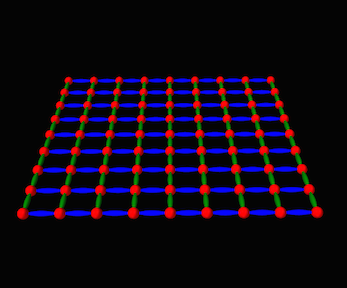
\includegraphics[]{images/NetDemo}
\else
 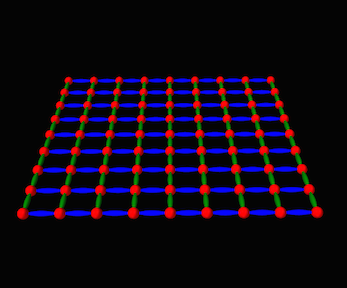
\includegraphics[width=3.75in]{images/NetDemo}
\fi
\end{center}
\caption{NetDemo model loaded into ArtiSynth.}
\label{NetDemo:fig}
\end{figure}

The {\tt build()} method and some of the supporting definitions for
this example are shown below.
%
\lstset{numbers=left}
\begin{lstlisting}[]
   protected double stiffness = 1000.0;   // spring stiffness
   protected double damping = 10.0;       // spring damping
   protected double maxForce = 5000.0;    // max force with excitation = 1
   protected double mass = 1.0;           // mass of each ball
   protected double widthx = 20.0;        // width of the net along x
   protected double widthy = 20.0;        // width of the net along y
   protected int numx = 8;                // num balls along x
   protected int numy = 8;                // num balls along y

   // custom component containers
   protected MechModel mech;
   protected PointList<Particle> balls;
   protected ComponentList<ModelComponent> springs;   
   protected RenderableComponentList<AxialSpring> greenSprings;
   protected RenderableComponentList<AxialSpring> blueSprings;

   private AxialSpring createSpring (
      PointList<Particle> parts, int idx0, int idx1) {
      // create a "muscle" spring connecting particles indexed by 'idx0' and
      // 'idx1' in the list 'parts'
      Muscle spr = new Muscle (parts.get(idx0), parts.get(idx1));
      spr.setMaterial (new SimpleAxialMuscle (stiffness, damping, maxForce));
      return spr;
   }

   public void build (String[] args) {

      // create MechModel and add to RootModel
      mech = new MechModel ("mech");
      mech.setGravity (0, 0, -980.0);
      mech.setPointDamping (1.0);
      addModel (mech);

      int nump = (numx+1)*(numy+1); // nump = total number of balls

      // create custom containers:
      balls = new PointList<Particle> (Particle.class, "balls");
      springs = new ComponentList<ModelComponent>(ModelComponent.class,"springs");
      greenSprings = new RenderableComponentList<AxialSpring> (
         AxialSpring.class, "greenSprings");
      blueSprings = new RenderableComponentList<AxialSpring> (
         AxialSpring.class, "blueSprings");

      // create balls in a grid pattern and add to the list 'balls'
      for (int i=0; i<=numx; i++) {
         for (int j=0; j<=numy; j++) {
            double x = widthx*(-0.5+i/(double)numx);
            double y = widthy*(-0.5+j/(double)numy);
            Particle p = new Particle (mass, x, y, /*z=*/0);
            balls.add (p);
            // fix balls along the edges parallel to y
            if (i == 0 || i == numx) {
               p.setDynamic (false);
            }
         }
      }

      // connect balls by green springs parallel to y
      for (int i=0; i<=numx; i++) {
         for (int j=0; j<numy; j++) {
            greenSprings.add (
               createSpring (balls, i*(numy+1)+j, i*(numy+1)+j+1));
         }
      }
      // connect balls by blue springs parallel to x
      for (int j=0; j<=numy; j++) {
         for (int i=0; i<numx; i++) {
            blueSprings.add (
               createSpring (balls, i*(numy+1)+j, (i+1)*(numy+1)+j));
         }
      }

      // add containers to the mechModel
      springs.add (greenSprings);
      springs.add (blueSprings);
      mech.add (balls);
      mech.add (springs);

      // set render properties for the components      
      RenderProps.setLineColor (greenSprings, new Color(0f, 0.5f, 0f));
      RenderProps.setLineColor (blueSprings, Color.BLUE);
      RenderProps.setSphericalPoints (mech, widthx/50.0, Color.RED);
      RenderProps.setCylindricalLines (mech, widthx/100.0, Color.BLUE);
   }
\end{lstlisting}
\lstset{numbers=none}
%
The {\tt build()} method begins by creating a {\tt MechModel} in the
usual way (lines 29-30). It then creates a net composed of a set of
balls arranged as a uniform grid in the x-y plane, connected by a set
of green colored springs running parallel to the y axis and a set of
blue colored springs running parallel to the x axis. These are
arranged into a component hierarchy of the form
%
\begin{lstlisting}[]
   balls
   springs
      greenSprings
      blueSprings
\end{lstlisting}
%
using containers created at lines 37-42. The balls are then created
and added to {\tt balls} (lines 45-56), the springs are created and
added to {\tt greenSprings} and {\tt blueSprings} (lines 59-71), and
the containers are added to the {\tt MechModel} at lines 74-77.
The balls along the edges parallel to the y axis are fixed.
Render properties are set at lines 80-83, with the colors for {\tt
greenSprings} and {\tt blueSprings} being explicitly set to dark green
and blue.

\begin{sideblock}
{\tt MechModel}, along with other classes derived from {\tt
ModelBase}, enforces {\it reference containment}. That means that all
components referenced by components within a {\tt MechModel} must
themselves be contained within the {\tt MechModel}.  This condition is
checked whenever a component is added directly to a {\tt MechModel} or
one of its ancestors. This means that the components must be added to
the {\tt MechModel} in an order that ensures any referenced components are
already present. For example, in the {\tt NetDemo} example above, adding the
particle list {\it after} the spring list would generate an error.
\end{sideblock}

To run this example in ArtiSynth, select {\sf All demos > tutorial >
NetDemo} from the {\sf Models} menu. The model should load and
initially appear as in Figure \ref{NetDemo:fig}.  Running the model
will cause the net to fall and sway under gravity. When the ArtiSynth
navigation panel is opened and expanded, the component hierarchy will
appear as in Figure \ref{NetDemoNav:fig}. While the standard
{\tt MechModel} containers are still present, they are not displayed
by default because they are empty.

\begin{figure}[ht]
\begin{center}
\iflatexml
 \includegraphics[]{images/NetDemoNav}
\else
 \includegraphics[width=2.25in]{images/NetDemoNav}
\fi
\end{center}
\caption{NetDemo components displayed in the ArtiSynth navigation panel.}
\label{NetDemoNav:fig}
\end{figure}

\subsubsection{Adding containers to other models}

In addition to {\tt MechModel}, application-defined containers can be
added to any model that inherits from
\javaclass[artisynth.core.modelbase]{ModelBase}. This includes {\tt
RootModel} and {\tt FemModel}. However, at the present time,
components added to such containers won't do anything, other than be
rendered in the viewer if they are
\javaclass[maspack.render]{Renderable}.




\section{Simulation Control}
\label{SimulationControl:sec}

This section describes different devices which an application may use
to control the simulation. These include {\it control panels} to allow
for the interactive adjustment of properties, as well as {\it agents}
which are applied every time step. Agents include {\it controllers}
and {\it input probes} to supply and modify input parameters at the
beginning of each time step, and {\it monitors} and {\it output
probes} to observe and record simulation results at the end of each
time step.

\subsection{Control Panels}
\label{ControlPanels:sec}

A {\it control panel} is an editing panel that allows for the
interactive adjustment of component properties.

It is always possible to adjust component properties through the GUI
by selecting one or more components and then choosing {\sf Edit
properties ...} in the right-click context menu. However, it may be
tedious to repeatedly select the required components, and the
resulting panels present the user with {\it all} properties common to
the selection.  A control panel allows an application to provide a
customized editing panel for selected properties.

\subsubsection{General principles}

Control panels are implemented by the
\javaclass[artisynth.core.gui]{ControlPanel} model component.  They
can be set up within a model's {\tt build()} method by creating an
instance of {\tt ControlPanel}, populating it with widgets for editing
the desired properties, and then adding it to the root model using the
latter's
\javamethod*[artisynth.core.workspace.RootModel]{addControlPanel()}
method.

One of the most commonly used means of adding widgets to a control
panel is the method
\javamethodAlt{artisynth.core.gui.ControlPanel.addWidget(HasProperties,String)}%
{addWidget(comp,propertyPath)}, which creates a widget for a property
specified by {\tt propertyPath} with respect to the component
{\tt comp}.  Property paths are discussed in the Section
\ref{PropertyHandlesAndPaths:sec}, and can consist solely of a
property name, or, for properties located in descendant components, a
component path followed by a colon '{\tt :}' and the property name.

Other flavors of {\tt addWidget()} also exist, as described in the API
documentation for \javaclass[artisynth.core.gui]{ControlPanel}.  In
addition to property widgets, any type of {\tt Swing} or {\tt awt}
component can be added using the method
\javamethodAlt{artisynth.core.gui.ControlPanel.addWidget(Component)}%
{addWidget(awtcomp)}.

Control panels can also be created interactively using the GUI; see
the section "Control Panels" in the
\href{../uiguide/uiguide.html}{
ArtiSynth User Interface Guide}.

\subsubsection{Example: Creating a simple control panel}

\begin{figure}[t]
\begin{center}
\iflatexml
 \includegraphics[]{images/controlPanel}
\else
 \includegraphics[width=3in]{images/controlPanel}
\fi
\end{center}
\caption{Control panel created by the model {\tt SimpleMuscleWithPanel}.}
\label{controlPanel:fig}
\end{figure}

An application model showing a control panel is defined in
%
\begin{verbatim}
  artisynth.demos.tutorial.SimpleMuscleWithPanel
\end{verbatim}
%
This model simply extends {\tt SimpleMuscle} (Section
\ref{SimpleMuscleExample:sec}) to provide a control panel for
adjusting gravity, the mass and color of the box, and the muscle
excitation. The class definition, excluding {\tt include} statements,
is shown below:
%
\lstset{numbers=left}
\begin{lstlisting}[]
public class SimpleMuscleWithPanel extends SimpleMuscle {
   ControlPanel panel;

   public void build (String[] args) throws IOException {

      super.build (args);

      // add control panel for gravity, rigod body mass and color, and excitation
      panel = new ControlPanel("controls");
      panel.addWidget (mech, "gravity");
      panel.addWidget (mech, "rigidBodies/box:mass");
      panel.addWidget (mech, "rigidBodies/box:renderProps.faceColor");
      panel.addWidget (new JSeparator());
      panel.addWidget (muscle, "excitation");

      addControlPanel (panel);
   }
}
\end{lstlisting}
\lstset{numbers=none}
%
The {\tt build()} method calls {\tt super.build()} to create the model
used by {\tt SimpleMuscle}. It then proceeds to create a {\tt
ControlPanel}, populate it with widgets, and add
it to the root model (lines 8-15). The panel is given the name {\tt
"controls"} in the constructor (line 8); this is its component name
and is also used as the title for the panel's window frame. A control
panel does not need to be named, but if it is, then that name must be
unique among the control panels.

Lines 9-11 create widgets for three properties located relative to the
{\tt MechModel} referenced by {\tt mech}. The first is the {\tt
MechModel}'s {\tt gravity}. The second is the {\tt mass} of the box,
which is a component located relative to {\tt mech} by the path name
(Section \ref{PathNames:sec}) {\tt "rigidBodies/box"}. The third is
the box's face color, which is the sub-property {\tt faceColor} of the
box's {\tt renderProps} property.

Line 12 adds a {\tt JSeparator} to the panel, using the {\tt
addWidget()} method that accepts general components, and line 13 adds
a widget to control the {\tt excitation} property for {\tt muscle}.

\begin{sideblock}
It should be noted that there are different ways to specify target
properties in {\tt addWidget()}. First, component paths may contain
numbers instead of names, and so the box's mass property could be
specified using {\tt "rigidBodies/0:mass"} instead of {\tt
"rigidBodies/box:mass"} since the box's number is 0. Second, if a
reference to a sub-component is available, one can specify properties
directly with respect to that, instead of indicating the sub-component
in the property path. For example, if the box was referenced by a
variable {\tt body}, then one could use the construction
%
\begin{verbatim}
   panel.addWidget (body, "mass");
\end{verbatim}
%
in place of 
%
\begin{verbatim}
   panel.addWidget (mech, "rigidBodies/box:mass");
\end{verbatim}
%
\end{sideblock}

To run this example in ArtiSynth, select {\sf All demos > tutorial >
SimpleMuscleWithPanel} from the {\sf Models} menu. The properties 
shown in the panel can be adjusted interactively by the user,
while the model is either stationary or running.
% SimpleMuscleWithPanel

\subsection{Custom properties}
\label{CustomProperties:sec}

Because of the usefulness of properties in creating control panels and
probes (Sections \ref{ControlPanels:sec}) and Section
\ref{Probes:sec}), model developers may wish to add their own
properties, either to the root model, or to a custom component.

This section provides only a brief summary of how to define
properties. Full details are available in the "Properties" section of
the \href{../maspack/maspack.html}{
Maspack Reference Manual}.

\subsubsection{Adding properties to a component}

As mentioned in Section \ref{Properties:sec}, properties are
class-specific, and are exported by a class through code contained in
the class's definition.  Often, it is convenient to add properties to
the {\tt RootModel} subclass that defines the application model. In
more advanced applications, developers may want to add properties to a
custom component.

The property definition steps are:

\begin{description}

\item[Declare the property list:]\mbox{}

The class exporting the properties creates its own static instance of
a \javaclass[maspack.properties]{PropertyList}, using a declaration
like
%
\begin{lstlisting}[]
   static PropertyList myProps = new PropertyList (MyClass.class, MyParent.class);

   @Override   
   public PropertyList getAllPropertyInfo() {
      return myProps;
   }  
\end{lstlisting}
%
where {\tt MyClass} and {\tt MyParent} specify the class types of the
exporting class and its parent class. The {\tt PropertyList}
declaration creates a new property list, with a copy of all the
properties contained in the parent class.  If one does {\it not} want
the parent class properties, or if the parent class does not have
properties, then one would use the constructor
\javamethodAlt{maspack.properties.PropertyList.PropertyList(Class)}%
{PropertyList(MyClass.class)} instead. If the parent class is an
ArtiSynth model component (including the {\tt RootModel}), then it
will always have its own properties. The declaration of the method
{\tt getAllPropertyInfo()} exposes the property list to other classes.

\item[Add properties to the list:]\mbox{}

Properties can then be added to the property list, by calling the {\tt
PropertyList}'s
\javamethod*[maspack.properties.PropertyList]{add(String,String,Object)}
method:
%
\begin{lstlisting}[]
   PropertyDesc add (String name, String description, Object defaultValue);
\end{lstlisting}
%
where {\tt name} contains the name of the property, {\tt description}
is a comment describing the property, and {\tt defaultValue} is an
object containing the property's default value.  This is done inside a
static code block:
%
\begin{lstlisting}[]
   static {
      myProps.add ("stiffness", "spring stiffness", /*defaultValue=*/1);
      myProps.add ("damping", "spring damping", /*defaultValue=*/0);
   }
\end{lstlisting}
%
Variations on the {\tt add()} method exist for adding {\it read-only}
or {\it inheritable} properties, or for setting various property
options. Other methods allow the property list to be edited.

\item[Declare property accessor functions:]\mbox{}

For each property {\tt propXXX} added to the property list, accessor methods of
the form
%
\begin{lstlisting}[]
   void setPropXXX (TypeX value) {
      ...
   }

   TypeX getPropXXX() {
      TypeX value = ...
      return value;
   }
\end{lstlisting}
%
must be declared, where {\tt TypeX} is the value associated with the
property. 
\begin{sideblock}
It is possible to specify different names for the accessor functions
in the string argument {\tt name} supplied to the {\tt add()}
method. Read-only properties only require a {\it get} accessor.
\end{sideblock}

\end{description}

\subsubsection{Example: a visibility property}
%
An model illustrating the exporting of properties is defined in
%
\begin{verbatim}
  artisynth.demos.tutorial.SimpleMuscleWithProperties
\end{verbatim}
%
This model extends {\tt SimpleMuscleWithPanel} (Section
\ref{SimpleMuscleExample:sec}) to provide a custom property
{\tt boxVisible} that is added to the control panel.
The class definition, excluding {\tt include} statements,
is shown below:
%
\lstset{numbers=left}
\begin{lstlisting}[]
public class SimpleMuscleWithProperties extends SimpleMuscleWithPanel {

   // internal property list; inherits properties from SimpleMuscleWithPanel
   static PropertyList myProps =
      new PropertyList (
         SimpleMuscleWithProperties.class, SimpleMuscleWithPanel.class);

   // override getAllPropertyInfo() to return property list for this class
   public PropertyList getAllPropertyInfo() {
      return myProps;
   }

   // add new properties to the list
   static {
      myProps.add ("boxVisible", "box is visible", false);
   }

   // declare property accessors
   public boolean getBoxVisible() {
      return box.getRenderProps().isVisible();
   }

   public void setBoxVisible (boolean visible) {
      RenderProps.setVisible (box, visible);
   }

   public void build (String[] args) throws IOException {

      super.build (args);

      panel.addWidget (this, "boxVisible");
      panel.pack();
   }
}
\end{lstlisting}
\lstset{numbers=none}
%
First, a property list is created for the application class {\tt
SimpleMuscleWithProperties.class} which contains a copy of all the
properties from the parent class {\tt SimpleMuscleWithPanel.class}
(lines 4-6). This property list is made visible by overriding {\tt
getAllPropertyInfo()} (lines 9-11). The {\tt boxVisible} property
itself is then added to the property list (line 15), and accessor
functions for it are declared (lines 19-25).

\begin{figure}[t]
\begin{center}
\iflatexml
 \includegraphics[]{images/boxVisiblePanel}
\else
 \includegraphics[width=3in]{images/boxVisiblePanel}
\fi
\end{center}
\caption{Control panel created by the model {\tt SimpleMuscleWithProperties},
showing the newly defined property {\tt boxVisible}.}
\label{boxVisiblePanel:fig}
\end{figure}

The {\tt build()} method calls {\tt super.build()} to perform all the
model creation required by the super class, and then adds an
additional widget for the {\tt boxVisible} property to the control
panel.

To run this example in ArtiSynth, select {\sf All demos > tutorial >
SimpleMuscleWithProperties} from the {\sf Models} menu. The control
panel will now contain an additional widget for the property {\tt
boxVisible} as shown in Figure \ref{boxVisiblePanel:fig}. Toggling
this property will make the box visible or invisible in the viewer.

% SimpleMuscleWithProperties

\subsection{Controllers and monitors}
\label{ControllersAndMonitors:sec}

Application models can define custom {\it controllers} and {\it
monitors} to control input values and monitor output values as a
simulation progresses. Controllers are called every time step
immediately before the {\tt advance()} method, and monitors are called
immediately after (Section \ref{ModelAdvancement:sec}).  An example of
controller usage is provided by ArtiSynth's inverse modeling feature,
which uses an internal controller to estimate the actuation signals
required to follow a specified motion trajectory.

More precise details about controllers and monitors and how they
interact with model advancement are given in the
\href{../artisynth/artisynth.html}{
ArtiSynth Reference Manual}.

\subsubsection{Implementation}
\label{ControllerImplementation:sec}

Applications may declare whatever controllers or monitors they require
and then add them to the root model using the methods
\javamethod*[artisynth.core.workspace.RootModel]{addController()} and
\javamethod*[artisynth.core.workspace.RootModel]{addMonitor()}.
They can be any type of
\javaclass[artisynth.core.modelbase]{ModelComponent} that implements
the \javaclass[artisynth.core.modelbase]{Controller} or
\javaclass[artisynth.core.modelbase]{Monitor} interfaces.  For
convenience, most applications simply subclass
\javaclass[artisynth.core.modelbase]{ControllerBase} or
\javaclass[artisynth.core.modelbase]{MonitorBase} and then override
the necessary methods.

The primary methods associated with both controllers and
monitors are:
%
\begin{lstlisting}[]
  public void initialize (double t0);

  public void apply (double t0, double t1);
\end{lstlisting}
%
{\tt apply(t0, t1)} is the "business" method and is called once per
time step, with {\tt t0} and {\tt t1} indicating the start and end
times $t_0$ and $t_1$ associated with the step.  {\tt initialize(t0)}
is called whenever an application model's state is set (or reset) at a
particular time $t_0$. This occurs when a simulation is first started
or after it is reset (with $t_0 = 0$), and also when the state is
reset at a waypoint or during adaptive stepping.

Controllers and monitors may be associated with a particular model
(among the list of models owned by the root model). This model may be
set or queried using
%
\begin{lstlisting}[]
  void setModel (Model m);

  Model getModel();
\end{lstlisting}
%
If associated with a model, {\tt apply()} will be called immediately
before (for controllers) or after (for monitors) the model's {\tt
advance()} method. If not associated with a model, then {\tt apply()}
will be called before or after the advance of {\it all} the models
owned by the root model.

Controllers and monitors may also contain {\it state}, in which case
they should implement the relevant methods from the
\javaclass[artisynth.core.modelbase]{HasState} interface.

Typical actions for a controller include setting input forces or
excitation values on components, or specifying the motion trajectory
of parametric components (Section \ref{DynamicVsParametric:sec}).
Typical actions for a monitor include observing or recording
the motion profiles or constraint forces that arise
from the simulation.

When setting the position and/or velocity of a dynamic component that
has been set to be parametric (Section \ref{DynamicVsParametric:sec}),
a controller should not set its position or velocity directly, but
should instead set its {\it target position} and/or {\it target
velocity}, since this allows the solver to properly interpolate the
position and velocity during the time step. The methods to set or
query target positions and velocities for
\javaclass[artisynth.core.modelbase]{Point}-based components are
%
\begin{lstlisting}[]
  setTargetPosition (Point3d pos);
  Point3d getTargetPosition ();       // read-only

  setTargetVelocity (Vector3d vel);
  Vector3d getTargetVelocity ();      // read-only
\end{lstlisting}
%
while for
\javaclass[artisynth.core.modelbase]{Frame}-based components they are
%
\begin{lstlisting}[]
  setTargetPosition (Point3d pos);
  setTargetOrientation (AxisAngle axisAng);
  setTargetPose (RigidTransform3d TFW);
  Point3d getTargetPosition ();       // read-only
  AxisAngle getTargetOrientation ();  // read-only
  RigidTransform3d getTargetPose();   // read-only

  setTargetVelocity (Twist vel);
  Twist getTargetVelocity ();         // read-only
\end{lstlisting}
%

\subsubsection{Example: A controller to move a point}

A model showing an application-defined controller is defined in
%
\begin{verbatim}
  artisynth.demos.tutorial.SimpleMuscleWithController
\end{verbatim}
%
This simply extends {\tt SimpleMuscle} (Section
\ref{SimpleMuscleExample:sec}) and adds a controller which moves the
fixed particle {\tt p1} along a circular path.  The complete class
definition is shown below:
%
\lstset{numbers=left}
\lstinputlisting{../../src/artisynth/demos/tutorial/SimpleMuscleWithController.java}
\lstset{numbers=none}
%
A controller called {\tt PointMover} is defined by extending {\tt
ControllerBase} and overriding the {\tt apply()} method. It stores the
point to be moved in {\tt myPnt}, and the initial position in
{\tt myPos0}. The {\tt apply()} method computes a target position for
the point that starts at {\tt myPos0} and then moves in a circle in the
$x-z$ plane with an angular velocity of $\pi/2$ rad/sec (lines 22-28).

The {\tt build()} method calls {\tt super.build()} to create the model
used by {\tt SimpleMuscle}, and then creates an instance of {\tt
PointMover} to move particle {\tt p1} and adds it to the root model
(line 34). The viewer bounds are updated to make the circular motion
more visible (line 36).

To run this example in ArtiSynth, select {\sf All demos > tutorial >
SimpleMuscleWithController} from the {\sf Models} menu. When
the model is run, the fixed particle {\tt p1} will trace
out a circular path in the $x-z$ plane.

\subsection{Probes}
\label{Probes:sec}

In addition to controllers and monitors, applications can also attach
streams of data, known as {\it probes}, to input and output values
associated with the simulation. Probes derive from the same base class
\javaclass[artisynth.core.modelbase]{ModelAgentBase} as 
controllers and monitors, 
but differ in that 

\begin{enumerate}

\item They are associated with an explicit time interval during which
they are applied;

\item They can have an attached file for supplying input data or
recording output data;

\item They are displayable in the ArtiSynth {\it timeline} panel.

\end{enumerate}

A probe is applied (by calling its {\tt apply()} method) only for time
steps that fall within its time interval. This interval can be set and
queried using the following methods:
%
\begin{lstlisting}[]
   setStartTime (double t0);
   setStopTime (double t1);
   setInterval (double t0, double t1);
 
   double getStartTime();
   double getStopTime();
\end{lstlisting}
%
The probe's attached file can be set and queried using:
%
\begin{lstlisting}[]
   setAttachedFileName (String fileName);
   String getAttachedFileName ();
\end{lstlisting}
%
where {\tt fileName} is a string giving the file's path name.

Details about the timeline display can be found in
the section "The Timeline" in the
\href{../uiguide/uiguide.html}{
ArtiSynth User Interface Guide}.

There are two types of probe: {\it input probes}, which are applied at
the beginning of each simulation step before the controllers, and {\it
output probes}, which are applied at the end of the step after the
monitors.

While applications are free to construct any type of probe by
subclassing either \javaclass[artisynth.core.probes]{InputProbe} or
\javaclass[artisynth.core.probes]{OutputProbe}, most applications
utilize either \javaclass[artisynth.core.probes]{NumericInputProbe} or
\javaclass[artisynth.core.probes]{NumericOutputProbe}, which
explicitly implement streams of numeric data which are connected to
properties of various model components.  The remainder of this section
will focus on numeric probes.

\subsubsection{Numeric probe structure}
\label{NumericProbeStructure:sec}

Numeric probes are associated with:

\begin{itemize}

\item {\it A vector of temporally-interpolated numeric data};

\item {\it One or more properties} to which the probe is bound and
which are either set by the numeric data (input probes), or used to
set the numeric data (output probes).

\end{itemize}

The numeric data is implemented internally by a
\javaclass[maspack.interpolation]{NumericList}, which stores the data
as a series of vector-valued knot points at prescribed times $t_k$ and
then interpolates the data for an arbitrary time $t$ using an
interpolation scheme provided by
\javaclass[maspack.interpolation]{Interpolation}.

Some of the numeric probe methods associated with the interpolated
data include:
%
\begin{lstlisting}[]
   int getVsize();                      // returns the size of the data vector
   setInterpolationOrder (Order order); // sets the interpolation scheme
   Order getInterpolationOrder();       // returns the interpolation scheme

   VectorNd getData (double t);         // interpolates data for time t
   NumericList getNumericList();        // returns the underlying NumericList
\end{lstlisting}
%
Interpolation schemes are described by the enumerated type {\tt
Interpolation.Order} and presently include:

\begin{description}

\item[Step]\mbox{}

Values at time $t$ are set to the values of the closest knot point
$k$ such that $t_k \le t$.

\item[Linear]\mbox{}

Values at time $t$ are set by linear interpolation of the knot points
$(k, k+1)$ such that $t_k \le t \le t_{k+1}$.

\item[Parabolic]\mbox{}

Values at time $t$ are set by quadratic interpolation of the knots
$(k-1, k, k+1)$ such that $t_k \le t \le t_{k+1}$.

\item[Cubic]\mbox{}

Values at time $t$ are set by cubic Catmull interpolation of the knots
$(k-1, \ldots, k+2)$ such that $t_k \le t \le t_{k+1}$.

\end{description}

Each property bound to a numeric probe must have a value
that can be mapped onto a scalar or vector value. Such properties
are know as {\it numeric properties}, and whether or not
a value is numeric can be tested
using \javamethodAlt{maspack.properties.NumericConverter.isNumeric()}%
{NumericConverter.isNumeric(value)}.

By default, the total number of scalar and vector values associated
with all the properties should equal the size of the interpolated
vector (as returned by
\javamethod*[artisynth.core.probes.NumericProbeBase]{getVsize()}).
However, it is possible to establish more complex mappings between the
property values and the interpolated vector. These mappings are beyond
the scope of this document, but are discussed in the sections "General
input probes" and "General output probes" of the
\href{../uiguide/uiguide.html}{
ArtiSynth User Interface Guide}.

\subsubsection{Creating probes in code}

This section discusses how to create numeric probes in code.  They can
also be created and added to a model graphically, as described in the
section "Adding and Editing Numeric Probes" in the
\href{../uiguide/uiguide.html}{
ArtiSynth User Interface Guide}.

Numeric probes have a number of constructors and methods that make it
relatively easy to create instances of them in code. For 
\javaclass[artisynth.core.probes]{NumericInputProbe}, there
is the constructor
%
\begin{lstlisting}[]
   NumericInputProbe (ModelComponent c, String propPath, String filePath);
\end{lstlisting}
%
which creates a {\tt NumericInputProbe}, binds it to a property
located relative to the component {\tt c} by {\tt propPath}, and then
attaches it to the file indicated by {\tt filePath} and loads data
from this file (see Section \ref{DataFileFormat:sec}). The probe's start and
stop times are specified in the file, and its vector size is
set to match the size of the scalar or vector value associated with
the property.

To create a probe attached to multiple properties, one may use the
constructor
%
\begin{lstlisting}[]
   NumericInputProbe (ModelComponent c, String propPaths[], String filePath);
\end{lstlisting}
%
which binds the probe to multiple properties specified relative to
{\tt c} by {\tt propPaths}. The probe's vector size is set to
the sum of the sizes of the scalar or vector values associated with
these properties.

For \javaclass[artisynth.core.probes]{NumericOutputProbe}, one may use
the constructor
%
\begin{lstlisting}[]
   NumericOutputProbe (ModelComponent c, String propPath, String filePath, double sample);
\end{lstlisting}
%
which creates a {\tt NumericOutputProbe}, binds it to the property
{\tt propPath} located relative to {\tt c}, and then attaches it to
the file indicated by {\tt filePath}. The argument {\tt sample}
indicates the {\it sample time} associated with the probe, in seconds;
a value of 0.01 means that data will be added to the probe every 0.01
seconds.  If {\tt sample} is specified as -1, then the sample time
will default to the maximum step size associated with the root model.

To create an output probe attached to multiple properties, one may use the
constructor
%
\begin{lstlisting}[]
   NumericOutputProbe (
      ModelComponent c, String propPaths[], String filePath, double sample);
\end{lstlisting}
%

\begin{sideblock}
As the simulation proceeds, an output probe will accumulate data, but
this data will not be saved to any attached file until the probe's
{\tt save()} method is called. This can be requested in the GUI for
all probes by clicking on the {\sf Save} button in the timeline
toolbar, or for specific probes by selecting them in the navigation
panel (or the timeline) and then choosing {\sf Save data} in the
right-click context menu.
\end{sideblock}

Output probes created with the above constructors have a default
interval of [0, 1]. A different interval may be set using
{\tt setInterval()}, {\tt setStartTime()}, or {\tt setStopTime()}.

\subsubsection{Example: probes connected to SimpleMuscle}
\label{SimpleMuscleWithProbes:sec}

A model showing a simple application of probes is defined in
%
\begin{verbatim}
  artisynth.demos.tutorial.SimpleMuscleWithProbes
\end{verbatim}
%
This extends {\tt SimpleMuscle} (Section
\ref{SimpleMuscleExample:sec}) to add an input probe to move particle
{\tt p1} along a defined path, along with an output probe to record
the velocity of the frame marker.  The complete class definition is
shown below:
%
\lstset{numbers=left}
\lstinputlisting{../../src/artisynth/demos/tutorial/SimpleMuscleWithProbes.java}
\lstset{numbers=none}
%
The input and output probes are added using the custom methods {\tt
createInputProbe()} and {\tt createOutputProbe()}. At line 14, {\tt
createInputProbe()} creates a new input probe bound to the {\tt
targetPosition} property for the component {\tt particles/p1} located
relative to the {\tt MechModel} {\tt mech}. The same constructor
attaches the probe to the file\\ {\tt simpleMuscleP1Pos.txt}, which is
read to load the probe data. The format of this and other probe data
files is described in Section \ref{DataFileFormat:sec}.  The method
\javamethod*[artisynth.core.util]{ArtisynthPath.getSrcRelativePath()}
is used to locate the file relative to the source directory for the
application model. The probe is then given the name {\tt "Particle
Position"} (line 18) and added to the root model (line 19).

Similarly, {\tt createOutputProbe()} creates a new output probe which
is bound to the {\tt velocity} property for the component {\tt
particles/0} located relative to {\tt mech}, is attached to the file {\tt
simpleMuscleMkrVel.txt} located in the application model source
directory, and is assigned a sample time of 0.01 seconds. This probe is
then named {\tt "FrameMarker Velocity"} and added to the root model.

The {\tt build()} method calls {\tt super.build()} to create
everything required for {\tt SimpleMuscle}, calls {\tt
createInputProbe()} and {\tt createOutputProbe()} to add the probes,
and adjusts the {\tt MechModel} viewer bounds to make the resulting
probe motion more visible.

To run this example in ArtiSynth, select {\sf All demos > tutorial >
SimpleMuscleWithProbes} from the {\sf Models} menu. After the model is
loaded, the input and output probes should appear on the timeline
(Figure \ref{probes:fig}). Expanding the probes should display their
numeric contents, with the knot points for the input probe clearly
visible.  Running the model will cause particle {\tt p1} to trace the
trajectory specified by the input probe, while the velocity of the
marker is recorded in the output probe. Figure
\ref{probesExpanded:fig} shows an expanded view of both probes after
the simulation has run for about six seconds.

% SimpleMuscleWithProbes

\begin{figure}[h]
\begin{center}
\iflatexml
 \includegraphics[]{images/timelineProbes}
\else
 \includegraphics[width=4in]{images/timelineProbes}
\fi
\end{center}
\caption{Timeline view of the probes created by SimpleMuscleWithProbes.}
\label{probes:fig}
\end{figure}

\begin{figure}[h]
\begin{center}
\iflatexml
 \includegraphics[]{images/timelineProbesExpanded}
\else
 \includegraphics[width=4in]{images/timelineProbesExpanded}
\fi
\end{center}
\caption{Expanded view of the probes after {\tt
SimpleMuscleWithProbes} has run for about 6 seconds, showing the data
accumulated in the output probe {\tt "FrameMarker Velocity"}.}
\label{probesExpanded:fig}
\end{figure}

\subsubsection{Data file format}
\label{DataFileFormat:sec}

The data files associated with numeric probes are ASCII files
containing two lines of header information followed by a set of knot
points, one per line, defining the numeric data. The time value
(relative to the probe's start time) for each knot point can be
specified explicitly at the start of the each line, in which case the
file takes the following format:
%
\begin{lstlisting}[]
startTime stopTime scale
interpolation vsize explicit
t0 val00 val01 val02 ...
t1 val10 val11 val12 ...
t0 val20 val21 val22 ...
...
\end{lstlisting}
%
Knot point information begins on line 3, with each line being a
sequence of numbers giving the knot's time followed by $n$ values,
where $n$ is the vector size of the probe (i.e., the value returned by
{\tt getVsize()}).

Alternatively, time values can be implicitly specified starting at 0
(relative to the probe's start time) and incrementing by a uniform
{\tt timeStep}, in which case the file assumes a second format:
%
\begin{lstlisting}[]
startTime stopTime scale
interpolation vsize timeStep
val00 val01 val02 ...
val10 val11 val12 ...
val20 val21 val22 ...
...
\end{lstlisting}
%
For both formats, {\tt startTime}, {\tt startTime}, and {\tt scale}
are numbers giving the probe's start and stop time in seconds and {\tt
scale} gives the scale factor (which is typically 1.0).  {\tt
interpolation} is a word describing how the data should be
interpolated between knot points and is the string value of {\tt
Interpolation.Order} as described in Section
\ref{NumericProbeStructure:sec} (and which is typically {\tt Linear},
{\tt Parabolic}, or {\tt Cubic}). {\tt vsize} is an integer giving the
probe's vector size.

The last entry on the second line is either a number specifying a
(uniform) time step for the knot points, in which case the file
assumes the second format, or the keyword {\tt explicit}, in which
case the file assumes the first format.

As an example, the file used to specify data for the input probe in
the example of Section \ref{SimpleMuscleWithProbes:sec} looks like
the following:
%
\begin{lstlisting}[]
0 4.0 1.0
Linear 3 explicit
0.0  0.0 0.0 0.0 
1.0  0.5 0.0 0.5
2.0  0.0 0.0 1.0
3.0 -0.5 0.0 0.5
4.0  0.0 0.0 0.0
\end{lstlisting}
%
Since the data is uniformly spaced beginning at 0, it would also be
possible to specify this using the second file format:
%
\begin{lstlisting}[]
0 4.0 1.0
Linear 3 1.0
 0.0 0.0 0.0 
 0.5 0.0 0.5
 0.0 0.0 1.0
-0.5 0.0 0.5
 0.0 0.0 0.0
\end{lstlisting}
%

\subsubsection{Adding probe data in-line}

It is also possible to specify input probe data directly in code,
instead of reading it from a file. For this, one would use the
constructor
%
\begin{lstlisting}[]
   NumericInputProbe (ModelComponent c, String propPath, double t0, double t1);
\end{lstlisting}
%
which creates a {\tt NumericInputProbe} with the specified property
and with start and stop times indicated by {\tt t0} and {\tt t1}.
Data can then be added to this probe using the method
%
\begin{lstlisting}[]
   addData (double[] data, double timeStep);
\end{lstlisting}
%
where {\tt data} is an array of knot point data. This contains the
same knot point information as provided by a file (Section
\ref{DataFileFormat:sec}), arranged in row-major order.  Times values
for the knots are either implicitly specified, starting at 0 (relative
to the probe's start time) and increasing uniformly by the amount
specified by {\tt timeStep}, or are explicitly specified at the
beginning of each knot if {\tt timeStep} is set to the built-in
constant {\tt NumericInputProbe.EXPLICIT\_TIME}. The size of the {\tt
data} array should then be either $n*m$ (implicit time values) or
$(n+1)*m$ (explicit time values), where $n$ is the probe's vector size
and $m$ is the number of knots.

As an example, the data for the input probe in Section
\ref{SimpleMuscleWithProbes:sec} could have been specified
using the following code:
%
\begin{lstlisting}[]
      NumericInputProbe p1probe =
         new NumericInputProbe (
            mech, "particles/p1:targetPosition", 0, 5);
      p1probe.addData (
         new double[] {
            0.0,  0.0, 0.0, 0.0,
            1.0,  0.5, 0.0, 0.5,
            2.0,  0.0, 0.0, 1.0,
            3.0, -0.5, 0.0, 0.5,
            4.0,  0.0, 0.0, 0.0 },
            NumericInputProbe.EXPLICIT_TIME);
\end{lstlisting}

When specifying data in code, the interpolation defaults to {\tt
Linear} unless explicitly specified using {\tt
setInterpolationOrder()}, as in, for example:
%
\begin{lstlisting}[]
   probe.setInterpolationOrder (Order.Cubic);
\end{lstlisting}
%
%


%!TEX root = modelguide.tex

% Scale latexml image sizes 2x
\newlength{\imglength}
\newcommand{\setlengthLaTeXML}[3]{ %
	\iflatexml %
	\setlength{#1}{#2} %
	\else %
	\setlength{#1}{#3} %
	\fi %
}

\section{Finite Element Models}
\label{FEMModels:sec}

This section details how to construct three-dimensional finite element models,
and how to couple them with the other simulation components described in
previous sections (e.g.~particles and rigid bodies).  Finite element
\emph{muscles}, which have additional properties that allow them to contract
given activation signals, are discussed in Section \ref{sec:fem:muscle}.  An 
example FEM model of the masseter, coupled to a rigid jaw and maxilla, is shown 
in Figure \ref{fig:fem:masseter}.

\begin{figure}[ht]
	\centering
	\setlengthLaTeXML{\imglength}{0.8\textwidth}{0.6\textwidth}
	\includegraphics[width=\imglength]{images/fem_masseter}
	\caption{Finite element model of the masseter, coupled to the jaw and 
	         maxilla. \label{fig:fem:masseter}} 
\end{figure}

\subsection{Overview}
\label{sec:fem:overview}

The finite element method (FEM) is a numerical technique used for solving a 
system of partial differential equations (PDEs) over some domain.  The general
approach is to divide the domain into a set of building blocks, referred to
as \emph{elements}.  These partition the space, and form local domains over
which the system of equations can be locally approximated. The corners of these
elements, the \emph{nodes}, become control points in a discretized system.  
The solution is then assumed to be
smoothly interpolated across the elements based on values determined at the
nodes.  Using this discretization, the differential system is converted into 
an algebraic one, which is often linearized and solved iteratively.

In ArtiSynth, the PDEs considered are the governing equations of
continuum mechanics: the conservation of mass, momentum, and energy.  To 
complete the system, a \emph{constitutive equation} is required that describes
the stress-strain response of the material.  This constitutive equation is what
distinguishes between material types.  The domain is the three-dimensional space
that the model occupies. This must be divided into small elements which 
accurately represent the geometry. Within each element, the PDEs are
sampled at a set of points, referred to as \emph{integration points}, and 
terms are numerically integrated to form an algebraic system to solve.

The purpose of the rest of this section is to describe the construction and
use of finite elements models within ArtiSynth.  It does not further discuss 
the mathematical framework or theory.
For an in-depth coverage of the nonlinear finite element method, as applied
to continuum mechanics, the reader is referred to the textbook by Bonet and 
Wood \cite{bonet:fem:2000}.

\subsubsection{FemModel3d}
\label{sec:fem:structure}

The basic type of finite element model is implemented in the class 
\javaclass[artisynth.core.femmodels]{FemModel3d}.  This class controls some
properties that are used by the model as a whole.  The key ones that affect
simulation dynamics are:
\begin{center}
	\begin{tabular}{|ll|}
		\hline
		Property & Description\\
		\hline
		{\tt density} & The density of the model\\
		{\tt material} & An object that describes the material's 
		    \emph{constitutive law} (i.e.~its stress-strain relationship).\\
		{\tt particleDamping} & Proportional damping associated with the 
		    particle-like motion of the FEM nodes.\\
		{\tt stiffnessDamping} & Proportional damping associated with the 
		    system's stiffness term.\\
		\hline
	\end{tabular}
\end{center}
These properties can be set and retrieved using the methods
\begin{lstlisting}[]
	setDensity ( double density );    // sets the density
	double getDensity ();             // gets the density

	setMaterial ( FemMaterial mat );  // sets the FEM's material
	FemMaterial getMaterial ();       // gets the FEM's material

	setParticleDamping ( double d );  // sets the particle (mass) damping coefficient
	double getParticleDamping ();     // gets the particle (mass) damping coefficient

	setStiffnessDamping ( double d ); // sets the stiffness damping coefficient
	double getStiffnessDamping ( );   // gets the stiffness damping coefficient
\end{lstlisting}
Keep in mind that ArtiSynth is essentially ``unitless'' (Section 
\ref{sec:mechii:units}), so it is the responsibility of the developer to
ensure that all properties are specified in a compatible way.  

The density of the model is used to compute the mass distribution throughout
the volume.  Note that we use a \emph{diagonally lumped mass matrix} (DLMM)
formulation, so the mass is assumed to be concentrated at the location of
the discretized FEM nodes.  To allow for a spatially-varying density,
a mass can later be specified for each node individually.

The FEM's {\tt material} is a delegate object used to compute stress and 
stiffness within individual elements.  It handles the \emph{constitutive}
component of the model.  Materials will be discussed in more detail in
Section \ref{sec:fem:materials}.

The two damping parameters are related to \emph{Rayleigh damping}, which
is used to dissipate energy within finite element models.  There are two 
proportional damping terms: one related to the system's mass, and one related 
to stiffness.  The resulting damping force applied is
\begin{align}
	\f_d & = - (d_M \M + d_K\K)\v,
\end{align}
where $d_M$ is the value of {\tt particleDamping}, $d_K$ is the value of 
{\tt stiffnessDamping}, $\M$ is the FEM model's lumped mass matrix, $\K$ is 
the FEM's stiffness matrix, and $\v$ is the concatenated vector of FEM node
velocities.  Since the lumped mass matrix is diagonal, the mass-related
component of damping can be applied separately to each FEM node.  Thus, the
mass component reduces to the same system as Equation \eqref{eqn:pointdamping},
which is why it is referred to as ``particle damping''.

\subsubsection{Component Structure}

Each \javaclass[artisynth.core.femmodels]{FemModel3d} contains three 
lists of sub-components:

\begin{description}
\item[{\tt nodes}]\mbox{}

The particle-like dynamic components of the model.  These lie at the corners
of the elements and carry all the mass (due to DLMM formulation).

\item[{\tt elements}]\mbox{}

The spatial building blocks of the model.  These define the sub-units over 
which the system is numerically integrated.

\item[{\tt meshes}]\mbox{}

The geometry in the model.  This includes the surface mesh, and any other
embedded geometries.
\end{description}

An example showing each of these components is shown in Figure \ref{fig:fem}.

\begin{figure}[ht]
	\centering
	%\subfigure[][FEM model \label{fig:fem:model}] {\includegraphics[width=0.2\textwidth]{images/fem_embedded.png}}
	%\subfigure[][Nodes \label{fig:fem:nodes}] {\includegraphics[width=0.2\textwidth]{images/fem_embedded_nodes.png}}
	%\subfigure[][Elements \label{fig:fem:elements}] {\includegraphics[width=0.2\textwidth]{images/fem_embedded_elements.png}}
	%\subfigure[][Geometry \label{fig:fem:geometry}] {\includegraphics[width=0.2\textwidth]{images/fem_embedded_geometry.png}}
	\setlengthLaTeXML{\imglength}{1.5in}{1.2in}
	\begin{tabular}{cccc}
	\includegraphics[width=\imglength]{images/fem_embedded.png} & 
	\includegraphics[width=\imglength]{images/fem_embedded_nodes.png} &
	\includegraphics[width=\imglength]{images/fem_embedded_elements.png} &
	\includegraphics[width=\imglength]{images/fem_embedded_geometry.png}\\
	(a) FEM model & (b) Nodes & (c) Elements & (d) Geometry
	\end{tabular}
	\caption{Sub-components of \javaclass[artisynth.core.femmodels]{FemModel3d}. \label{fig:fem}}
\end{figure}

\paragraph{Nodes}
\ifLaTeXML{\newline}

The set of nodes belong to a finite element model can be obtained by the method
\begin{lstlisting}[]
PointList<FemNode3d> getNodes();  // returns list of FEM nodes
\end{lstlisting}
Nodes are implemented in the class 
\javaclass[artisynth.core.femmodels]{FemNode3d}, which is a subclass of 
\javaclass[artisynth.core.mechmodels]{Particle} (Section 
\ref{ParticlesAndSprings:sec}).  They are the main dynamic components of
the finite element model.  The key properties affecting simulation dynamics
are:
\begin{center}
	\begin{tabular}{|ll|}
		\hline
		Property & Description\\
		\hline
		{\tt restPosition} & The initial position of the node.\\
		{\tt position} & The current position of the node.\\
		{\tt velocity} & The current velocity of the node.\\
		{\tt mass} & The mass of the node.\\
		{\tt dynamic} & Whether the node is considered dynamic or parametric 
		                (e.g.~boundary condition).\\
		\hline
	\end{tabular}
\end{center}
Each of these properties has corresponding {\tt getXxx()} and 
{\tt setXxx(...)} functions to access and modify them.

The {\tt restPosition} property defines the node's position in the FEM model's 
``natural'' or ``undeformed'' state.  Rest positions are used to compute
an initial configuration for the model, from which strains are determined.  A
node's rest position can be updated in code using the method:
\javamethod[artisynth.core.femmodels]{FemNode3d.setRestPosition(Point3d)}.

\begin{sideblock}
If any node's rest positions are changed, the current values 
for stress and stiffness will become invalid.  They can be manually
updated using the method \javamethod[artisynth.core.femmodels] %
{FemModel3d.updateStressAndStiffness()} for the parent model. Otherwise,
stress and stiffness will be automatically updated at the beginning of the 
next time step. 
\end{sideblock}

The properties {\tt position} and {\tt velocity} give the node's current
3D state.  These are common to all point-like particles, as is the 
{\tt mass} property.  Here, however, {\tt mass} represents the lumped mass
of the immediately surrounding material.  Its value is initialized by equally
dividing mass contributions from each adjacent element, given their
densities.  For a finer control of spatially-varying density,
node masses can be set manually after FEM creation.

The FEM node's {\tt dynamic} property specifies whether or not the 
node is considered when computing the dynamics of the system.  If not,
it is treated as being parametrically controlled.  This has implications
when setting boundary conditions (Section \ref{sec:fem:boundary}).

\paragraph{Elements}
\ifLaTeXML{\newline}

Elements are the spatial building blocks of the domain.  Within each element,
the displacement (or strain) field is interpolated from displacements at nodes:
\begin{align}
	\u(\x) & = \sum_{i=1}^N \phi_i(\x)\u_i, \label{eqn:fem:interp}
\end{align}
where $\u_i$ is the displacement of the $i$th node that is adjacent to the 
element, and $\phi_i(\cdot)$ is referred to as the \emph{shape function} (or 
\emph{basis function}) associated with that node.  Elements are classified by 
their shape, number of nodes, and shape function order (Table 
\ref{tbl:fem:elements}).  ArtiSynth supports the following element types:
\begin{center}
	\setlengthLaTeXML{\imglength}{1.5in}{1in}
	\begin{tabular}{c@{\hspace{5ex}}c@{\hspace{5ex}}c@{\hspace{5ex}}c}
		\includegraphics[height=\imglength]{images/fem_element_tet} &
		\includegraphics[height=\imglength]{images/fem_element_pyramid} &
		\includegraphics[height=\imglength]{images/fem_element_wedge} &
		\includegraphics[height=\imglength]{images/fem_element_hex} \\
		\javaclass[artisynth.core.femmodels]{TetElement}, &
		\javaclass[artisynth.core.femmodels]{PyramidElement}, & 
		\javaclass[artisynth.core.femmodels]{WedgeElement}, &
		\javaclass[artisynth.core.femmodels]{HexElement},\\
		\javaclass[artisynth.core.femmodels]{QuadtetElement} &
		\javaclass[artisynth.core.femmodels]{QuadpyramidElement} & 
		\javaclass[artisynth.core.femmodels]{QuadwedgeElement} &
		\javaclass[artisynth.core.femmodels]{QuadhexElement}
	\end{tabular}
\end{center}
\begin{table}[ht]
\centering
\caption{Supported element types \label{tbl:fem:elements}}
\begin{tabular}{lccc}
	\hline\hline
	Element Type & \# Nodes & Order &  \# Integration Points \\
	\hline
	\javaclass[artisynth.core.femmodels]{TetElement} & 4 & linear & 1\\
	\javaclass[artisynth.core.femmodels]{PyramidElement} & 5 & linear & 5\\
	\javaclass[artisynth.core.femmodels]{WedgeElement} & 6 & linear & 6\\
	\javaclass[artisynth.core.femmodels]{HexElement} & 8 & linear & 8\\
	\javaclass[artisynth.core.femmodels]{QuadtetElement} & 10 & quadratic & 4\\
	\javaclass[artisynth.core.femmodels]{QuadpyramidElement} & 13 & quadratic & 5\\
	\javaclass[artisynth.core.femmodels]{QuadwedgeElement} & 15 & quadratic & 9\\
	\javaclass[artisynth.core.femmodels]{QuadhexElement} & 20 & quadratic & 14\\
	\hline
\end{tabular}
\end{table}
The base class for all of these is \javaclass[artisynth.core.femmodels]%
{FemElement3d}.  A numerical integration is performed within each element
to create the (tangent) stiffness matrix.  This integration is performed
by evaluating the stress and stiffness at a set of \emph{integration points}
within each element, and applying numerical quadrature.  The list of elements
in a model can be obtained with the method
\begin{lstlisting}[]
RenderableComponentList<FemElement3d> getElements();  // return the list of elements
\end{lstlisting}

All objects of type \javaclass[artisynth.core.femmodels]{FemModel3d} have the 
following properties:
\begin{center}
	\begin{tabular}{|ll|}
		\hline
		Property & Description\\
		\hline
		{\tt density} & Density of the element\\
		{\tt material} & An object that describes the \emph{constitutive law} 
		                 within the element (i.e.~its stress-strain 
		                 relationship).\\
		\hline
	\end{tabular}
\end{center}

If left unspecified, the element's {\tt density} is inherited from the 
containing {\tt FemModel3d} object.  When set, the mass of the element is
computed and divided amongst all its nodes, updating the lumped mass
matrix.

Each element's' {\tt material} property is also inherited by default from the 
containing {\tt FemModel3d}. Specifying a material here allows for spatially-%
varying material properties across the model.  Materials will be discussed
further in Section \ref{sec:fem:materials}.

\paragraph{Meshes}
\ifLaTeXML{\newline}

The geometry associated with a finite element model consists of a collection
of meshes (e.g.~\javaclass[maspack.geometry]{PolygonalMesh}, \javaclass[maspack.geometry]{PolylineMesh},
\javaclass[maspack.geometry]{PointMesh}) that move along with the
model in a way that maintains the shape function interpolation equation 
\eqref{eqn:fem:interp}
at each vertex location.  These geometries can be used for visualizations, or 
for physical interactions like collisions.  However, they have no physical 
properties themselves. FEM geometries will be discussed in more detail in 
Section \ref{sec:fem:geometry}.  The list of meshes can be obtained with the 
method
\begin{lstlisting}[]
MeshComponentList<FemMeshComp> getMeshComps();   // return the list of meshes in a FEM
\end{lstlisting}

\subsubsection{Materials}
\label{sec:fem:materials}

The stress-strain relationship within each element is defined by a ``material''
delegate object, implemented by a subclass of 
\javaclass[artisynth.core.materials]{FemMaterial}.  This material object is 
responsible for implementing the functions:
%
\begin{lstlisting}[]
   public void computeStress (...)  // computes the symmetric stress tensor
   public void computeTangent (...) // computes the local tangent stiffness matrix
\end{lstlisting}
%
Inputs include a deformation gradient, pressure, and a coordinate frame that
specifies potential directions of anisotropy. The default material type is 
\javaclass[artisynth.core.materials]{LinearMaterial}, where stress is related 
to strain through:
\begin{gather}
  \sigma(\x) = D\,\epsilon(\x), \label{eqn:fem:mat:linear}\\
  \text{where }\quad D = \begin{bmatrix}
	  \lambda +2\mu & \lambda & \lambda  & 0 & 0 & 0\\
	  \lambda &  \lambda +2\mu & \lambda & 0 & 0 & 0\\
	  \lambda & \lambda & \lambda +2\mu & 0 & 0 & 0\\
	  0 & 0 & 0 & \mu & 0 & 0\\
	  0 & 0 & 0 & 0 & \mu & 0\\
	  0 & 0 & 0 & 0 & 0 & \mu
        \end{bmatrix}, \quad \lambda = \dfrac{E\nu}{(1+\nu)(1-2\nu)},  \quad
      \mu = \dfrac{E}{2(1+\nu)},\notag
\end{gather}
$\sigma$ is the standard $6\times 1$ stress vector, $\epsilon$ is the 
strain vector, $E$ is the Young's Modulus, and $\nu$ is Poisson's ratio. This
linear material uses a corotational formulation, so rotations are removed
per element before computing the strain \cite{ngan:fem:2008}.  To enable or
disable this corotational formulation, use 
\javamethod[artisynth.core.materials]{LinearMaterial.setCorotated(boolean)}.

All material models, including linear and non-linear, are available in the package  
{\tt artisynth.core.materials}.  A list of common materials is provided in 
Table \ref{tbl:fem:materials}.  Those that are subclasses of 
\javaclass[artisynth.core.materials]{IncompressibleMaterial} allow for 
incompressibility.

\begin{table}[ht]
	\centering
 	\caption{Commonly used FEM materials \label{tbl:fem:materials}}
 	\begin{tabular}{|lll|}
 		\hline
 		\hline
 		Material & Parameters & \\
 		\hline
 		\javaclass[artisynth.core.materials]{LinearMaterial} & $E$ & Young's modulus \\
 		& $\nu$ & Poisson's ratio\\
 		& corotated & corotational formulation\\
 		\hline
 		\javaclass[artisynth.core.materials]{StVenantKirchoffMaterial} & $E$ & Young's modulus\\
 		& $\nu$ & Poisson's ratio\\
 		\hline
 		\javaclass[artisynth.core.materials]{NeoHookeanMaterial} & $E$ & Young's modulus\\
 		& $\nu$ & Poisson's ratio\\
 		\hline
 		\javaclass[artisynth.core.materials]{IncompressibleNeoHookeanMaterial} & $G$ & shear modulus\\
 		& $\kappa$ & bulk modulus\\
 		\hline
 		\javaclass[artisynth.core.materials]{MooneyRivlinMaterial} & $C_{10},C_{01},C_{20},C_{02}$ & distortional parameters\\
 		& $\kappa$ & bulk modulus\\
 		\hline
 		\javaclass[artisynth.core.materials]{OgdenMaterial} & $\mu_1,\ldots,\mu_6$ & material parameters\\
 		& $\alpha_1,\ldots,\alpha_6$ &\\
 		& $\kappa$ & bulk modulus\\
		\hline
	\end{tabular}
\end{table}


\subsubsection{Boundary conditions}
\label{sec:fem:boundary}

Boundary conditions can be implemented in one of several ways:
\begin{enumerate}
	\item Explicitly setting FEM node positions/velocities
	\item Attaching FEM nodes to other dynamic components
	\item Enabling collisions
\end{enumerate}
To enforce an explicit (Dirichlet) boundary condition for a set of  
nodes, their {\tt dynamic} property must be set to {\tt false}.  This notifies
ArtiSynth that the state of these nodes (both position and velocity) will 
be controlled parametrically.  By disabling dynamics, a fixed 
boundary condition is applied.  For a moving boundary, positions and velocities 
of the boundary nodes must be explicitly set every timestep.  This can be 
accomplished with either a \javaclass[artisynth.core.modelbase]{Controller} 
(see Section \ref{ControllersAndMonitors:sec}) or an 
\javaclass[artisynth.core.probes]{InputProbe} (see Section \ref{Probes:sec}).
Note that both the position \emph{and} velocity of the nodes should be
explicitly set for consistency.

Another type of supported boundary condition is to attach FEM nodes to other
components, including particles, springs, rigid bodies, and locations within
other FEM elements.  Here, the node is still considered dynamic, but its
motion is coupled to that of the attached component through a constraint
mechanism. Attachments will be discussed further in Section 
\ref{sec:fem:nodeattachments}.

Finally, the boundary of a FEM can be constrained by enabling collisions
with other components.  This will be covered in Section
\ref{sec:fem:collision}.


\subsection{FEM model creation}

Creating a finite element model in ArtiSynth typically follows the pattern:
\begin{lstlisting}[]
   // Create and add main MechModel
   MechModel mech = new MechModel("mech");
   addModel(mech);
      
   // Create FEM
   FemModel3d fem = new FemModel3d("fem");
   
   /* ... Setup FEM structure and properties ... */
   
   // Add FEM to model
   mech.addModel(fem); 
\end{lstlisting}
The main code block for the FEM setup should do the following:
\begin{itemize}
	\setlength{\itemsep}{-0.3em}
	\item Build the node/element structure
	\item Set physical properties%
	\ifLaTeXMLelse{}{\vspace{-0.5em}}
	\begin{itemize}
		\setlength{\itemsep}{-0.3em}
		\item density
		\item damping
		\item material
	\end{itemize} 
	\item Set boundary conditions
	\item Set render properties
\end{itemize}
Building the FEM structure can be done with the use of factory
methods for simple shapes, by loading external files, or by writing code
to manually assemble the nodes and elements.

\subsubsection{Factory methods}

For simple shapes such as beams and ellipsoids, there are factory methods to 
automatically build the node and element structure.  These methods are found
in the \javaclass[artisynth.core.femmodels]{FemFactory} class.  Some common
methods are
\begin{lstlisting}[]
FemFactory.createGrid(...)          // basic beam
FemFactory.createCylinder(...)      // cylinder
FemFactory.createTube(...)          // hollowed cylinder
FemFactory.createEllipsoid(...)     // ellipsoid
FemFactory.createTorus(...)         // torus
\end{lstlisting}
The inputs specify the dimensions, resolution, and potentially the type
of element to use.  The following code creates a basic beam made up of
hexahedral elements:
\begin{lstlisting}[]
// Create FEM
FemModel3d beam = new FemModel3d("beam");
      
// Build FEM structure
double[] size = {1.0, 0.25, 0.25};  // widths
int[] res = {8, 2, 2};              // resolution (# elements)
      
FemFactory.createGrid(beam, FemElementType.Hex,
	size[0], size[1], size[2], 
	res[0], res[1], res[2]);

/* ... Set FEM properties ... */

// Add FEM to model
mech.addModel(beam);
\end{lstlisting}

\subsubsection{Loading external FEM meshes}

For more complex geometries, volumetric meshes can be loaded from external
files.  A list of supported file types is provided in Table 
\ref{tbl:fem:fileformats}. To load a geometry, an appropriate file reader
must be created.  Readers capable of reading FEM models implement the 
interface \javaclass[artisynth.core.femmodels]{FemReader}, which has the
method
\begin{lstlisting}[]
readFem( FemModel3d fem )   // populates the FEM based on file contents
\end{lstlisting}
Additionally, many {\tt FemReader} classes have static methods to handle
the loading of files for convenience.

\begin{table}[ht]
	\centering
	\caption{Supported FEM geometry files \label{tbl:fem:fileformats}}
	\begin{tabular}{llll}
		\hline\hline
		Format & File extensions & Reader & Writer\\
		\hline
		ANSYS & .node, .elem & \javaclass[artisynth.core.femmodels]{AnsysReader} & \javaclass[artisynth.core.femmodels]{AnsysWriter}\\
		TetGen & .node, .ele & \javaclass[artisynth.core.femmodels]{TetGenReader} & \javaclass[artisynth.core.femmodels]{TetGenWriter}\\
		Abaqus & .inp & \javaclass[artisynth.core.femmodels]{AbaqusReader} & \javaclass[artisynth.core.femmodels]{AbaqusWriter}\\
		VTK (ASCII) & .vtk & \javaclass[artisynth.core.femmodels]{VtkAsciiReader} & \multicolumn{1}{c}{--}\\
		\hline
	\end{tabular}
\end{table}

The following code snippet demonstrates how to load a model using the
\javaclass[artisynth.core.femmodels]{AnsysReader}.
\begin{lstlisting}[]
// Create FEM
FemModel3d tongue = new FemModel3d("tongue");
      
// Read FEM from file
try {
   // Get files relative to THIS class
   String nodeFileName = ArtisynthPath.getSrcRelativePath(this, 
                            "data/tongue.node");
   String elemFileName = ArtisynthPath.getSrcRelativePath(this, 
                            "data/tongue.elem");

   AnsysReader.read(tongue, nodeFileName, elemFileName);

} catch (IOException ioe) {         
   // Wrap error, fail to create model
   throw new RuntimeException("Failed to read model", ioe);
}
      
// Add to model
mech.addModel(tongue);
\end{lstlisting}
The method \javamethod[artisynth.core.util]{ArtisynthPath.getSrcRelativePath()}
is used to find a path within the ArtiSynth source tree that is relative to the
current model's source file.  Note the try-catch block.  Most of these readers 
throw an {\tt IOException} if the read fails.

\subsubsection{Generating from surfaces}

There are two ways a FEM model can be generated from a surface: by using a
FEM mesh generator, and by extruding a surface along its normal direction.

ArtiSynth has the ability to interface directly with the TetGen library 
(\href{http://tetgen.org}{http://tetgen.org}) to create a tetrahedral 
volumetric mesh given a closed and manifold surface.  The main Java class for
calling TetGen directly is \javaclass[maspack.geometry]{TetgenTesselator}.
The tesselator has several advanced options, allowing for the computation of 
convex hulls, and for adding points to a volumetric mesh.  For simply creating
a FEM from a surface, there is a convenience routine within 
\javaclass[artisynth.core.femmodels]{FemFactory} that handles both mesh 
generation and constructing a {\tt FemModel3d}:
\begin{lstlisting}[]
// Create a FEM from a manifold mesh with a given quality
FemFactory.createFromMesh( PolygonalMesh mesh, double quality );
\end{lstlisting}
If {\tt quality} $>0$, then points will be added in an attempt to bound the
maximum radius-edge ratio (see the {\tt-q} switch for TetGen).  According
to the TetGen documentation, the algorithm \emph{usually} succeeds for a 
quality ratio of 1.2.

It's also possible to create thin layer of elements by extruding a surface
along its normal direction. 
\begin{lstlisting}[]
// Create a FEM by extruding a surface
FemFactory.createExtrusion(
      FemModel3d model, int nLayers, double layerThickness, double zOffset, 
      PolygonalMesh surface);
\end{lstlisting}
For example, to create a two-layer slice of elements centered about a 
surface of a tendon mesh, one might use
\begin{lstlisting}[]
// Load the tendon surface mesh
PolygonalMesh tendonSurface = new PolygonalMesh("tendon.obj");

// Create the tendon
FemModel3d tendon = new FemModel3d("tendon");
int layers = 2;             // 2 layers
double thickness = 0.0005;  // 0.5 mm layer thickness
double offset = thickness;  // center the layers about the surface

// Create the extrusion
FemFactory.createExtrusion( tendon, layers, thickness, offset, tendonSurface );
\end{lstlisting} 
For this type of extrusion, triangular faces become wedge elements, and 
quadrilateral faces become hexahedral elements.  

\begin{sideblock}
Note: for extrusions, no care is taken to ensure element quality; if the 
surface has a high curvature relative to the total extrusion thickness, 
then some elements will be inverted.
\end{sideblock}

\subsubsection{Building elements in code}

A finite element model's structure can also be manually constructed in code.  
\javaclass[artisynth.core.femmodels]{FemModel3d} has the methods:
\begin{lstlisting}[]
addNode ( FemNode3d );       // add a node to the model
addElement ( FemElement3d )  // add an element to the model
\end{lstlisting}
For an element to successfully be added, all its nodes must already have
been added to the model.  Nodes can be constructed from a 3D location, and
elements from an array of nodes.  A convenience routine is available in
\javaclass[artisynth.core.femmodels]{FemElement3d} that automatically creates
the appropriate element type given the number of nodes (Table 
\ref{tbl:fem:elements}):
\begin{lstlisting}[]
// Creates an element using the supplied nodes
FemElement3d FemElement3d.createElement( FemNode3d[] nodes );
\end{lstlisting}
Be aware of node orderings when supplying nodes.  For linear elements, 
ArtiSynth uses a clockwise convention with respect to the outward
normal for the first face, followed by the opposite node(s).  To determine the
correct ordering for a particular element, check the coordinates returned by 
the function 
\javamethod*[artisynth.core.femmodels]{FemElement3d.getNodeCoords()}.
This returns the concatenated coordinate list for an ``ideal'' element of
the given type.

\subsubsection{Example: a simple beam model}
\label{sec:fem:example:fembeam}

\begin{figure}[ht]
	\centering
	\setlengthLaTeXML{\imglength}{0.8\textwidth}{0.6\textwidth}
	\includegraphics[width=\imglength]{images/FemBeam}
	\caption{FemBeam model loaded into ArtiSynth.}
	\label{fig:fem:beam}
\end{figure}

A complete application model that implements a simple FEM beam is given below.
\lstset{numbers=left}
\lstinputlisting{../../src/artisynth/demos/tutorial/FemBeam.java}
\lstset{numbers=none}
This example can be found in {\tt artisynth.demos.tutorial.FemBeam}.  The 
{\tt build()} method first creates a {\tt MechModel} and {\tt FemModel3d}.
A FEM beam is created using a factory method on line 36.  This beam is
centered at the origin, so its length extends from {\tt-length/2} to 
{\tt length/2}.  The density, damping and material properties are then 
assigned.  

On lines 45--49, a fixed boundary condition is set to the left-hand side 
of the beam by setting the corresponding nodes to be non-dynamic.  Due to 
numerical precision, a small {\tt EPSILON} buffer is required to ensure 
all left-hand boundary nodes are identified (line 46).

Rendering properties are then assigned to the FEM model on line 52.  These 
will be discussed further in Section \ref{sec:fem:rendering}.

\subsection{FEM Geometry}
\label{sec:fem:geometry}

Associated with each FEM model is a list of geometry with the heading 
{\tt meshes}.  This geometry can be used for either display purposes, 
or for interactions such as collisions.  A geometry itself has no 
physical properties; its motion is entirely governed by the FEM model 
that contains it.  

All FEM geometries are of type \javaclass[artisynth.core.femmodels]{FemMeshComp}, 
which stores a reference to a mesh object (Section \ref{Meshes:sec}), as well
as attachment information that links vertices of the mesh to points within
the FEM.  The attachments enforce the shape function interpolation in Equation
\eqref{eqn:fem:interp} to hold at each mesh vertex, with constant shape function
coefficients.

\subsubsection{Surface meshes}

By default, every {\tt FemModel3d} has an auto-generated geometry representing
the ``surface mesh''.  The surface mesh consists of all un-shared element faces
(i.e.~the faces of individual elements that are exposed to the world), and its
vertices correspond to the nodes that make up those faces.  As the FEM nodes
move, so do the mesh vertices due to the attachment framework.

The surface mesh can be obtained using one of the following functions in 
{\tt FemModel3d}:
\begin{lstlisting}[]
FemMeshComp getSurfaceMeshComp ();     // returns the FemMeshComp surface component
PolygonalMesh getSurfaceMesh ();  // returns the underlying polygonal surface mesh
\end{lstlisting}
The first returns the surface complete with attachment information.  The latter 
method directly returns the {\tt PolygonalMesh} that is controlled by the FEM.  

It is possible to manually set the surface mesh:
\begin{lstlisting}[]
setSurfaceMesh ( PolygonalMesh surface );  // manually set surface mesh
\end{lstlisting}
However, doing so is normally not necessary.  It is always possible to add
additional mesh geometries to a finite element model, and the visibility
settings can be changed so that the default surface mesh is not rendered.  

\subsubsection{Embedding geometry within an FEM}

Any geometry of type \javaclass[maspack.geometry]{MeshBase} can be added to
a {\tt FemModel3d}.  To do so, first position the mesh so that its vertices 
are in the desired locations inside the FEM, then call one of the 
{\tt FemModel3d} methods:
\begin{lstlisting}[]
FemMeshComp addMesh ( MeshBase mesh );                // creates and returns FemMeshComp
FemMeshComp addMesh ( String name, MeshBase mesh );
\end{lstlisting}
The latter is a convenience routine that also gives the newly embedded
{\tt FemMeshComp} a name.

\subsubsection{Example: a beam with an embedded sphere}

\begin{figure}[ht]
	\centering
	\setlengthLaTeXML{\imglength}{0.8\textwidth}{0.6\textwidth}
	\includegraphics[width=\imglength]{images/FemEmbeddedSphere}
	\caption{FemEmbeddedSphere model loaded into ArtiSynth.}
	\label{fig:fem:embedded}
\end{figure}

A complete model demonstrating embedding a mesh is given below.
\lstset{numbers=left}
\lstinputlisting{../../src/artisynth/demos/tutorial/FemEmbeddedSphere.java}
\lstset{numbers=none}
This example can be found in {\tt artisynth.demos.tutorial.FemEmbeddedSphere}.
The model is very similar to {\tt FemBeam}.  A {\tt MechModel} and 
{\tt FemModel3d} are created and added.  At line 41, a {\tt PolygonalMesh}
of a sphere is created using a factory method.  The sphere is already
centered inside the beam, so it does not need to be repositioned.  At Line
42, the sphere is embedded inside model {\tt fem}, creating a {\tt FemMeshComp}
with the name ``sphere''.  The full model is shown in Figure 
\ref{fig:fem:embedded}.

\subsection{Node attachments}
\label{sec:fem:nodeattachments}

To couple FEM models to other dynamic components, the ``attachment''
mechanism described in Section \ref{PhysicsSimulation:sec} is used.
This involves creating and adding to the model attachment components,
which are instances of \javaclass[artisynth.core.mechmodels]{DynamicAttachment},
as described in Section \ref{Attachments:sec}.  
Common point-based
attachment classes are listed in Table \ref{tbl:fem:pointattachments}.

\begin{table}[ht]
	\centering
	\caption{Point-based attachments \label{tbl:fem:pointattachments}}

	\begin{tabular}{ll}
		\hline
		\hline
		Attachment & Description \\
		\hline
		\javaclass[artisynth.core.mechmodels]{PointParticleAttachment} & Attaches one ``point'' to one ``particle''\\
		\javaclass[artisynth.core.mechmodels]{PointFrameAttachment} & Attaches one ``point'' to one ``frame''\\
		\javaclass[artisynth.core.femmodels]{PointFem3dAttachment} &  Attaches one ``point'' to a linear combination of FEM nodes\\
		\hline
	\end{tabular}
\end{table}

FEM models are connected to other model components by attaching their
nodes to various components. This can be done by creating
an attachment object of the appropriate type, and then 
adding it to the {\tt MechModel} using
\begin{lstlisting}[]
  addAttachment (DynamicAttachment attach); // adds an attachment constraint
\end{lstlisting}
There are also convenience routines inside {\tt MechModel} that will create
the appropriate attachments automatically (see Section 
\ref{sec:mech:pointattachments}).

\subsubsection{Connecting nodes to rigid bodies or particles}

Since
\javaclass[artisynth.core.femmodels]{FemNode3d} is a subclass of
\javaclass[artisynth.core.mechmodels]{Particle}, the same methods
described in Section \ref{sec:mech:pointattachments} for attaching 
particles to other particles and frames are available. For example, 
we can attach an FEM node to a rigid body using a
either a statement of the form
%
\begin{lstlisting}[]
   mech.addAttachment (new PointFrameAttachment(body, node));
\end{lstlisting}
%
or the following equivalent statement which does the same thing:
%
\begin{lstlisting}[]
   mech.attachPoint (node, body);
\end{lstlisting}
%
Both of these create a {\tt PointFrameAttachment} between a rigid body (called
{\tt body}) and an FEM node (called {\tt node}) and then adds it to
the {\tt MechModel} {\tt mech}.

One can also attach the nodes of one FEM model to the nodes of another
using statements like
%
\begin{lstlisting}[]
   mech.addAttachment (new PointParticle (node1, node2));
\end{lstlisting}
%
or
%
\begin{lstlisting}[]
   mech.attachPoint (node2, node1);
\end{lstlisting}
%
which attaches {\tt node2} to {\tt node1}.

\subsubsection{Example: connecting a beam to a block}

\begin{figure}[ht]
	\centering
	\setlengthLaTeXML{\imglength}{0.8\textwidth}{0.6\textwidth}
	\includegraphics[width=\imglength]{images/FemBeamWithBlock}
	\caption{FemBeamWithBlock model loaded into artisynth.}
	\label{fig:fem:beamwithblock}
\end{figure}

The following model demonstrates attaching a FEM beam to a rigid block.
\lstset{numbers=left}
\lstinputlisting{../../src/artisynth/demos/tutorial/FemBeamWithBlock.java}
\lstset{numbers=none}
This model extends the {\tt FemBeam} example of Section 
\ref{sec:fem:example:fembeam}.  The {\tt build()} method then creates 
and adds a {\tt RigidBody} block (lines 18--20).  On line 21, the block
is repositioned to the side of the beam to prepare for the attachment.
On lines 24--28, all right-most nodes of the beam are then set to be attached
to the block using a {\tt PointFrameAttachment}.  In this case, the 
attachments are explicitly created.  They could also have been attached using
\begin{lstlisting}[]
   mech.attachPoint (node, block);  // attach node to rigid block
\end{lstlisting}

\subsubsection{Connecting nodes directly to elements}

Typically, nodes do not align in a way that makes it
possible to connect them to other FEM models and/or points based on
simple point-to-node attachments.  Instead, we use a different
mechanism that allows us to attach a point to an arbitrary location
within a FEM model. This is done using an attachment component of
type
\javaclass[artisynth.core.femmodels]{PointFem3dAttachment}, which
implements an attachment where the position $\p$ and velocity $\u$ of the
attached point is determined by a weighted sum of the positions $\p_k$ 
and velocities $\u_k$ of selected fem nodes:
%
\begin{equation}
\p = \sum w_k \p_k
\label{pointFemAttachment:eqn}
\end{equation}
%
Any force $\f$ acting on the attached point is then propagated back
to the nodes, according to the relation
%
\begin{equation}
\f_k = w_k \f
\label{pointFemForces:eqn}
\end{equation}
%
where $\f_k$ is the force acting on node $k$ due to $\f$.  This
relation can be derived based on the conservation of energy.
If $\p$ is embedded within a single element, then the $\p_k$ are
simply the element nodes and the $w_i$ are corresponding shape
function values; this is known as an {\it element-based} attachment.
On the other hand, as desribed below, it is sometimes desirable to
form an attachment using a more general set of nodes that extends
beyond a single element; this is known as a {\it nodal-based}
attachment (Section \ref{sec:fem:nodalAttachments}).

An element-based attachment can be created using a code fragment
of the form
%
\begin{lstlisting}[]
   PointFem3dAttachment ax = new PointFem3dAttachment(pnt);
   ax.setFromElement (pnt.getPosition(), elem);
   mech.addAttachment (ax);
\end{lstlisting}
%
First, a {\tt PointFem3dAttachment} is created for the point {\tt
pnt}. Next, {\tt setFromElement()} is used to determine the nodal
weights within the element {\tt elem} for the specified position
(which in this case is simply the point's current position).  To do
this, it computes the ``natural coordinates'' coordinates of the
position within the element. For this to be guaranteed to work, the
position should be on or inside the element. If natural coordinates
cannot be found, the method will return {\tt false} and the nearest
estimates coordinates will be used instead. However, it is
sometimes possible to find natural coordinates outside a given element
as long as the shape functions are well-defined. Finally, the
attachment is added to the model.

More conveniently, the exact same functionality is provided
by the {\tt attachPoint()} method in {\tt MechModel}:
%
\begin{lstlisting}[]
   mech.attachPoint (pnt, elem);
\end{lstlisting}
%
This creates an attachment identical to that created by the previous
code fragment.

Often, one does not want to have to determine the element 
to which a point should be attached. In that case, one can call
%
\begin{lstlisting}[]
   PointFem3dAttachment ax = new PointFem3dAttachment(pnt);
   ax.setFromFem (pnt.getPosition(), fem);
   mech.addAttachment (ax);
\end{lstlisting}
%
or, equivalently, 
%
\begin{lstlisting}[]
   mech.attachPoint (pnt, fem);
\end{lstlisting}
%
This will find the nearest element to the node in question and use
that to create the attachment. If the node is outside the FEM model,
then it will be attached to the nearest point on the FEM's surface.

\subsubsection{Example: connecting two FEMs together}
\label{connectingTwoFems:sec}

% FemBeamWithFemSphere
\begin{figure}[ht]
	\centering
	\setlengthLaTeXML{\imglength}{0.8\textwidth}{0.6\textwidth}
	\includegraphics[width=\imglength]{images/FemBeamWithFemSphere}
	\caption{FemBeamWithFemSphere model loaded into ArtiSynth.}
	\label{fig:fem:beamwithfemsphere}
\end{figure}

The following model demonstrates how to attach two FEM models together:
\lstset{numbers=left}
\lstinputlisting{../../src/artisynth/demos/tutorial/FemBeamWithFemSphere.java}
\lstset{numbers=none}
This example can be found in 
{\tt artisynth.demos.tutorial.FemBeamWithFemSphere}.  The model extends 
{\tt FemBeam}, adding a finite element sphere and coupling them together.
The sphere is created and added on lines 18--28.  It is read from
TetGen-generated files using the 
\javaclass[artisynth.core.femmodels]{TetGenReader} class.  The model is then
scaled to match the dimensions of the current model, and transformed to the
right side of the beam.  To create attachments, the code first checks for 
any nodes that belong to the sphere that fall inside the beam using the
\javamethod[artisynth.core.femmodels]{FemModel3d.findContainingElement(Point3d)}
method (line 36), which returns the containing element if the point is inside
the model, or {\tt null} if the point is outside.  Internally, this spatial 
search uses a bounding volume hierarchy for efficiency (see 
\javaclass[maspack.geometry]{BVTree} and 
\javaclass[maspack.geometry]{BVFeatureQuery}).  If the point is contained
within the beam, then {\tt mech.attachPoint()}
is used to attach it to the nodes of the element (line 39).

\subsubsection{Nodal-based attachments}
\label{sec:fem:nodalAttachments}

The example of Section \ref{connectingTwoFems:sec} uses element-based
attachments to connect the nodes of one FEM to elements of another.
As mentioned above, element-based attachments assume that the attached
point is associated with a specific FEM model element. 
While this often gives good results, there are situations where it may
be desirable to distribute the connection more broadly among a larger
set of nodes. 

In particular, this is sometimes the case when connecting FEM models
to point-to-point springs. The end-point of such a spring may end up
exerting a large force on the FEM, and then if the number of nodes to
which the end-point is attached are too small, the resulting forces on
these nodes (Equation \ref{pointFemForces:eqn}) may end up being too
large. In other words, it may be desirable to distribute the spring's
force more evenly throughout the FEM model. 

To handle such situations, it is possible to create a {\it
nodal-based} attachment in which the nodes and weights are explicitly
specified. This involves explicitly creating a {\tt
PointFem3dAttachment} for the point or particle to be attached and the
specifying the nodes and weights directly,
%
\begin{lstlisting}[]
   PointFem3dAttachment ax = new PointFem3dAttachment (part);
   ax.setFromNodes (nodes, weights);
   mech.addAttachment (ax);
\end{lstlisting}
%
where {\tt nodes} and {\tt weights} are arrays of {\tt FemNode} and
{\tt double}, respectively. It is up to the application to determine
these.

\javaclass[artisynth.core.femmodels]{PointFem3dAttachment} provides
several methods for explicitly specifying nodes and weights. The
signatures for these include:
\begin{lstlisting}[]
  void setFromNodes (FemNode[] nodes, double[] weights)
  void setFromNodes (Collection<FemNode> nodes, VectorNd weights)
  boolean setFromNodes (Point3d pos, FemNode[] nodes)
  boolean setFromNodes (Point3d pos, Collection<FemNode> nodes)
\end{lstlisting}
The last two methods determine the weights automatically, using an
inverse-distance-based calculation in which each weight $w_k$
is initially computed as
%
\begin{equation}
w_k = \frac{d_{\text{max}}}{d_k + d_{max}}
\label{invDistWeights:eqn}
\end{equation}
%
where $d_k$ is the distance from node $k$ to {\tt pos} and
$d_{\text{max}}$ is the maximum distance. The weights are then
adjusted to ensure that they sum to one and that the weighted sum of
the nodes equals {\tt pos}. In some cases, the specified nodes
may not provide enough support for the last condition to be
met, in which case the methods return {\tt false}.

\subsubsection{Example: element vs. nodal-based attachments}

\begin{figure}[ht]
\centering
\setlengthLaTeXML{\imglength}{0.8\textwidth}{0.6\textwidth}
\includegraphics[width=\imglength]{images/PointFemAttachment}
\caption{PointFemAttachment loaded into ArtiSynth and run until stable.
The top and bottom models are connected to their springs using element
and nodal-based attachments, respectively.  The nodes associated with
each attachment are rendered as white spheres.}
\label{fig:fem:pointFemAttachment}
\end{figure}

The model demonstrating the difference between element and
nodal-based attachments is defined in
%
\begin{verbatim}
  artisynth.demos.tutorial.PointFemAttachment
\end{verbatim}
%
It creates two FEM models, each
with a single point-to-point spring attached to a particle at their
center. The model at the top ({\tt fem1} in the code below) is
connected to the particle using an element-based attachment, while the
lower model ({\tt fem2} in the code) is connected using a nodal-based
attachment with a larger number of nodes. Figure
\ref{fig:fem:pointFemAttachment} shows the result after the model is
run until stable. The element-based attachment results in
significantly higher deformation in the immediate vicinity around the
attachment, while for the nodal-based attachment, the deformation is
distributed much more evenly through the model.

The build method and some of the auxiliary code for this model is shown below.
Code for the other auxiliary methods, including {\tt addFem()},
{\tt addParticle()}, {\tt addSpring()}, and {\tt setAttachedNodesWhite()},
can be found in the actual source file.
\lstset{numbers=left}
\begin{lstlisting}[]
   // Filter to select only elements for which the nodes are entirely on the
   // positive side of the x-z plane.
   private class MyFilter extends ElementFilter {
      public boolean elementIsValid (FemElement e) {
         for (FemNode n : e.getNodes()) {
            if (n.getPosition().y < 0) {
               return false;
            }
         }
         return true;         
      }
   }

   // Collect and return all the nodes of a FEM model associated with a
   // set of elements specified by an array of element numbers
   private HashSet<FemNode3d> collectNodes (FemModel3d fem, int[] elemNums) {
      HashSet<FemNode3d> nodes = new HashSet<FemNode3d>();
      for (int i=0; i<elemNums.length; i++) {
         FemElement3d e = fem.getElements().getByNumber (elemNums[i]);
         for (FemNode3d n : e.getNodes()) {
            nodes.add (n);
         }
      }
      return nodes;
   }

   public void build (String[] args) {
      MechModel mech = new MechModel ("mech");
      addModel (mech);
      mech.setGravity (0, 0, 0); // turn off gravity

      // create and add two FEM beam models centered at the specified locations
      FemModel3d fem1 = addFem (mech,  0.0, 0.0,  0.25);
      FemModel3d fem2 = addFem (mech,  0.0, 0.0, -0.25);

      // reconstruct the FEM surface meshes so that they show only elements on
      // the positive side of the x-y plane. Also, set surface rendering to
      // show strain values.
      fem1.createSurfaceMesh (new MyFilter());
      fem1.setSurfaceRendering (SurfaceRender.Strain);
      fem2.createSurfaceMesh (new MyFilter());
      fem2.setSurfaceRendering (SurfaceRender.Strain);

      // create and add the particles for the point-to-point springs
      // that will apply forces to each FEM.
      Particle p1 = addParticle (mech,  0.9, 0.0,  0.25);
      Particle p2 = addParticle (mech,  0.9, 0.0, -0.25);
      Particle m1 = addParticle (mech,  0.0, 0.0,  0.25);
      Particle m2 = addParticle (mech,  0.0, 0.0, -0.25);

      // attach spring end-point to fem1 using an element-based marker
      mech.attachPoint (m1, fem1);

      // attach spring end-point to fem2 using a larger number of nodes, formed
      // from the node set for elements 22, 31, 40, 49, and 58. This is done by
      // explicitly creating the attachment and then setting it to use the
      // specified nodes
      HashSet<FemNode3d> nodes =
         collectNodes (fem2, new int[] { 22, 31, 40, 49, 58 });

      PointFem3dAttachment ax = new PointFem3dAttachment (m2);
      ax.setFromNodes (m2.getPosition(), nodes);
      mech.addAttachment (ax);

      // finally, create the springs
      addSpring (mech, /*stiffness=*/10000, p1, m1);
      addSpring (mech, /*stiffness=*/10000, p2, m2);

      // set the attachments nodes for m1 and m2 to render as white spheres
      setAttachedNodesWhite (m1);
      setAttachedNodesWhite (m2);
      // set render properties for m1
      RenderProps.setSphericalPoints (m1, 0.015, Color.GREEN);
   }
\end{lstlisting}
\lstset{numbers=none}
The {\tt build()} method begins by creating a {\tt MechModel} and then
adding to it two FEM beams (created using the auxiliary method {\tt
addFem()}. Rendering of each FEM model's surface is then set up to
show strain values ({\tt setSurfaceRendering()}, lines 41 and 43).
The surface meshes themselves are also redefined to exclude the
frontmost elements, allowing the strain values to be displayed closer
model centers. This redefinition is done using calls to {\tt
createSurfaceMesh()} (lines 40, 41) with a custom {\tt ElementFilter}
defined at lines 3-12.

Next, the end-point particles for the axial springs are created (using
the auxiliary method {\tt addParticle()}, lines
46-49), and particle {\tt m1} is attached to {\tt fem1} using {\tt
mech.attachPoint()} (line 52), which creates an element-based
attachment at the point's current location. Point {\tt m2} is then
attached to {\tt fem2} using a nodal-based attachment.  The nodes for
these are collected as the union of all nodes for a specufied set of
elements (lines 58-59, and the method {\tt collectNodes()} defined at
lines 16-25). These are then used to create a nodal-based attachment
(lines 61-63), where the weights are determined automatically using
the method associated with equation (\ref{invDistWeights:eqn}).

Finally, the springs are created (auxiliary method {\tt addSpring()},
lines 66-67), the nodes associated for each attachment are set to
render as white spheres ({\tt setAttachedNodesWhites()}, lines 70-71),
and the particles are set to render as green spheres.

To run this example in ArtiSynth, select {\sf All demos > tutorial >
PointFemAttachment} from the {\sf Models} menu. Running the model will
cause it to settle into the state shown in Figure
\ref{fig:fem:pointFemAttachment}. Selecting and dragging one of the
spring anchor points at the right will cause the spring tension to
vary and further illustrate the difference between the element
and nodal-based attachments.

\subsection{FEM markers}

Just as there are {\tt FrameMarker}s to act as anchor points on a frame or
rigid body (Section \ref{FrameMarkers:sec}), there are also {\tt FemMarker}s 
that can mark a point inside a finite element.  They are frequently used to 
provide anchor points for attaching springs and forces to a point inside 
an element, but can also be used for graphical purposes.

FEM markers are implemented by the class
\javaclass[artisynth.core.femmodels]{FemMarker}, which
is a subclass of
\javaclass[artisynth.core.mechmodels]{Point}.
They are essentially massless points that contain their own attachment
component, so when creating and adding a marker there is no need to
create a separate attachment component.

Within the component hierarchy, FEM markers are typically stored in
the {\tt markers} list of their associated FEM model. They can
be created and added using a code fragment of the form
%
\begin{lstlisting}[]
  FemMarker mkr = new FemMarker (1, 0, 0);
  mkr.setFromFem (fem); // attach to the nearest fem element
  fem.addMarker (mkr);  // add to fem
\end{lstlisting}
%
This creates a marker at the location $(1,0,0)$ (in world
coordinates), calls {\tt setFromFem()} to attach it to the nearest
element in the FEM model ( which is either the containing element or
the nearest element on the model's surface), and then adds it to the
{\tt markers} list.

If the marker's attachment has not already been set when {\tt
addMarker()} is called, then {\tt addMarker()} will call {\tt
setFromFem()} automatically. Therefore the above code fragment is
equivalent to the following:
%
\begin{lstlisting}[]
  FemMarker mkr = new FemMarker (1, 0, 0);
  fem.addMarker (mkr);
\end{lstlisting}
%
Alternatively, one may want to explicitly specify the nodes
associated with the attachment, as described in Section 
\ref{sec:fem:nodalAttachments}:
%
\begin{lstlisting}[]
  FemMarker mkr = new FemMarker (1, 0, 0);
  mkr.setFromNodes (nodes, weights);
  fem.addMarker (mkr);
\end{lstlisting}
%
There are a variety of methods available to set the attachment, mirroring
those available in the underlying base class {\tt PointFem3dAttachment}:
\begin{lstlisting}[]
  void setFromFem (FemModel3d fem)
  boolean setFromElement (FemElement3d elem)
  void setFromNodes (FemNode[] nodes, double[] weights)
  void setFromNodes (Collection<FemNode> nodes, VectorNd weights)
  boolean setFromNodes (FemNode[] nodes)
  boolean setFromNodes (Collection<FemNode> nodes)
\end{lstlisting}
The last two methods compute nodal weights automatically, as described
in Section \ref{sec:fem:nodalAttachments}, based on the marker's
currently assigned position. If the supplied nodes do not provide
sufficient support, then the methods return {\tt false}.

Another set of convenience methods are supplied by {\tt FemModel3d},
which combine these with the {\tt addMarker()} call:
%
\begin{lstlisting}[]
  void addMarker (FemMarker mkr, FemElement3d elem)
  void addMarker (FemMarker mkr, FemNode[] nodes, double[] weights)
  void addMarker (FemMarker mkr, Collection<FemNode> nodes, VectorNd weights)
  boolean addMarker (FemMarker mkr, FemNode[] nodes)
  boolean addMarker (FemMarker mkr, Collection<FemNode> nodes)
\end{lstlisting}
%
For example, one can do
%
\begin{lstlisting}[]
  FemMarker mkr = new FemMarker (1, 0, 0);
  fem.addMarker (mkr, nodes, weights);
\end{lstlisting}
%

Markers are often used to track movement within an FEM model.
For that, one can examine their positions and velocities,
as with any other particles, using the methods
%
\begin{lstlisting}[]
  Point3d getPosition();     // returns the current position
  Vectord getVelocity();     // returns the current velocity
\end{lstlisting}
%
The return values from these methods should not be
modified. Alternatively, when a 3D force $\f$ is applied to the
marker, it is distributed to the attached nodes according to the nodel
weights, as described in Equation \eqref{pointFemForces:eqn}.

\subsubsection{Example: attaching a FEM beam to a muscle}

\begin{figure}[ht]
	\centering
	\setlengthLaTeXML{\imglength}{0.8\textwidth}{0.6\textwidth}
	\includegraphics[width=\imglength]{images/FemBeamWithMuscle}
	\caption{FemBeamWithMuscle model loaded into ArtiSynth.}
	\label{fig:fem:beamwithmuscle}
\end{figure}

A complete application model that employs a fem marker as an anchor for a spring
is given below.
\lstset{numbers=left}
\lstinputlisting{../../src/artisynth/demos/tutorial/FemBeamWithMuscle.java}
\lstset{numbers=none}
This example can be found in {\tt artisynth.demos.tutorial.FemBeamWithMuscle}.
This model extends the {\tt FemBeam} example, adding a {\tt FemMarker} for the
spring to attach to.  The method {\tt createMarker(...)} on lines 28--34
is used to create and add a marker to the FEM.  Since the element is initially
set to {\tt null}, when it is added to the FEM, the model searches for the
containing or nearest element.  The loaded model is shown in Figure 
\ref{fig:fem:beamwithmuscle}.

% FemBeamWithMuscle

\subsection{Frame attachments}
\label{sec:fem:frameattachments}

It is also possible to attach frame components, including rigid
bodies, directly to FEM models, using the attachment component
\javaclass[artisynth.core.femmodels]{FrameFem3dAttachment}.
Analagously to
\javaclass[artisynth.core.femmodels]{PointFem3dAttachment}, the
attachment is implemented by connecting the frame to a set of FEM
nodes, and attachments can be either element-based or nodal-based.  The
frame's origin is computed in the same way as for point attachments,
using a weighted sum of node positions (Equation
\ref{pointFemAttachment:eqn}), while the orientation is computed using
a polar decomposition on a deformation gradient determined from either
element shape functions (for element-based attachments) or a
Procrustes type analysis using nodal rest positions (for nodal-based attachments).

An element-based attachment can be created using either a code fragment
of the form
%
\begin{lstlisting}[]
   FrameFem3dAttachment ax = new FrameFem3dAttachment(frame);
   ax.setFromElement (frame.getPose(), elem);
   mech.addAttachment (ax);
\end{lstlisting}
%
or, equivalently, the {\tt attachFrame()} method in {\tt MechModel}:
%
\begin{lstlisting}[]
   mech.attachFrame (frame, elem);
\end{lstlisting}
%
This attaches the frame {\tt frame} to the nodes of the FEM element
{\tt elem}. As with {\tt PointFem3dAttachment}, if the frame's origin
is not inside the element, it may not be possible to accurately
compute the internal nodal weights, in which case {\tt
setFromElement()} will return {\tt false}.

In order to have the appropriate element located automatically,
one can instead use
%
\begin{lstlisting}[]
   FrameFem3dAttachment ax = new FrameFem3dAttachment(frame);
   ax.setFromFem (frame.getPose(), fem);
   mech.addAttachment (ax);
\end{lstlisting}
%
or, equivalently, 
%
\begin{lstlisting}[]
   mech.attachFrame (frame, fem);
\end{lstlisting}
%

As with point-to-FEM attachments, it may be desirable to create a
nodel-based attachment in which the nodes and weights are not tied to
a specific element. The reasons for this are generally the same as
with nodal-based point attachments (Section
\ref{sec:fem:nodalAttachments}): the need to distribute the forces and
moments acting on the frame across a broader set of element nodes.
Also, element-based frame attachments use element shape functions to
determine the frame's orientation, which may produce slightly
asymmetric results if the frame's origin is located particularly close
to a specific node.

\javaclass[artisynth.core.femmodels]{FrameFem3dAttachment} provides
several methods for explicitly specifying nodes and weights. The
signatures for these include:
\begin{lstlisting}[]
  void setFromNodes (RigidTransform3d TFW, FemNode[] nodes, double[] weights)
  void setFromNodes (RigidTransform3d TFW, Collection<FemNode> nodes, 
                        VectorNd weights)
  boolean setFromNodes (RigidTransform3d TFW, FemNode[] nodes)
  boolean setFromNodes (RigidTransform3d TFW, Collection<FemNode> nodes)
\end{lstlisting}
Unlike their counterparts in {\tt PointFem3dAttachment}, the first two
methods also require the current desired pose of the frame {\tt TFW}
(in world coordinates).  This is because while nodes and weights will
unambiguously specify the frame's origin, they do not specify the
desired orientation.

\subsubsection{Example: attaching frames to a FEM beam}

\begin{figure}[ht]
	\centering
	\setlengthLaTeXML{\imglength}{0.8\textwidth}{0.6\textwidth}
	\includegraphics[width=\imglength]{images/FrameFemAttachment}
	\caption{FrameFemAttachment loaded into ArtiSynth and run until stable.}
	\label{fig:fem:frameFemAttachment}
\end{figure}

A model illustrating how to connect frames to a FEM model 
is defined in
%
\begin{verbatim}
  artisynth.demos.tutorial.FrameFemAttachment
\end{verbatim}
%
It creates a FEM beam, along with a rigid body block and a 
massless coordinate frame, that are then attached to the beam
using nodal and element-based attachments. The build method is shown below:
\lstset{numbers=left}
\begin{lstlisting}[]
   public void build (String[] args) {

      MechModel mech = new MechModel ("mech");
      addModel (mech);

      // create and add FEM beam 
      FemModel3d fem = FemFactory.createHexGrid (null, 1.0, 0.2, 0.2, 6, 3, 3);
      fem.setMaterial (new LinearMaterial (500000, 0.33));
      RenderProps.setLineColor (fem, Color.BLUE);
      RenderProps.setLineWidth (mech, 2);
      mech.addModel (fem);
      // fix leftmost nodes of the FEM
      for (FemNode3d n : fem.getNodes()) {
         if ((n.getPosition().x-(-0.5)) < 1e-8) {
            n.setDynamic (false);
         }
      }

      // create and add rigid body box
      RigidBody box = RigidBody.createBox (
         "box", 0.25, 0.1, 0.1, /*density=*/1000);
      mech.add (box);

      // create a basic frame and set its pose and axis length
      Frame frame = new Frame();
      frame.setPose (new RigidTransform3d (0.4, 0, 0, 0, Math.PI/4, 0));
      frame.setAxisLength (0.3);
      mech.addFrame (frame);

      mech.attachFrame (frame, fem); // attach using element-based attachment

      // attach the box to the FEM, using all the nodes of elements 31 and 32
      HashSet<FemNode3d> nodes = collectNodes (fem, new int[] { 22, 31 });
      FrameFem3dAttachment attachment = new FrameFem3dAttachment(box);
      attachment.setFromNodes (box.getPose(), nodes);
      mech.addAttachment (attachment);

      // render the attachment nodes for the box as spheres
      for (FemNode n : attachment.getNodes()) {
         RenderProps.setSphericalPoints (n, 0.007, Color.GREEN);
      }
   }
\end{lstlisting}
\lstset{numbers=none} 
Lines 3-22 create a {\tt MechModel} and populate it with an FEM beam
and a rigid body box. Next, a basic {\tt Frame} is created, with a
specified pose and an axis length of 0.3 (to allow it to be seen), and
added to the {\tt MechModel} (lines 25-28). It is then attached to the
FEM beam using an element-based attachment (line 30).  Meanwhile, the
box is attached to using a nodal-based attachment, created from all
the nodes associated with elements 22 and 31 (lines 33-36). Finally,
all attachment nodes are set to be rendered as green spheres (lines
39-41).

To run this example in ArtiSynth, select {\sf All demos > tutorial >
FrameFemAttachment} from the {\sf Models} menu. Running the model will
cause it to settle into the state shown in Figure
\ref{fig:fem:frameFemAttachment}. Forces can interactively
be applied to the attached block and frame using
pull manipulator, causing the FEM model to deform 
(see the section ``Pull Manipulator'' in the
\href{../uiguide/uiguide.html}{
ArtiSynth User Interface Guide}).

\subsubsection{Adding joints to FEM models}

The ability to connect frames to FEM models, as described in Section
\ref{sec:fem:frameattachments}, makes it possible to interconnect
different FEM models directly using joints, as described in Section
\ref{JointsAndConnectors:sec}. This is done internally by using {\tt
FrameFem3dAttachments} to connect frames C and D of the joint (Figure
\ref{jointExample:fig}) to their respective FEM models.

As indicated in Section \ref{CreatingJoints:sec}, most
joints have a constructor of the form
%
\begin{lstlisting}[]
  JointType (bodyA, bodyB, TDW);
\end{lstlisting}
%
that creates a joint connecting {\tt bodyA} to {\tt bodyB}, with the
initial pose of the D frame given (in world coordinates) by {\tt TDW}.
The same body and transform settings can be made on an existing joint
using the method \javamethodAlt{%
artisynth.core.mechmodels.BodyConnector.setBodies(ConnectableBody,,)}
{setBodies(bodyA, bodyB, TDW)}.  For these constructors and methods,
it is possible to specify FEM models for {\tt bodyA} and/or {\tt
bodyB}. Internally, the joint then creates a {\tt
FrameFem3dAttachment} to connect frame C and/or D of the joint (See
Figure \ref{jointExample:fig}) to the corresponding FEM model.

However, unlike joints involving rigid bodies or frames, there are no
associated $\T_{CA}$ or $\T_{DB}$ transforms (since there is no fixed
frame within an FEM to define such transforms).  Methods or
constructors which utilize $\T_{CA}$ or $\T_{DB}$ can therefore
not be used with FEM models.

\subsubsection{Example: two FEM beams connected by a joint}

\begin{figure}[ht]
	\centering
	\setlengthLaTeXML{\imglength}{0.8\textwidth}{0.6\textwidth}
	\includegraphics[width=\imglength]{images/JointedFemBeams}
	\caption{JointedFemBeams loaded into ArtiSynth and run until stable.}
	\label{fig:fem:jointFemBeams}
\end{figure}

A model connecting two FEM beams by a joint
is defined in
%
\begin{verbatim}
  artisynth.demos.tutorial.JointedFemBeams
\end{verbatim}
%
It creates two FEM beams and connects them via a special slotted-revolute
joint. The build method is shown below:
\lstset{numbers=left}
\begin{lstlisting}[]
   public void build (String[] args) {
      
      MechModel mech = new MechModel ("mechMod");
      addModel (mech);
      
      double stiffness = 5000;
      // create first fem beam and fix the leftmost nodes      
      FemModel3d fem1 = addFem (mech, 2.4, 0.6, 0.4, stiffness);
      for (FemNode3d n : fem1.getNodes()) {
         if (n.getPosition().x <= -1.2) {
            n.setDynamic(false);
         }
      }
      // create the second fem beam and shift it 1.5 to the right
      FemModel3d fem2 = addFem (mech, 2.4, 0.4, 0.4, 0.1*stiffness);
      fem2.transformGeometry (new RigidTransform3d (1.5, 0, 0));

      // create a slotted revolute joint that connects the two fem beams
      RigidTransform3d TDW = new RigidTransform3d(0.5, 0, 0, 0, 0, Math.PI/2);
      SlottedRevoluteJoint joint = new SlottedRevoluteJoint (fem2, fem1, TDW);
      mech.addBodyConnector (joint);
      
      // set ranges and rendering properties for the joint
      joint.setAxisLength (0.8);
      joint.setMinX (-0.5);
      joint.setMaxX (0.5);
      joint.setSlotWidth (0.61);
      RenderProps.setLineColor (joint, myJointColor);
      RenderProps.setLineWidth (joint, 3);
      RenderProps.setLineRadius (joint, 0.04);
   }
\end{lstlisting}
\lstset{numbers=none} Lines 3-16 create a {\tt MechModel} and
populates it with two FEM beams, {\tt fem1} and {\tt fem2}, using an
auxiliary method {\tt addFem()} defined in the model source file.  The
leftmost nodes of {\tt fem1} are set fixed. A {\tt
SlottedRevoluteJoint} is then created to interconnect {\tt fem1} and
{\tt fem2} at a location specified by {\tt TDW} (lines 19-21).  Lines
24-30 set some parameters for the joint, along with various render
properties.

To run this example in ArtiSynth, select {\sf All demos > tutorial >
JointedFemBeams} from the {\sf Models} menu. Running the model will
cause it drop and flex under gravity, as shown in 
\ref{fig:fem:jointFemBeams}. Forces can interactively
be applied to the beams using
pull manipulator 
(see the section ``Pull Manipulator'' in the
\href{../uiguide/uiguide.html}{
ArtiSynth User Interface Guide}).

\subsection{Incompressiblity}

FEM incompressibility within ArtiSynth is enforced by trying to ensure
that the volume of a FEM remains locally constant. This, in turn, is
accomplished by constraining nodal velocities so that the local volume change,
or \emph{divergence}, is zero (or close to zero). There are generally two
ways to do this:

\begin{itemize}
\item {\it Hard incompressibility}, which sets up explicit constraints on the
nodal velocities;
\item {\it Soft incompressibility}, which uses a restoring pressure based on a
potential field to try to keep the volume constant.
\end{itemize}

Both of these methods operate independently, and both can be used
either separately or together. Generally speaking, hard incompressibility
will result in incompressibility being more rigorously enforced, but
at the cost of increased computation time and (sometimes) less
stability. Soft incompressibility allows the application to control
the restoring force used to enforce incompressibility, usually by
adjusting the value of the \emph{bulk modulus} material property.  As
the bulk modulus is increased, soft incompressibility starts to act
more like `hard' incompressibility, with an infinite bulk modulus
corresponding to perfect incompressibilty. However, very large bulk
modulus values will generally produce stability problems.

\subsubsection{Volume regions and locking}
\label{VolumeRegions:sec}

Both hard and soft incompressibility can be applied to different
regions of local volume. From larger to smaller, these regions are:

\begin{itemize}
\item {\it Nodal} - the local volume surrounding each node;
\item {\it Element} - the volume of each element;
\item {\it Full} - the volume at each integration point.
\end{itemize}

Element-based incompressibility is the standard method generally seen
in the literature. However, it tends not to work well for
tetrahedral meshes, because constraining the volume of each tet in a
tetrahedral mesh tends to over constrain the system. This is because
the number of tets in a large tetrahedral mesh is often $O(5 n)$,
where $n$ is the number of nodes, and so putting a volume constraint
on each element may result in $O(5 n)$ constraints, which exceeds the
$3 n$ degrees of freedom (DOF) in the FEM. This overconstraining results in an
artificially increased stiffness known as \emph{locking}. Because of
locking, for tetrahedrally based meshes it may be better to use
nodal-based incomressibility, which creates a single volume constraint
around each node, resulting in only $n$ constraints, leaving $2 n$ DOF
to handle the remaining deformation.  However, nodal-based
imcompressibility is computationally more costly than element-based
and may not be as stable.

Generally, the best solution for incompressible problems is to use
element-based incompressibility with a mesh consisting of hexahedra,
or primarily hexahedra and a mix of other elements (the latter
commonly being known as a \emph{hex dominant} mesh). For hex-based
meshes, the number of elements is roughly equal to the number of
nodes, and so adding a volume constraint for each element imposes $n$
constraints on the model, which (like nodal incompressibility)
leaves $2 n$ DOF to handle the remaining deformation.

Full incompressibility tries to control the volume at each
integration point within each element, which almost always results in
a large number of volumetric constraints and hence locking. It is
therefore not commonly used and is provided mostly for debugging and
diagnostic purposes.

\subsubsection{Hard incompressibility}
\label{HardIncomp:sec}

Hard incompressibility is controlled by the {\sf incompressible}
property of the FEM, which can be set to one of the following values
of the enumerated type {\tt FemModel.IncompMethod}:

\begin{description}

\item[OFF] No hard incompressibility enforced.

\item[ELEMENT] Element-based hard incompressibility enforced
(Section \ref{VolumeRegions:sec}).

\item[NODAL] Nodal-based hard incompressibility enforced
(Section \ref{VolumeRegions:sec}).

\item[AUTO] Selects either {\tt ELEMENT} or {\tt NODAL},
with the former selected if the number of elements is less than or
equal to the number of nodes.

\item[ON] Same as {\tt AUTO}.

\end{description}

Hard incompressibility uses explicit constraints on the nodal
velocities to enforce the incompressibilty, which increases
computational cost. Also, if the number of constraints is too large,
{\it perturbed pivot} errors may be encountered by the solver.
However, hard incompressibility can in principle handle situtations
where complete incompressibility is required. It is equivalent to the
mixed u-P formulation used in commercial FEM codes (such as ANSYS),
and the Lagrange multipliers computed for the constraints are pressure
impulses.

Hard incompressibility can be applied in addition to soft
incompressibility, in which case it will provide additional
incompressibility enforcement on top of that provided by the latter.
It can also be applied to linear materials, which are not themselves
able to emulate true incompressible behavior
(Section \ref{IncompLinearMaterials:sec}).

\subsubsection{Soft incompressibility}
\label{SoftIncomp:sec}

Soft incompressibility enforces incompressibility using a restoring
pressure that is controlled by a volume-based energy potential. It is
only available for FEM materials that are subclasses of
\javaclass[artisynth.core.materials]{IncompressibleMaterial}.
The energy potential $U(J)$ is a function of the determinant $J$ of the
deformation gradient, and is scaled by the material's {\it bulk modulus}
$\kappa$. The restoring pressure $p$ is given by
%
\begin{equation}
p = \frac{\partial U}{\partial J}.
\end{equation}
%
Different potentials can be selected by setting the {\sf bulkPotential}
property of the incompressible material, whose value is an instance of
{\tt IncompressibleMaterial.BulkPotential}.  Currently
there are two different potentials:

\begin{description}

\item[QUADRATIC] The potential and associated pressure
are given by
%
\begin{equation}
U(J) = \frac{1}{2}\kappa (J - 1)^2, \quad p = \kappa (J - 1).
\end{equation}
%

\item[LOGARITHMIC]
The potential and associated pressure
are given by
%
\begin{equation}
U(J) = \frac{1}{2}\kappa (\ln J)^2, \quad p = \kappa \frac{\ln J}{J}
\end{equation}
%

\end{description}

The default potential is {\tt QUADRATIC}, which may provide slightly
improved stability characteristics.  However, we have not noticed
significant differences between the two potentials in practice.

How soft incompressibility is applied within a FEM model is controlled
by the FEM's {\sf softIncompMethod} property, which can be set to one
of the following values of the enumerated type {\tt
FemModel.IncompMethod}:

\begin{description}

\item[ELEMENT] Element-based soft incompressibility enforced
(Section \ref{VolumeRegions:sec}).

\item[NODAL] Nodal-based soft incompressibility enforced
(Section \ref{VolumeRegions:sec}).

\item[AUTO] Selects either {\tt ELEMENT} or {\tt NODAL},
with the former selected if the number of elements is less than or
equal to the number of nodes.

\item[FULL] Incompressibility enforced at each integration point
(Section \ref{VolumeRegions:sec}).

\end{description}

\subsubsection{Incompressibility and linear materials}
\label{IncompLinearMaterials:sec}

Within a linear material, incompressibility is controlled by Poisson's
ratio $\nu$, which for isotropic materials can assume a value in the
range $[-1, 0.5]$. This specifies the amount of transvere contraction
(or expansion) exhibited by the material as it compressed or extended
along a particular direction. A value of $0$ allows the material to be
compressed or extended without any transverse contraction or
expansion, while a value of $0.5$ in theory indicates a perfectly
incompressible material. However, setting $\nu = 0.5$ in practice
causes a division by zero, so only values close to 0.5 (such as 0.49)
can be used. 

Moreover, the incompressibility only applies to small displacements,
so that even with $\nu = 0.49$ it is still possible to squash a linear
FEM completely flat if enough force is applied. If true incompressible
behavior is desired with a linear material, then one must also use
hard incompressibility (Section \ref{HardIncomp:sec}).

\subsubsection{Using incompressibility in practice}

As mentioned above, when modeling incompressible models, we have found
that the best practice is to use, if possible, either a hex or
hex-dominant mesh, along with element-based incompressibility.

Hard incompressibility allows the handling of full incompressibility
but at the expense of greater computational cost and often less
stability. When modeling biomechanical materials, it is often
permissible to use only soft incompressibility, partly since
biomechanical materials are rarely completely incompressible.  When
implementing soft incompressibility, it is common practice to set the
bulk modulus to something like 100 times the other (deviatoric)
stiffnesses of the material.

We have found stability behavior to be complex, and while hard
incompressibilty often results in less stable behavior, this is not
always the case: in some situations the stronger enforcement afforded
by hard incompressibility actually improves stabilty.

\subsection{Muscle activated FEM models}
\label{sec:fem:muscle}

Finite element muscle models are an extension to regular FEM models.  As such,
everything previously discussed for regular FEM models also applies to FEM
muscles.  Muscles have additional properties that allow them to contract when 
activated.  There are two types of muscles supported:
\begin{description}
\item[Fibre-based:] Point-to-point muscle fibres are embedded in the model.
\item[Material-based:] An auxiliary material is added to the constitutive law
    to embed muscle properties. 
\end{description}
In this section, both types will be described.

\subsubsection{FemMuscleModel}

The main class for FEM-based muscles is 
\javaclass[artisynth.core.femmodels]{FemMuscleModel}, a subclass 
of \javaclass[artisynth.core.femmodels]{FemModel3d}.  It differs from a basic
FEM model in that it has the new property
\begin{center}
	\begin{tabular}{|ll|}
		\hline
		Property & Description\\
		\hline
		{\tt muscleMaterial} & An object that adds an activation-dependent
		                       `muscle' term to the \emph{constitutive law}.\\
		\hline
	\end{tabular}
\end{center}
This is a delegate object of type 
\javaclass[artisynth.core.materials]{MuscleMaterial} that computes activation-%
dependent stress and stiffness in the muscle. In addition to this property, 
{\tt FemMuscleModel} adds two new lists of subcomponents:
\begin{description}
   \item[{\tt bundles}]\mbox{}\\
   Groupings of muscle sub-units (fibres or elements) that can be activated.

   \item[{\tt exciters}]\mbox{}\\
   Components that control the activation of a set of bundles or other exciters.
\end{description}

\paragraph{Bundles}
\ifLaTeXML{\newline}

Muscle bundles allow for a muscle to be partitioned into separate groupings
of fibres/elements, where each bundle can be activated independently.  They 
are implemented in the class \javaclass[artisynth.core.femmodels]{MuscleBundle}.
Bundles have three key properties:
\begin{center}
	\begin{tabular}{|ll|}
		\hline
		Property & Description\\
		\hline
		{\tt excitation} & Activation level of the muscle,  $a\in[0, 1]$.\\
		{\tt fibresActive} & Enable/disable ``fibre-based'' muscle components.\\
		{\tt muscleMaterial} & An object that adds an activation-dependent
		                       `muscle' term to the \emph{constitutive law}.\\
		\hline
	\end{tabular}
\end{center}
The {\tt excitation} property controls the level of muscle activation, with zero 
being no muscle action, and one being fully activated.  The {\tt fibresActive} 
property is a boolean variable that controls whether or not to treat any 
contained fibres as point-to-point-like muscles (``fibre-based'').  If false, 
the fibres are ignored.  The third property, {\tt muscleMaterial}, allows for a 
{\tt MuscleMaterial} to be specified per bundle.  By default, its value is 
inherited from {\tt FemMuscleModel}.

Once a muscle bundle is created, muscle sub-units must be assigned to it.  These
are either point-to-point fibres, or material-based muscle element descriptors.
The two types will be covered in Sections \ref{sec:fem:fibremuscle} and
\ref{sec:fem:materialmuscle}, respectively.

\paragraph{Exciters}
\ifLaTeXML{\newline}

Muscle exciters enable you to simultaneously activate a group of ``excitation 
components''.  This includes: point-to-point muscles, muscle bundles, muscle
fibres, material-based muscle elements, and other muscle exciters.  Components 
that can be excited all implement the 
\javaclass[artisynth.core.mechmodels]{ExcitationComponent}
interface.  To add or remove a component to the exciter, use
\begin{lstlisting}[]
  addTarget (ExcitationComponent ex);    // adds a component to the exciter
  addTarget (ExcitationComponent ex,     // adds a component with a gain factor
  	   double gain);   
  removeTarget (ExcitationComponent ex); // removes a component
\end{lstlisting}
If a gain factor is specified, the activation is scaled by the gain for that
component.

\subsubsection{Fibre-based muscles}
\label{sec:fem:fibremuscle}

In fibre-based muscles, a set of point-to-point muscle fibres are added between
FEM nodes or markers.  Each fibre is assigned an 
\javaclass[artisynth.core.materials]{AxialMuscleMaterial}, just like for 
regular point-to-point muscles (Section \ref{sec:mechii:musclematerials}).  Note
that these muscle materials typically have a ``rest length'' property, that will
likely need to be adjusted for each fibre.  Once the set of fibres are added
to a {\tt MuscleBundle}, they need to be enabled.  This is done by setting
the {\tt fibresActive} property of the bundle to {\tt true}.

Fibres are added to a {\tt MuscleBundle} using one of the functions:
\begin{lstlisting}[]
addFibre( Muscle muscle );              // adds a point-to-point fibre
Muscle addFibre( Point p0, Point p1,    // creates and adds a fibre
	 AxialMuscleMaterial mat);
\end{lstlisting}
The latter returns the newly created {\tt Muscle} fibre.  
The following code snippet demonstrates how to create a fibre-based 
{\tt MuscleBundle} and add it to a FEM muscle.
\lstset{numbers=left}
\begin{lstlisting}[]
// Create a muscle bundle
MuscleBundle bundle = new MuscleBundle("fibres");
Point3d[] fibrePoints = ...   //create a sequential list of points

// Add fibres
Point pPrev = fem.addMarker(fibrePoints[0]);    // create a FEM marker
for (int i=1; i<=fibrePoints.length; i++) {
   Point pNext = fem.addMarker(fibrePoint[i]);

   // Create fibre material
   double l0 = pNext.distance(pPrev);           // rest length
   AxialMuscleMaterial fibreMat = 
         new BlemkerAxialMuscle(
               1.4*l0, l0, 3000, 0, 0);

   // Add a fibre between pPrev and pNext
   bundle.addFibre(pPrev, pNext, fibreMat);     // add fibre to bundle
   pPrev = pNext;
}

// Enable use of fibres (default is disabled)
bundle.setFibresActive(true);
fem.addMuscleBundle(bundle);                    // add the bundle to fem
\end{lstlisting}
\lstset{numbers=none}

In these fibre-based muscles, force is only exerted between the anchor
points of the fibres; it is a discrete approximation.  These models
are typically more stable than material-based ones.

\subsubsection{Material-based muscles}
\label{sec:fem:materialmuscle}

In material-based muscles, the constitutive law is augmented with additional
terms to account for muscle-specific properties.  This is a continuous 
representation within the model.  

The basic building block for a material-based muscle bundle is a 
\javaclass[artisynth.core.femmodels]{MuscleElemDesc}.  This object contains
a reference to a {\tt FemElement3d}, a {\tt MuscleMaterial}, and either a
single direction or set of directions that specify the direction of 
contraction.  If a single direction is specified, then it is assumed the
entire element contracts in the same direction.  Otherwise, a direction
can be specified for each \emph{integration point} within the element.  A
{\tt null} direction signals that there is no muscle at the corresponding
point.  This allows for a sub-element resolution for muscle definitions. The 
positions of integration points for a given element can be obtained with:
\begin{lstlisting}[]
// loop through all integration points for a given element
for ( IntegrationPoint3d ipnt : elem.getIntegrationPoints() ) {
	Point3d curPos = new Point3d();
	Point3d restPos = new Point3d();
	ipnt.computePosition (curPos, elem);          // computes current position
	ipnt.computeRestPosition (restPos, elem);     // computes rest position
}
\end{lstlisting} 
By default, the {\tt MuscleMaterial} is inherited from the bundle's 
{\tt material} property.  Supported muscle materials include:
\javaclass[artisynth.core.materials]{GenericMuscle}, 
\javaclass[artisynth.core.materials]{BlemkerMuscle}, and 
\javaclass[artisynth.core.materials]{FullBlemkerMuscle}.  The Blemker-type
materials are based on \cite{blemker:2005:muscle}.  {\tt BlemkerMuscle} only
uses the muscle-specific terms (since a base material is provided the 
underlying FEM model), whereas {\tt FullBlemkerMuscle} adds all terms described in 
the aforementioned paper.

Elements can be added to a muscle bundle using one of the methods:
\begin{lstlisting}[]
// Adds a muscle element
addElement (MuscleElementDesc elem);          
// Creates and adds a muscle element
MuscleElemDesc addElement (FemElement3d elem, Vector3d dir);     
// Sets a direction per integration point
MuscleElemDesc addElement (FemElement3d elem, Vector3d[] dirs);  
\end{lstlisting}

The following snippet demonstrates how to create and add a material-based
muscle bundle:
\lstset{numbers=left}
\begin{lstlisting}[]
// Create muscle bundle
MuscleBundle bundle = new MuscleBundle("embedded");

// Muscle material
MuscleMaterial muscleMat = new BlemkerMuscle(
      1.4, 1.0, 3000, 0, 0);
bundle.setMuscleMaterial(muscleMat); 

// Muscle direction
Vector3d dir = Vector3d.X_UNIT;

// Add elements to bundle
for (FemElement3d elem : beam.getElements()) {
   bundle.addElement(elem, dir);
}

// Add bundle to model      
beam.addMuscleBundle(bundle);
\end{lstlisting}
\lstset{numbers=none}

\subsubsection{Example: comparison with two beam examples}

\begin{figure}[ht]
	\centering
	\setlengthLaTeXML{\imglength}{0.8\textwidth}{0.6\textwidth}
	\includegraphics[width=\imglength]{images/FemMuscleBeamsContracted}
	\caption{FemMuscleBeams model loaded into ArtiSynth.}
	\label{fig:fem:musclebeams}
\end{figure}

% FemMuscleBeams
An example comparing a fibre-based and a material-based muscle is shown 
in Figure \ref{fig:fem:musclebeams}.  The code can be found in 
{\tt artisynth.demos.tutorial.FemMuscleBeam}.  There are two 
{\tt FemMuscleModel} beams in the model: one fibre-based, and one 
material-based.  Each has three muscle bundles: one at the top (red),
one in the middle (green), and one at the bottom (blue).  In the figure,
both muscles are fully activated.  Note the deformed shape of the beams.
In the fibre-based one, since forces only act between point on the fibres,
the muscle seems to bulge.  In the material-based muscle, the entire
continuous volume contracts, leading to a uniform deformation.  

Material-based muscles are more realistic.  However, this often comes at the cost
of stability.  The added terms to the constitutive law are highly non-linear,
which may cause numerical issues as elements become highly contracted or
highly deformed.  Fibre-based muscles are, in general, more stable.  However,
they can lead to bulging and other deformation artifacts due to their discrete
nature.

\subsection{Collisions}
\label{sec:fem:collision}

As described in Section \ref{sec:mechii:collisions}, collisions can be enabled 
for any class that implements the 
\javaclass[artisynth.core.mechmodels]{Collidable} interface.  Both 
\javaclass[artisynth.core.femmodels]{FemModel3d} and 
\javaclass[artisynth.core.femmodels]{FemMeshComp} implement 
\javaclass[artisynth.core.mechmodels]{Collidable}.  {\tt FemModel3d}
will use its surface mesh as the collision surface.  A {\tt FemMeshComp} will use
its underlying mesh structure.  At present, only meshes of type 
\javaclass[maspack.geometry]{PolygonalMesh} are supported.

Since {\tt FemMeshComp} is also a {\tt Collidable}, this means we can enable 
collisions with any embedded mesh inside a FEM.  Any forces resulting from
the collision are then automatically transfered back to the underlying nodes 
of the model using Equation \eqref{pointFemForces:eqn}.

\subsubsection{Example: FEM collisions}

\begin{figure}[ht]
	\centering
	\setlengthLaTeXML{\imglength}{0.8\textwidth}{0.6\textwidth}
	\includegraphics[width=\imglength]{images/FemCollisions}
	\caption{FemCollisions model loaded into ArtiSynth.}
	\label{fig:fem:collisions}
\end{figure}

An example of FEM collisions is shown in Figure \ref{fig:fem:collisions}.
The full source code can be found in the ArtiSynth repository under
{\tt artisynth.demos.tutorial.FemCollisions}.  The collision-enabling
code is as follows:
\begin{lstlisting}[]
// Set up collisions
mech.setCollisionBehavior(ellipsoid, beam, true);   // beam-ellipsoid
mech.setCollisionBehavior(ellipsoid, table, true);  // ellipsoid-table
mech.setCollisionBehavior(table, beam, true);       // beam-table

FemMeshComp embeddedSphere = block.getMeshComp("embedded");      // get embedded FemMeshComp
mech.setCollisionBehavior(embeddedSphere, table, true);      // sphere-table
mech.setCollisionBehavior(ellipsoid, embeddedSphere, true);  // sphere-ellipsoid   
\end{lstlisting}
Notice in the figure that the surface of the green block passes through
the table and ellipsoid; only the embedded sphere has collisions enabled.

\subsection{Rendering and Visualizations}
\label{sec:fem:rendering}

In addition to the standard {\tt RenderProps} that control how the
nodes and surfaces appear, finite element models and their sub-components
have a few additional properties that affect rendering.  Some of these
are listed in Table \ref{tbl:fem:rendering}.

\begin{table}[ht]
	\centering
	\caption{FEM-specific rendering properties} \label{tbl:fem:rendering}
	\begin{tabular}{lp{0.5\textwidth}}
		\hline\hline
		Property & Description\\
		\hline
	   {\tt elementWidgetSize} & size of element to render $\in [0,1]$\\
	   {\tt directionRenderLen} & relative length to draw fibre direction indicator $\in [0, 1]$\\
	   {\tt directionRenderType} & where to draw directions: {\tt ELEMENT}, {\tt INTEGRATION\_POINT}\\
	   {\tt surfaceRendering} & how to render surface: {\tt None}, {\tt Shaded}, {\tt Stress}, {\tt Strain}\\
	   {\tt stressPlotRange} & range of values for stress/strain plot\\
	   {\tt stressPlotRanging} & how to determine stress/strain plot range: {\tt Auto}, {\tt Fixed}\\
	   {\tt colorMap} & delegate object controlling the map of stress/strain values to color\\
	   \hline
	\end{tabular}
\end{table}

The property {\tt elementWidgetSize} applies only to 
\javaclass[artisynth.core.femmodels]{FemModel3d} and
\javaclass[artisynth.core.femmodels]{FemElement3d}.  It specifies the scale to
draw each element volume.  For instance, the blue beam in Figure \ref{fig:fem:collisions}
uses a widget size of 0.8, resulting in a mosaic-like pattern.

The next two properties in Table \ref{tbl:fem:rendering} apply to the muscle classes 
\javaclass[artisynth.core.femmodels]{FemMuscleModel}, 
\javaclass[artisynth.core.femmodels]{MuscleBundle}, and
\javaclass[artisynth.core.femmodels]{MuscleElemDesc}.
When {\tt directionRenderLen > 0}, lines are drawn inside elements to indicate fibre
directions.  If {\tt directionRenderType = ELEMENT}, then one line is drawn per
element indicating the average contraction direction.  If 
{\tt directionRenderType = INTEGRATION\_POINT}, a separate direction line is drawn 
per point.

The last four properties apply to 
\javaclass[artisynth.core.femmodels]{FemModel3d} and 
\javaclass[artisynth.core.femmodels]{FemMeshComp}.
They control how the surface is colored.  This can be used to enable stress/strain
visualizations.  The property {\tt surfaceRendering} sets what to draw:\\
\medskip
\begin{tabular}{lll}
& {\tt None} & no surface\\
& {\tt Shaded} & the face color specified by the mesh's {\tt RenderProps}\\
& {\tt Stress} & the von Mises stress\\
& {\tt Strain} & the von Mises strain
\end{tabular}
\medskip\\
The {\tt stressPlotRange} controls the range of values to use when plotting 
stress/strain.  Values outside this range are truncated.  The {\tt colorMap}
is a delegate object that converts those stress and strain values to colors.
Various types of maps exist, including 
\javaclass[maspack.render.color]{GreyscaleColorMap},
\javaclass[maspack.render.color]{HueColorMap},
\javaclass[maspack.render.color]{RainbowColorMap}, and
\javaclass[maspack.render.color]{JetColorMap}.  These all implement the
\javaclass[maspack.render.color]{ColorMap} interface.

To display values corresponding to colors, a 
\javaclass[artisynth.core.renderables]{ColorBar} needs to be added to the 
{\tt RootModel}.  Color bars are general {\tt Renderable} objects that are
only used for visualizations.  They are added to the display using the
\begin{lstlisting}[]
addRenderable (Renderable r);
\end{lstlisting}
method in {\tt RootModel}.  Color bars also have a {\tt ColorMap} associated
with it.  The following functions are useful for controlling its visualization:
\begin{lstlisting}[]
setNumberFormat ( String fmtStr );    // C-like numeric format specification
populateLabels ( double min, double max, int tick );     // initialize labels
updateLabels ( double min, double max );                 // update existing labels

setColorMap ( ColorMap map );                            // set color map

// Control position/size of the bar
setNormalizedLocation (double x, double y, double width, double height);
setLocationOverride (double x, double y, double width, double height)
\end{lstlisting}
The normalized location specifies sizes relative to the screen size 
(1 = screen width/height).  The location override, if values are non-zero,
will override the normalized location, specifying values in absolute pixels.
Negative values for position correspond to distances from the left/top.
For instance,
\begin{lstlisting}[]
setNormalizedLocation(0, 0.1, 0, 0.8);  // set relative positions
setLocationOverride(-40, 0, 20, 0);     // override with pixel lengths
\end{lstlisting}
will create a bar that is 10\% up from the bottom of the screen, 40 pixels from
the right edge, with a height occupying 80\% of the screen, and width 20 pixels.

Note that the color bar is not associated with any mesh or finite element model.
Any synchronization of colors and labels must be done manually by the developer.
It is recommended to do this in the {\tt RootModel}'s {\tt prerender(...)} method,
so that colors are updated every time the model's rendering configuration changes.

\subsubsection{Example: stress and strain plotting}

\begin{figure}[ht]
	\centering
	\setlengthLaTeXML{\imglength}{0.8\textwidth}{0.6\textwidth}
	\includegraphics[width=\imglength]{images/FemBeamColored}
	\caption{FemBeamColored model loaded into ArtiSynth.}
	\label{fig:fem:beamcolored}
\end{figure}

The following model extends {\tt FemBeam} to render stress, with an added 
color bar.  The loaded model is shown in Figure \ref{fig:fem:beamcolored}.
\lstset{numbers=left}
\lstinputlisting{../../src/artisynth/demos/tutorial/FemBeamColored.java}
\lstset{numbers=none}


%!TEX root = modelguide.tex

% listings description environment
\let\olditem\item
\newcommand{\lstitem}[2][]{\olditem[{\protect\texttt{#1}}]\mbox{}\newline#2}
\newenvironment{lstdescription}{%
   \iflatexml
   \begin{description}
   \else
   \begin{description}[nolistsep]
   \fi
   \let\item\lstitem
}{\end{description}}

\newenvironment{tightemize}{%
   \iflatexml
   \begin{itemize}
   \else
   \begin{itemize}[nolistsep,noitemsep]
   \fi
}{\end{itemize}}


\chapter{DICOM Images}
\label{sec:dicom}

Some models are derived from image data, and it may be useful to show the model
and image in the same space.  For this purpose, a DICOM image widget has been designed,
capable of displaying 3D DICOM volumes as a set of three perpendicular planes.  An
example widget and its property panel is shown in Figure \ref{fig:dicom:heart}.

\begin{figure}[!ht]
   \begin{center}
      \setlengthLaTeXML{\imglength}{\textwidth}{0.8\textwidth}
      \includegraphics[width=\imglength]{images/dicom_heart}
      \caption{DICOM image of the heart, 
      downloaded from \url{http://www.osirix-viewer.com}. \label{fig:dicom:heart}}
   \end{center}
\end{figure}

The main classes related to the reading and displaying of DICOM images are:
\begin{lstdescription}
   \item[{\protect \javaclass[maspack.dicom]{DicomElement}}] Describes a single attribute in a DICOM file.
   \item[{\protect \javaclass[maspack.dicom]{DicomHeader}}] Contains all header attributes (all but the image data) extracted from a DICOM file.
   \item[{\protect \javaclass[maspack.dicom]{DicomPixelBuffer}}] Contains the \emph{decoded} image pixels for a single image frame.
   \item[{\protect \javaclass[maspack.dicom]{DicomSlice}}] Contains both the header and image information for a single 2D DICOM slice.
   \item[{\protect \javaclass[maspack.dicom]{DicomImage}}] Container for DICOM slices, creating a 3D volume (or 3D + time)
   \item[{\protect \javaclass[maspack.dicom]{DicomReader}}] Parses DICOM files and folders, appending information to a \javaclass[maspack.dicom]{DicomImage}. 
   \item[{\protect \javaclass[artisynth.core.renderables]{DicomViewer}}] Displays the \javaclass[maspack.dicom]{DicomImage} in the viewer.
\end{lstdescription}
If the purpose is simply to display a DICOM volume in the ArtiSynth viewer, then only the last three classes will be of interest.  Readers who simply want to display a DICOM image in their model can skip to Section \ref{sec:dicom:loading}.

\section{The DICOM file format}

For a complete description of the DICOM format, see the specification page at \url{http://medical.nema.org/standard.html}.  A brief
description is provided here.  Another excellent resource is the blog by Roni Zaharia: \url{http://dicomiseasy.blogspot.ca/}.

Each DICOM file contains a number of concatenated attributes (a.k.a.~elements), one of which defines the embedded binary image pixel data.  The other attributes act as meta-data, which can contain identity information of the subject, equipment settings when the image was acquired, spatial and temporal properties of the acquisition, voxel spacings, etc\ldots.  The image data typically represents one or more 2D images, concatenated, representing slices (or `frames') of a 3D volume whose locations are described by the meta-data.  This image data can be a set of raw pixel values, or can be encoded using almost any image-encoding scheme (e.g.~JPEG, TIFF, PNG).  For medical applications, the image data is typically either raw or compressed using a lossless encoding technique.  Complete DICOM acquisitions are typically separated into multiple files, each defining one or few frames.  The frames can then be assembled into 3D image `stacks' based on the meta-information, and converted into a form appropriate for display.

\begin{table}[ht]
   \centering
   \caption{A selection of Value Representations \label{tbl:dicom:vr}}
   \smallskip
   \begin{tabular}{|cl|}
      \hline
      VR & Description\\
      \hline
      CS & Code String \\ 
      DS & Decimal String \\ 
      DT & Date Time \\ 
      IS & Integer String \\ 
      OB & Other Byte String \\ 
      OF & Other Float String \\ 
      OW & Other Word String \\ 
      SH & Short String \\
      UI & Unique Identifier \\ 
      US & Unsigned Short \\ 
      OX & One of OB, OW, OF\\
      \hline
   \end{tabular}
\end{table}

Each DICOM attribute is composed of:
\begin{tightemize}
   \item a standardized unique integer \emph{tag} in the format (\texttt{XXXX},\texttt{XXXX}) that defines the \emph{group} and \emph{element} of the attribute
   \item a \emph{value representation} (VR) that describes the data type and format of the attribute's value (see Table \ref{tbl:dicom:vr})
   \item a \emph{value length} that defines the length in bytes of the attribute's value to follow
   \item a \emph{value field} that contains the attribute's value
\end{tightemize}
This layout is depicted in Figure \ref{fig:dicom:attribute}.  A list of important attributes are provided in Table \ref{tbl:dicom:attribute}.
\begin{figure}[ht]
   \centering
   \begin{tabular}{|c|c|c|c|}
      \hline
      Tag & VR & Value Length & \hspace*{8ex}Value Field\hspace*{8ex}\\
      \hline
   \end{tabular}%
   \iflatexml
   \else
   \vspace*{-0.75em}
   \fi
   \caption{DICOM attribute structure \label{fig:dicom:attribute}}
\end{figure}
\begin{table}[ht]
   \centering
   \caption{A selection of useful DICOM attributes \label{tbl:dicom:attribute}}
   \smallskip
   \begin{tabular}{|lcc@{, }c|}
      \hline
      Attribute name & VR & \multicolumn{2}{c|}{Tag}\\
      \hline
      Transfer syntax UID & UI & 0x0002 & 0x0010\\[0.5em]
      Slice thickness & DS & 0x0018 & 0x0050\\
      Spacing between slices & DS & 0x0018 & 0x0088\\[0.5em]
      Study ID & SH & 0x0020 & 0x0010\\
      Series number & IS & 0x0020 & 0x0011\\
      Aquisition number & IS & 0x0020 & 0x0012\\
      Image number & IS & 0x0020 & 0x0013\\
      Image position patient & DS & 0x0020 & 0x0032\\
      Image orientation patient & DS & 0x0020 & 0x0037\\
      Temporal position identifier & IS & 0x0020 & 0x0100\\
      Number of temporal positions & IS & 0x0020 & 0x0105\\
      Slice location & DS & 0x0020 & 0x1041\\[0.5em]
      Samples per pixel & US & 0x0028 & 0x0002\\
      Photometric interpretation & CS & 0x0028 & 0x0004\\
      Planar configuration (color) & US & 0x0028 & 0x0006\\
      Number of frames & IS & 0x0028 & 0x0008\\
      Rows & US & 0x0028 & 0x0010\\
      Columns & US & 0x0028 & 0x0011\\
      Pixel spacing & DS & 0x0028 & 0x0030\\
      Bits allocated & US & 0x0028 & 0x0100\\
      Bits stored & US & 0x0028 & 0x0101\\
      High bit & US & 0x0028 & 0x0102\\
      Pixel representation & US & 0x0028 & 0x0103\\[0.5em]
      Pixel data & OX & 0x7FE0 & 0x0010\\
      \hline
   \end{tabular}
\end{table}

\section{The DICOM classes}

Each \javaclass[maspack.dicom]{DicomElement} represents a single attribute contained in a DICOM file.
The \javaclass[maspack.dicom]{DicomHeader} contains the collection of \lstinline{DicomElement}s defined in a file, 
apart from the pixel data.  The image pixels are decoded and stored in a \javaclass[maspack.dicom]{DicomPixelBuffer}.  
Each \javaclass[maspack.dicom]{DicomSlice} contains a \lstinline{DicomHeader}, as well as
the decoded \lstinline{DicomPixelBuffer} for a single slice (or `frame').  All slices are assembled into a single 
\javaclass[maspack.dicom]{DicomImage}, which can be used to extract 3D voxels and spatial locations from the set of slices.  
These five classes are described in further detail in the following sections.

\subsection{\texttt{DicomElement}}

The \javaclass[maspack.dicom]{DicomElement} class is a simple container for DICOM attribute information.  It has
three main properties:
\begin{tightemize}
\item an integer \emph{tag}
\item a \emph{value representation} (VR)
\item a value
\end{tightemize}
These properties can be obtained using the corresponding \lstinline{get} function: \lstinline{getTag()}, \lstinline{getVR()}, \lstinline{getValue()}.  The tag refers to the concatenated group/element tag. For example, the \emph{transfer syntax UID} which corresponds to group 0x0002 and element 0x0010 has a numeric tag of 0x00020010. The VR is represented by an enumerated type, \javaclass[maspack.dicom]{DicomElement\$VR}.  The `value' is the \emph{raw} value extracted from the DICOM file.  In most cases, this will be a \lstinline{String}.  For raw numeric values (i.e.~stored in the DICOM file in binary form) such as the unsigned short (US), the `value' property is exactly the numeric value.

For VRs such as the integer string (IS) or decimal string (DS), the string will still need to be parsed in order to extract the appropriate sequence of numeric values.  There are static utility functions for handling this within \lstinline{DicomElement}.  For a `best-guess' of the desired parsed value based on the VR, one can use the method \lstinline{getParsedValue()}.  Often, however, the desired value is also context-dependent, so the user should know a priori what type of value(s) to expect.  Parsing can also be done automatically by querying for values directly through the \lstinline{DicomHeader} object.  

\subsection{\texttt{DicomHeader}}

When a DICOM file is parsed, all meta-data (attributes apart from the actual pixel data) 
is assembled into a \javaclass[maspack.dicom]{DicomHeader} object.  This essentially acts
as a map that can be queried for attributes using one of the following methods:
\begin{lstlisting}[]
   DicomElement getElement(int tag);               // includes VR and data
   String getStringValue(int tag);                 // all non-numeric VRs
   String[] getMultiStringValue(int tag);          // UT, SH
   int getIntValue(int tag, int defaultValue);     // IS, DS, SL, UL, SS, US
   int[] getMultiIntValue(int tag);                // IS, DS, SL, UL, SS, US
   double getDecimalValue(int tag, double defaultValue);    // DS, FL, FD
   double[] getMultiDecimalValue(int tag);         // DS, FL, FD
   VectorNd getVectorValue(int tag);               // DS, IS, SL, UL, SS, US, FL, FD
   DicomDateTime getDateTime(int tag);             // DT, DA, TM
\end{lstlisting}
The first method returns the full element as described in the previous section.  
The remaining methods are used for convenience when the desired value type is known for the given tag.  
These methods automatically parse or convert the \lstinline{DicomElement}'s value to the desired form.

If the tag does not exist in the header, then the \lstinline{getIntValue(...)} and
\lstinline{getDecimalValue(...)} will return the supplied \lstinline{defaultValue}.  All other methods
will return \lstinline{null}.

\subsection{\texttt{DicomPixelBuffer}}

The \javaclass[maspack.dicom]{DicomPixelBuffer} contains the decoded image information of an image slice.
There are three possible pixel types currently supported:
\begin{tightemize}
   \item byte grayscale values (\lstinline{PixelType.BYTE})
   \item short grayscale values (\lstinline{PixelType.SHORT})
   \item byte RGB values, with layout \lstinline{RGBRGB...RGB} (\lstinline{PixelType.BYTE_RGB})
\end{tightemize}
The pixel buffer stores all pixels in one of these types.  The pixels can be queried for directly
using \lstinline{getPixel(idx)} to get a single pixel, or \lstinline{getBuffer()} to get the
entire pixel buffer.  Alternatively, a \javaclass[maspack.dicom]{DicomPixelInterpolator} object
can be passed in to convert between pixel types via one of the following methods:
\begin{lstlisting}[]
public int getPixelsByte (
   int x, int dx, int nx, byte[] pixels, int offset, DicomPixelInterpolator interp);

public int getPixelsShort (
   int x, int dx, int nx, short[] pixels, int offset, DicomPixelInterpolator interp);

public int getPixelsRGB (
   int x, int dx, int nx, byte[] pixels, int offset, DicomPixelInterpolator interp);

public int getPixels(
   int x, int dx, int nx, DicomPixelBuffer pixels, int offset, 
   DicomPixelInterpolator interp);
\end{lstlisting}
These methods populate an output array or buffer with converted pixel values, which can later
be passed to a renderer.  For further details on these methods, refer to the Javadoc documentation.

\subsection{\texttt{DicomSlice}}

A single DICOM file contains both header information, and one or more image `frames' (slices).  In
ArtiSynth, we separate each frame and attach them to the corresponding header information in
a \javaclass[maspack.dicom]{DicomSlice}.  Thus, each slice contains a single \lstinline{DicomHeader} and 
\lstinline{DicomPixelBuffer}.  These can be obtained using the methods: \lstinline{getHeader()} and
\lstinline{getPixelBuffer()}.  

For convenience, the \lstinline{DicomSlice} also has all the same methods 
for extracting and converting between pixel types as the \lstinline{DicomPixelBuffer}.

\subsection{\texttt{DicomImage}}

An complete DICOM acquisition typically consists of multiple slices forming a 3D image stack,
and potentially contains multiple 3D stacks to form a dynamic 3D+time image.  The collection
of \lstinline{DicomSlice}s are thus assembled into a \javaclass[maspack.dicom]{DicomImage}, 
which keeps track of the spatial and temporal positions.

The \lstinline{DicomImage} is the main object to query for pixels in 3D(+time).  To access pixels,
it has the following methods:
\begin{lstlisting}[]
public int getPixelsByte (
   int x, int y, int z, int dx, int dy, int dz, int nx, int ny, int nz, 
   int time, byte[] pixels, DicomPixelInterpolator interp);

public int getPixelsShort (
   int x, int y, int z, int dx, int dy, int dz, int nx, int ny, int nz, 
   int time, short[] pixels, DicomPixelInterpolator interp);

public int getPixelsRGB (
   int x, int y, int z, int dx, int dy, int dz, int nx, int ny, int nz, 
   int time, byte[] pixels, DicomPixelInterpolator interp);

public int getPixels (
   int x, int y, int z, int dx, int dy, int dz, int nx, int ny, int nz, 
   int time, DicomPixelBuffer pixels, DicomPixelInterpolator interp);
\end{lstlisting}
The inputs \{\lstinline{x, y, z}\} refer to voxel indices, and \lstinline{time} refers to the time instance index, starting at zero.  The four voxel dimensions of the image can be queried with: \lstinline{getNumCols()} \lstinline{getNumRows()}, \lstinline{getNumSlices()}, and \lstinline{getNumTimes()}.

The \lstinline{DicomImage} also contains spatial transform information for converting between voxel indices and patient-centered spatial locations.  The affine transform can be acquired with the method \lstinline{getPixelTransform()}.  This allows the image to be placed in the appropriate 3D location, to correspond with any derived data such as segmentations.  The spatial transformation is automatically extracted from the DICOM header information embedded in the files.

\section{Loading a \texttt{DicomImage} \label{sec:dicom:loading}}

DICOM files and folders are read using the \javaclass[maspack.dicom]{DicomReader} class.  The 
reader populates a supplied \lstinline{DicomImage} with slices, forming the full 3D(+time)
image. The basic pattern is as follows:
\begin{lstlisting}[]
String DICOM_directory = ...               // define directory of interest
DicomReader reader = new DicomReader();    // create a new reader

// read all files in a directory, returning a newly constructed image
DicomImage image = reader.read(null, DICOM_directory);  
\end{lstlisting}
The first argument in the \lstinline{read(...)} command is an existing image in which to append slices.
In this case, we pass in \lstinline{null} to signal that a new image is to be created.

In some cases, we might wish to exclude certain files, such as meta-data files that
happen to be in the DICOM folder.  By default, the reader attempts to read
all files in a given directory, and will print out an error message for those it fails
to detect as being in a valid DICOM format.  To limit the files to be considered,
we allow the specification of a Java \lstinline{Pattern}, which will test
each filename against a regular expression.  Only files with names that match
the pattern will be included.  For example, in the following, we limit the reader
to files ending with the ``dcm'' extension.
\begin{lstlisting}[]
String DICOM_directory = ...               // define directory of interest
DicomReader reader = new DicomReader();    // create a new reader
Pattern dcmPattern = Pattern.compile(".*\\.dcm") ;  // files ending with .dcm

// read all files in a directory, returning a newly constructed image
DicomImage image = reader.read(null, DICOM_directory, dcmPattern, /*subdirs*/ false);  
\end{lstlisting}
The pattern is applied to the absolute filename, with either windows and mac/linux file
separators (both are checked against the regular expression).  The method also has
an option to recursively search for files in subdirectories.  If the full list of files is 
known, then one can use the method:
\begin{lstlisting}[]
public DicomImage read(DicomImage im, List<File> files);
\end{lstlisting}
which will load all specified files.

\subsection{Time-dependent images}

In most cases, time-dependent images will be properly assembled using the previously mentioned
methods in the \lstinline{DicomReader}.  Each slice \emph{should} have a temporal position
identifier that allows for the separate image stacks to be separated.  However, we have found
in practice that at times, the temporal position identifier is omitted.  Instead, each stack
might be stored in a separate DICOM folder.  For this reason, additional read methods have
been added that allow manual specification of the time index:
\begin{lstlisting}[]
public DicomImage read(DicomImage im, List<File> files, int temporalPosition);
public DicomImage read(DicomImage im, String directory, Pattern filePattern, 
                       boolean checkSubdirectories, int temporalPosition);
\end{lstlisting}
If the supplied \lstinline{temporalPosition} is non-negative, then the temporal
position of all included files will be manually set to that value.  If negative,
then the method will attempt to read the temporal position from the DICOM header
information.  If no such information is available, then the reader will guess the 
temporal position to be one past the last temporal position in the original image
stack (or 0 if \lstinline{im == null}).  For example, if the original
image has temporal positions \{0, 1, 2\}, then all appended slices will have
a temporal position of three.

\subsection{Image formats \label{sec:dicom:formats}}

The \lstinline{DicomReader} attempts to automatically decode any pixel information 
embedded in the DICOM files.  Unfortunately, there are virtually an unlimited number
of image formats allowed in DICOM, so there is no way to include native
support to decode all of them.  By default, the reader can handle raw pixels,
and any image format supported by Java's \lstinline{ImageIO} framework,
which includes JPEG, PNG, BMP, WBMP, and GIF.  Many medical images, however,
rely on lossless or near-lossless encoding, such as lossless JPEG, JPEG 2000, or TIFF.
For these formats, we provide an interface that interacts with the third-party
command-line utilies provided by \textbf{ImageMagick} (\url{http://www.imagemagick.org}).
To enable this interface, the \textbf{ImageMagick} utilities \texttt{identify} and 
\texttt{convert} must be available and exist somewhere on the system's \texttt{PATH}
environment variable.

\begin{sideblock}
\textbf{ImageMagick Installation}

To enable ImageMagick decoding, required for image formats not natively supported
by Java (e.g.~JPEG 2000, TIFF), download and install the ImageMagick command-line utilities 
from: \url{http://www.imagemagick.org/script/binary-releases.php}

The install path must also be added to your system's \texttt{PATH} environment variable
so that ArtiSynth can locate the \texttt{identify} and \texttt{convert} utilities.
\end{sideblock}

\section{The \texttt{DicomViewer}}

Once a \lstinline{DicomImage} is loaded, it can be displayed in a model by using the
\javaclass[artisynth.core.renderables]{DicomViewer} component.  The viewer
has several key properties:

% John Lloyd: replaced table with description list, since it looks much neater
% in the LaTeX ML 
\begin{description}

\item[name]\mbox{}

the name of the viewer component

\item[x, y, z]\mbox{}

the \emph{normalized} slice positions, in the range [0,1], at which to
display image planes

\item[timeIndex]\mbox{}

the temporal position (image stack) to display

\item[transform]\mbox{}

an affine transformation to apply to the image (on
top of the voxel-to-spatial transform extracted from the DICOM file)

\item[drawYZ]\mbox{}

draw the YZ plane, corresponding to position \texttt{x}

\item[drawXZ]\mbox{}

draw the XZ plane, corresponding to position \texttt{y}

\item[drawXY]\mbox{}

draw the XY plane, corresponding to position \texttt{z}

\item[drawBox]\mbox{}

draw the 3D image's bounding box

\item[pixelConverter]\mbox{}

the interpolator responsible for converting pixels
decoded in the DICOM slices into values appropriate for display.
The converter has additional properties:

\begin{description}

\item[window]\mbox{}

name of a preset window for linear interpolation of intensities

\item[center]\mbox{}

center intensity

\item[width]\mbox{}

width of window

\end{description}

\end{description}

%\begin{center}
%   \begin{tabular}{|lp{0.7\textwidth}|}
%      \hline
%      Property & Description\\
%      \hline
%      {\tt name} & the name of the viewer component\\
%      {\tt x, y, z} & the \emph{normalized} slice positions, in the range [0,1], at which to display image planes\\
%      {\tt timeIndex} & the temporal position (image stack) to display\\
%      {\tt transform} & an affine transformation to apply to the image (on
%      top of the voxel-to-spatial transform extracted from the DICOM file)\\
%      {\tt drawYZ} & draw the YZ plane, corresponding to position \texttt{x}\\
%      {\tt drawXZ} & draw the XZ plane, corresponding to position \texttt{y}\\
%      {\tt drawXY} & draw the XY plane, corresponding to position \texttt{z}\\
%      {\tt drawBox} & draw the 3D image's bounding box\\
%      {\tt pixelConverter} & the interpolator responsible for converting pixels
%      decoded in the DICOM slices into values appropriate for display.  The converter
%      has additional properties:\\
%      &
%      \begin{tabular}{ll}
%         {\tt window} & name of a preset window for linear interpolation of intensities\\
%         {\tt center} & center intensity\\
%         {\tt width} & width of window
%      \end{tabular}\\
%      \hline
%   \end{tabular}
%\end{center}

Each property has a corresponding \lstinline{getXxx(...)} and \lstinline{setXxx(...)} method that can
adjust the settings in code.  They can also be modified directly in the ArtiSynth GUI.  The
last property, the \lstinline{pixelConverter} allows for shifting and scaling intensity values for display.  
By default a set of intensity `windows' are loaded directly from the DICOM file.
Each window has a name, and defines a center and width used for linearly scale the intensity range.  
In addition to the windows extracted from the DICOM, two new windows are added: 
\texttt{FULL\_DYNAMIC}, corresponding to the entire intensity range of the image; and \texttt{CUSTOM},
which allows for custom specification of the window center and width properties.

To add a \lstinline{DicomViewer} to the model, create the viewer by supplying a component name
and reference to a \lstinline{DicomImage}, then add it as a \lstinline{Renderable} to the \lstinline{RootModel}:
\begin{lstlisting}[]
DicomViewer viewer = new DicomViewer("my image", dicomImage);
addRenderable(viewer);
\end{lstlisting}
The image will automatically be displayed in the patient-centered coordinates loaded 
from the \lstinline{DicomImage}.  In addition to this basic construction, there 
are convenience constructors to avoid the need for a \lstinline{DicomReader}
for simple DICOM files:
\begin{lstlisting}[]
// loads all matching DICOM files to create a new image
public DicomViewer(String name, String imagePath, Pattern filePattern, boolean checkSubdirs);
// loads a list of DICOM files to create a new image
public DicomViewer(String name, List<File> files);
\end{lstlisting}
These constructors generate a new \lstinline{DicomImage} internal to the viewer.  The image
can be retreived from the viewer using the \lstinline{getImage()} method.

\section{DICOM example}

Examples of DICOM use can be found in the \texttt{artisynth.core.demos.dicom} package.
These demos automatically download sample DICOM data from \url{http://www.osirix-viewer.com/datasets/}.
The following listing provides one such example, loading an MR image of the wrist.  Note that
the image data in this example is encoded with the JPEG 2000 format, so ImageMagick is required
to decode the pixels (see Section \ref{sec:dicom:formats}).
\lstset{numbers=left}
\begin{lstlisting}[]
package artisynth.demos.dicom;

import java.awt.Color;
import java.io.File;
import java.io.IOException;
import java.util.regex.Pattern;

import artisynth.core.renderables.DicomViewer;
import artisynth.core.util.ArtisynthPath;
import artisynth.core.workspace.DriverInterface;
import artisynth.core.workspace.RootModel;
import maspack.dicom.DicomImageDecoderImageMagick;
import maspack.fileutil.FileGrabber;

/**
 * Dicom image of the wrist, using ImageMagick to decode
 *
 */
public class DicomTestImageMagick extends RootModel {

   String dicom_url = "http://www.osirix-viewer.com/datasets/DATA/WRIX.zip";
   String dicom_folder = "WRIX/WRIX/WRIST RIGHT/T1 TSE COR RT. - 4";
   
   public void build(String[] args) throws IOException {
      
      // grab remote zip file with DICOM data
      String localDir = ArtisynthPath.getSrcRelativePath(this, "data/WRIX");
      FileGrabber fileGrabber = new FileGrabber(localDir, "zip:" + dicom_url + "!/");
      fileGrabber.setConsoleProgressPrinting(true);
      fileGrabber.setOptions(FileGrabber.DOWNLOAD_ZIP); // download zip file first

      // download dicom image
      File dicomPath = fileGrabber.get(dicom_folder);
      
      // restrict to files ending in .dcm
      Pattern dcmPattern = Pattern.compile(".*\\.dcm");
      
      // add DicomViewer
      DicomViewer dcp = new DicomViewer("Wrist", dicomPath, dcmPattern);
      addRenderable(dcp);
      
   }
} 
\end{lstlisting}
\lstset{numbers=none}
Lines 27--33 are responsible for downloading and extracting the sample DICOM
zip file.  In the end, \lstinline{dicomPath} contains a reference to the 
desired DICOM directory on the local system.  On line 36, we create
a regular expression pattern that will only match files ending in \texttt{.dcm}.
On line 39, we create the viewer, which will automatically parse the 
desired DICOM files and create a \lstinline{DicomImage} internally.  
We then add the viewer to the model for display purposes.  This model is
displayed in Figure \ref{fig:dicom:wrist}.

\begin{figure}[ht]
   \centering
   \setlengthLaTeXML{\imglength}{0.8\textwidth}{0.6\textwidth}
   \includegraphics[width=\imglength]{images/dicom_wrist}
   \caption{DICOM model of the wrist, downloaded from \url{http://www.osirix-viewer.com}.
   \label{fig:dicom:wrist}}
\end{figure}


\appendix

\section{Mathematical Review}
\label{MathematicalReview:sec}

This appendix reviews some of the mathematical concepts used in this
manual.

\subsection{Rotation transforms}
\label{Rotations:sec}

Rotation matrices are used to describe the orientation of 3D
coordinate frames in space, and to transform vectors between these
coordinate frames.

\begin{figure}[t]
\begin{center}
\includegraphics[width=2in]{images/rotationAB}
\end{center}
\caption{Two coordinate frames A and B rotated with respect
to each other.}
\label{rotationAB:fig}
\end{figure}

Consider two 3D coordinate frames A and B that are rotated with
respect to each other (Figure \ref{rotationAB:fig}).  The orientation
of B with respect to A can be described by a $3 \times 3$ rotation
matrix $\R_{BA}$, whose columns are the unit vectors giving the
directions of the rotated axes $\x'$, $\y'$, and $\z'$ of B with
respect to A.

$\R_{BA}$ is an {\it orthogonal} matrix, meaning that
its columns are both perpendicular and mutually
orthogonal, so that
%
\begin{equation}
\R_{BA}^T \, \R_{BA} = \I
\end{equation}
%
where $\I$ is the $3 \times 3$ identity matrix. The inverse
of $\R_{BA}$ is hence equal to its transpose:
%
\begin{equation}
\R_{BA}^{_1} = \R_{BA}^T
\label{RABinv:eqn}
\end{equation}
%
Because $\R_{BA}$ is orthogonal, $|\det \R_{BA}| = 1$, and because it
is a rotation, $\det \R_{BA} = 1$. The other case, where $\det \R_{BA}
= -1$, is not a rotation but a {\it reflection}.
The 6 orthogonality constraints associated with a rotation matrix mean
that in spite of having 9 numbers, the matrix only has 3 degrees of
freedom.

Now, assume we have a 3D vector $\v$, and consider its coordinates
with respect to both frames A and B.  Where necessary, we use a
preceding superscript to indicate the coordinate frame with repect to
which a quantity is described, so that ${}^A\v$ and ${}^B\v$ and
denote $\v$ with respect to frames A and B, respectively.  Given the
definition of $\R_{AB}$ given above, it is fairly straightforward to
show that
%
\begin{equation}
{}^A\v = \R_{BA} \, {}^B\v
\label{vectorTransform:eqn}
\end{equation}
%
and, given (\ref{RABinv:eqn}), that
%
\begin{equation}
{}^B\v = \R_{BA}^T \, {}^A\v.
\label{vectorInvTransform:eqn}
\end{equation}
%
Hence in addition to describing the orientation of B with respect to A,
$\R_{BA}$ is also a transformation matrix that maps vectors in B
to vectors in A.

It is straightforward to show that
%
\begin{equation}
\R_{BA}^{-1} = \R_{BA}^T = \R_{AB}.
\label{rotationInverse:eqn}
\end{equation}
%

\begin{figure}[t]
\begin{center}
 \includegraphics[width=4.5in]{images/rotationsABC}
\end{center}
\caption{Schematic illustration of three coordinate frames A, B, and C
and the rotational transforms relating them.}
\label{rotationsABC:fig}
\end{figure}

A simple rotation by an angle $\theta$ about one of the basic
coordinate axes known as a {\it basic} rotation. The three
basic rotations about x, y, and z are:
%
\begin{equation*}
\R_x(\theta) = \matl 1 & 0 & 0 \\ 
               0 & \cos(\theta) & -\sin(\theta) \\ 
               0 & \sin(\theta) & \cos(\theta) 
		 \matr
\end{equation*}
%
\begin{equation*}
\R_y(\theta) = \matl \cos(\theta) & 0 & \sin(\theta) \\ 
               0 & 1 & 0 \\ 
               -\sin(\theta) & 0 & \cos(\theta) 
                 \matr
\end{equation*}
%
\begin{equation*}
\R_z(\theta) = \matl \cos(\theta) & -\sin(\theta) & \\ 
               \sin(\theta) & \cos(theta) & 0 \\ 
               0 & 0 & 1 
                 \matr
\label{elementaryRotations:sec}
\end{equation*}
%

Next, we consider transform composition. Suppose we have three
coordinate frames, A, B, and C, whose orientation are related to each other by
$\R_{BA}$, $\R_{CB}$, and $\R_{CA}$ (Figure
\ref{transformsABC:fig}).  If we know $\R_{BA}$ and $\R_{CA}$,
then we can determine $\R_{CB}$ from
%
\begin{equation}
\R_{CB} = \R_{BA}^{-1} \, \R_{CA}.
\label{rotationCB:eqn}
\end{equation}
%
This can be understood in terms of vector transforms. $\R_{CB}$
transforms a vector from C to B, which is equivalent to first
transforming from C to A,
%
\begin{equation}
{}^A\v = \R_{CA} \, {}^C\v,
\end{equation}
%
and then transforming from A to B:
%
\begin{equation}
{}^B\v = \R_{BA}^{-1} \, {}^A\v = \R_{BA}^{-1} \; \R_{CA} {}^C\v = \R_{CB} \, {}^C\v.
\end{equation}
%
Note also from (\ref{rotationInverse:eqn}) that $\R_{CB}$ can be 
expressed as
%
\begin{equation}
\R_{CB} = \R_{AB} \, \R_{CA}.
\label{rotationCBII:eqn}
\end{equation}
%

In addition to specifying rotation matrix components explicity,
there are numerous other ways to describe a rotation.
Three of the most common are:

\begin{description}

\item[Roll-pitch-yaw angles]\mbox{}

There are 6 variations of roll-pitch-yaw angles. The one used in
ArtiSynth corresponds to older robotics texts (e.g., Paul, Spong) and
consists of a roll rotation $r$ about the z axis, followed by a pitch
rotation $p$ about the new y axis, followed by a yaw rotation $y$
about the new x axis. The net rotation can be expressed by the
following product of basic rotations: $\R_z(r) \, \R_y(p) \, \R_x(y)$.

\item[Axis-angle]\mbox{}

An axis angle rotation parameterizes a rotation as a rotation by
an angle $\theta$ about a specific axis $\u$. Any rotation
can be represented in such a way as a consequence of Euler's rotation
theorem.

\item[Euler angles]\mbox{}

There are 6 variations of Euler angles. The one used in ArtiSynth
consists of a rotation $\phi$ about the z axis, followed by a rotation
$\theta$ about the new y axis, followed by a rotation $\psi$ about the
new z axis. The net rotation can be expressed by the following product
of basic rotations: $\R_z(\phi) \, \R_y(\theta) \, \R_z(\psi)$.

\end{description}

\subsection{Rigid transforms}
\label{RigidTransforms:sec}

Rigid transforms are used to specify both the transformation of points
and vectors between coordinate frames, as well as the relative
position and orientation between coordinate frames.

\begin{figure}[h]
\begin{center}
 \includegraphics[width=3.25in]{images/framesAB}
\end{center}
\caption{A position vector $\p_{BA}$ and rotation matrix
$\R_{BA}$ describing the position and orientation of frame B
with respect to frame A.}
\label{framesAB:fig}
\end{figure}

Consider two 3D coordinate frames in space, A and B (Figure
\ref{framesAB:fig}). The translational position of B with respect to A
can be described by a vector $\p_{BA}$ from the origin of A to the
origin of B (described with respect to frame A). Meanwhile, the
orientation of B with respect to A can be described by the $3 \times
3$ rotation matrix $\R_{BA}$ (Section \ref{Rotations:sec}).  The
combined position and orientation of B with respect to A is known as
the {\it pose} of B with respect to A.

\begin{figure}[t]
\begin{center}
 \includegraphics[width=3.75in]{images/pointsAB}
\end{center}
\caption{Point vectors ${}^A\q$ and ${}^B\q$ describing
the position of a point $\q$ with respect to frames A and B.}
\label{pointsAB:fig}
\end{figure}

Now, assume we have a 3D point $\q$, and consider its coordinates with
respect to both frames A and B (Figure \ref{pointsAB:fig}). Given the
pose descriptions given above, it is fairly straightforward to show
that
%
\begin{equation}
{}^A\q = \R_{BA} \, {}^B\q + \p_{BA}
\label{pointTransform:eqn}
\end{equation}
%
and, given (\ref{RABinv:eqn}), that
%
\begin{equation}
{}^B\q = \R_{BA}^T \, ({}^A\q - \p_{BA}).
\label{pointInvTransform:eqn}
\end{equation}
%

If we extend our points into a 4D {\it homogeneous} coordinate space
with the fourth coordinate $w$ equal to 1, i.e.,
%
\begin{equation}
\q^* \equiv \matl \q \\ 1 \matr,
\end{equation}
%
then (\ref{pointTransform:eqn}) and
(\ref{pointInvTransform:eqn}) can be simplified to
%
\begin{equation*}
{}^A\q^* = \T_{BA} \, {}^B\q^* \quad \text{and} \quad
{}^B\q^* = \T_{BA}^{-1} \, {}^A\q^*
\end{equation*}
%
where
%
\begin{equation}
\T_{BA} = \matl \R_{BA} & \p_{BA} \\ 0 & 1 \matr
\end{equation}
%
and
%
\begin{equation}
\T_{BA}^{-1} = \matl \R_{BA}^T & -\R_{BA}^T \p_{BA} \\ 0 & 1 \matr.
\end{equation}
%
$\T_{BA}$ is the $4 \times 4$ {\it rigid transform matrix} that
transforms points from B to A and also describes the pose of
B with respect to A (Figure \ref{transformAB:fig}).

\begin{figure}[t]
\begin{center}
 \includegraphics[width=3in]{images/transformAB}
\end{center}
\caption{The transform matrix $\T_{BA}$ from B to A.}
\label{transformAB:fig}
\end{figure}

It is straightforward to show that $\R_{BA}^T$ and $-\R_{BA}^T
\p_{BA}$ describe the orientation and position of $A$ with respect to
$B$, and so therefore
%
\begin{equation}
\T_{BA}^{-1} = \T_{AB}.
\label{transformInverse:eqn}
\end{equation}
%

Note that if we are transforming a vector $\v$ instead of a point
between B and A, then we are only concerned about relative orientation
and the vector transforms (\ref{vectorTransform:eqn}) and
(\ref{vectorInvTransform:eqn}) should be used instead.
However, we can express these using $\T_{BA}$ if
we embed vectors in a homogeneous coordinate space 
with the fourth coordinate $w$ equal to 0, i.e.,
%
\begin{equation}
\v^* \equiv \matl \v \\ 0 \matr,
\end{equation}
%
so that
%
\begin{equation*}
{}^B\v^* = \T_{BA} \, {}^A\v^* \quad \text{and} \quad
{}^A\v^* = \T_{BA}^T \, {}^B\v^*.
\end{equation*}
%

\begin{figure}[t]
\begin{center}
 \includegraphics[width=4.5in]{images/transformABC}
\end{center}
\caption{Three coordinate frames A, B, and C and the transforms
relating each one to the other.}
\label{transformsABC:fig}
\end{figure}

Finally, we consider transform composition. Suppose we have three
coordinate frames, A, B, and C, each related to the other by
transforms $\T_{BA}$, $\T_{CB}$, and $\T_{CA}$ (Figure
\ref{transformsABC:fig}).  Using the same reasoning used to derive
(\ref{rotationCB:eqn}) and (\ref{rotationCBII:eqn}), it is easy to
show that
%
\begin{equation}
\T_{CB} = \T_{BA}^{-1} \; \T_{CA} = \T_{AB} \; \T_{CA}.
\end{equation}
%

\subsection{Affine transforms}
\label{AffineTransforms:sec}

An {\it affine transform} is a generalization of a rigid transform, in
which the rotational component $\R$ is replaced by a general $3 \times
3$ matrix $\A$. This means that an affine transform implements a
generalized basis transformation combined with an offset of the origin
(Figure \ref{affineAB:fig}). As with $\R$ for rigid transforms, the
columns of $\A$ still describe the transformed basis vectors $\x'$,
$\y'$, and $\z'$, but these are no longer guaranteed to orthonormal.

\begin{figure}[h]
\begin{center}
 \includegraphics[width=3.25in]{images/affineAB}
\end{center}
\caption{A position vector $\p_{BA}$ and a general matrix $\A_{BA}$
describing the position and basis transform of frame B with respect to
frame A.}
\label{affineAB:fig}
\end{figure}

Expressed in terms of homogeneous coordinates,
the affine transform $\X_{AB}$ takes the form
%
\begin{equation}
\X_{BA} = \matl \A_{BA} & \p_{BA} \\ 0 & 1 \matr
\end{equation}
%
with
%
\begin{equation}
\X_{BA}^{-1} = \matl \A_{BA}^{-1} & -\A_{BA}^{\-1} \p_{BA} \\ 0 & 1 \matr.
\end{equation}
%
As with rigid transforms, when an affine transform is applied to a
vector instead of a point, only the matrix $\A$ is applied and the
translation component $\p$ is ignored.

Affine transforms are typically used to effect transformations that
require stretching and shearing of a coordinate frame.  By the polar
decomposition theorem, $\A$ can be factored into a regular
rotation $\R$ plus a symmetric shearing/scaling matrix $\P$:
%
\begin{equation}
\A = \R \, \P
\end{equation}
%
Affine transforms can also be used to perform reflections, in which
$\A$ is orthogonal (so that $\A^T \, \A = \I$) but with $\det \A =
-1$.

\subsection{Rotational velocity}

\begin{figure}[h]
\begin{center}
 \includegraphics[width=3.25in]{images/angularvelAB}
\end{center}
\caption{Frame B rotating with respect to frame A.}
\label{angularvelAB:fig}
\end{figure}

Given two 3D coordinate frames A and B, the rotational, or {\it
angular}, velocity of B with respect to A is given by a 3D vector
$\Bom_{BA}$ (Figure \ref{angularvelAB:fig}). $\Bom_{BA}$
is related to the derivative of $\R_{BA}$ by
%
\begin{equation}
\dot\R_{BA} = [{}^A\Bom_{BA}] \R_{BA} = \R_{BA} [{}^B\Bom_{BA}]
\end{equation}
%
where ${}^A\Bom_{BA}$ and ${}^B\Bom_{BA}$ indicate $\Bom_{BA}$ with
respect to frames $A$ and $B$ and $[ \Bom ]$ denotes the $3 \times 3$
cross product matrix
%
\begin{equation}
[ \Bom ] \equiv 
\matl
0 & -\omega_z & \omega_y \\
\omega_z & 0 & -\omega_x \\
-\omega_y & \omega_x & 0 \\
\matr.
\label{xprodmatrix:eqn}
\end{equation}
%

If we consider instead the velocity of $A$ with respect to $B$, it is
straightforward to show that
%
\begin{equation}
\Bom_{AB} = -\Bom_{BA}. 
\end{equation}
%

\subsection{Spatial velocities and forces}
\label{SpatialVelocitiesAndForces:sec}

Given two 3D coordinate frames A and B, the {\it spatial velocity},
or {\it twist},
$\hat\v_{BA}$ of B with respect to A is given by the 6D 
composition of the translational velocity $\v_{BA}$ of the
origin of B with respect to A and the angular velocity $\Bom_{BA}$:
%
\begin{equation}
\hat\v_{BA} \equiv \matl \v_{BA} \\ \Bom_{BA} \matr.
\end{equation}
%
Similarly, the {\it spatial force}, or {\it wrench}, $\hat\f$ acting
on a frame B is given by the 6D composition of the translational force
$\f_B$ acting on the frame's origin and the moment $\Btau$, or torque,
acting through the frame's origin:
%
\begin{equation}
\hat\f_B \equiv \matl \f_B \\ \Btau_B \matr.
\end{equation}
%

\begin{figure}[h]
\begin{center}
 \includegraphics[width=3.25in]{images/rigidAB}
\end{center}
\caption{Two frames A and B rigidly connected within a rigid body
and moving with respect to a third frame C.}
\label{rigidAB:fig}
\end{figure}

If we have two frames $A$ and $B$ rigidly connected within a rigid
body (Figure \ref{rigidAB:fig}), and we know the spatial velocity
$\hat\v_{BC}$ of $B$ with respect to some third frame $C$, we may wish
to know the spatial velocity $\hat\v_{AC}$ of $A$ with respect to some
third frame $C$.  The angular velocity components are the same, but
the translational velocity components are coupled by the angular
velocity and the offset $\p_{BA}$ between $A$ and $B$, so that
%
\begin{equation*}
\v_{AC} = \v_{BC} - \p_{BA} \times \Bom_{BC}.
\end{equation*}
%
$\hat\v_{AC}$ is hence related to $\hat\v_{BC}$ via
\begin{equation*}
\matl \v_{AC} \\ \Bom_{AC} \matr =
\matl \I & -[\p_{BA}] \\ 0 & \I \matr \,
\matl \v_{BC} \\ \Bom_{BC} \matr.
\end{equation*}
%
where $[\p_{BA}]$ is defined by
(\ref{xprodmatrix:eqn}).

The above equation assumes that all quantities are expressed
with respect to the same coordinate frame.
If we instead consider $\hat\v_{AC}$ and $\hat\v_{BC}$ to be represented
in frames $A$ and $B$, respectively, then
we can show that
%
\begin{equation}
{}^A\hat\v_{AC} = \X_{BA} \, {}^B\hat\v_{BC},
\end{equation}
%
where
%
\begin{equation}
\X_{BA} \equiv
\matl \R_{BA} & -[\p_{BA}] \R_{BA} \\ 0 & \R_{BA} \matr.
\label{XvelAB:eqn}
\end{equation}
%
The transform $\X_{BA}$ is easily formed from the components of the
rigid transform $\T_{BA}$ relating $B$ to $A$.

The spatial forces $\hat\f_A$ and $\hat\f_B$ acting on frames $A$ and
$B$ within a rigid body are related in a similar way, only with
spatial forces, it is the moment that is coupled through the moment
arm created by $\p_{BA}$, so that
%
\begin{equation*}
\Btau_{A} = \Btau_{B} + \p_{BA} \times \f_{B}.
\end{equation*}
%
If we again assume that $\hat\f_A$ and $\hat\f_B$
are expressed in frames $A$ and $B$, we can show that
%
\begin{equation}
{}^A\hat\f_A = \X^*_{BA} \, {}^B\hat\f_B,
\end{equation}
%
where
%
\begin{equation}
\X^*_{BA} \equiv
\matl \R_{BA} & 0 \\  [\p_{BA}] \R_{BA} & \R_{BA} \matr.
\label{XforceAB:eqn}
\end{equation}
%

\subsection{Spatial inertia}
\label{SpatialInertia:sec}

Assume we have a rigid body with mass $m$ and a coordinate frame
located at the body's center of mass.  If $\v$ and $\Bom$ give the
translational and rotational velocity of the coordinate frame, then
the body's linear and angular momentum $\p$ and $\L$ are given by
%
\begin{equation}
\p = m \v \quad \text{and} \quad \L = \J \Bom,
\label{momenta:eqn}
\end{equation}
%
where $\J$ is the $3 \times 3$ {\it rotational inertia} with respect
to the center of mass. These relationships can be combined into a
single equation
%
\begin{equation}
\hat\p = \M \hat\v,
\label{momentum:eqn}
\end{equation}
%
where $\hat\p$ and $\M$ are the {\it spatial momentum} and
{\it spatial inertia}:
%
\begin{equation}
\hat\p \equiv \matl \p \\ \L \matr, \qquad
\M \equiv \matl m \I & 0 \\ 0 & \J \matr.
\end{equation}
%
The spatial momentum satisfies Newton's second law, so that
%
\begin{equation}
\hat\f = \frac{d \hat\p}{dt} = \M \frac{d \hat\v}{dt} + \dot\M \hat\v,
\end{equation}
%
which can be used to find the acceleration of a body in response to a
spatial force.

When the body coordinate frame is {\it not} located at the center of
mass, then the spatial inertia assumes the more complicated form
%
\begin{equation}
\matl 
m \I & -m [\c] \\ m [\c] & \J - m[\c][\c]
\matr,
\end{equation}
%
where $\c$ is the center of mass and $[\c]$ is defined by
(\ref{xprodmatrix:eqn}).



\iflatexml
\bibliographystyle{plain}
\bibliography{references}
\else
\chapter*{References}
\addcontentsline{toc}{chapter}{\protect\numberline{}References}
\bibliographystyle{plain}
\begin{btSect}{references}
\btPrintCited
\end{btSect}
\fi

\end{document}
